
\large


\part{Localization}
This part of the project takes care of the most important aspect of
Acoustic Emission inspection, i.e the Localization of the AE event.
There are several techniques to handle such tasks; however, we are going
to limit ourselves to most basic one,Time Difference of arrival. TDoA
alone will not be much more beneficial as some noise and reading error
are involved in the processes. As a result, an optimization algorithm
has to arise to solve such a problem (all about it in optimization
part). As all the materials have not the same inside-structure nor all
directions within the same material are the same, we have to put some
assumptions to help us unify our model.


\section{Assumptions}

\begin{itemize}

\item
  Wave path is constant; otherwise, the solution is not going to be the
  same for a given set of data.
\item
  Wave velocity is the same everywhere on structure.
\item
  Structure thickness is uniform. If not, a third dimension would be
  involved, which only complicates the model
\item
  Material is homogeneous.
\end{itemize}


\section{Techniques}

There are plenty of methods to locate the source of an acoustic
emission. The most basic ones are Time of arrival (ToA), do not confuse
with arrival time which is signal parameter, and Time difference of
arrival (TDoA).


\subsection{Time of Arrival (ToA)}

This is a fairly easy technique to implement and derive a general
equation that describes this simple behavior. ToA is based on knowing
the exact time the signal has been sent and the exact time the signal
has reached a reference point in space, which could be a sensor. Also,
knowing the velocity of signal through the material, we can compute the
the distance between the event position and the reference point through
the following equation:\\
{\[d = velocity.(t_{arrival}\  - \ t_{sent})\]}Nevertheless, the
equation above can be simple in the 1-D case, it yields an equation for
circle in two dimensions.\\
{\[d_{i} = \sqrt{(x_{i}\  - x_{s})^{2} + (y_{i}\  - y_{s})^{2}}\]}where,
{\((x_{i},y_{i})\)} is the location of the {\(i^{th}\)} sensor on the
plane and {\((x_{s},y_{s})\)} is the AE source unknown location.Once
this equation is calculated for enough reference points (sensor
locations) on the same plane, the location of the AE event cab be easily
obtained from the intersection point of the circles. It has to be noted
that at least 3 sensors are required for the two dimensions to kill the
symmetry around the line joining the original two sensors, in the same
way 4 sensors for 3-D. Despite its simplicity, ToA can have some
accuracy-relates issues. The first sub-figure represents the ideal case,
where all the circles intersect in one and only one point (the target),
but this rarely happens, the second sub-figure, on the other hand, shows
the case where the circle do not meet in any point; however, there is a
margin of error we can search in. This problem arises due to some issues
in time synchronization and acquisition errors.

\begin{figure}[htp]
\begin{subfigure}{0.5\textwidth}
    \centering
   \scalebox{.9}{


\tikzset{every picture/.style={line width=0.75pt}} %set default line width to 0.75pt        

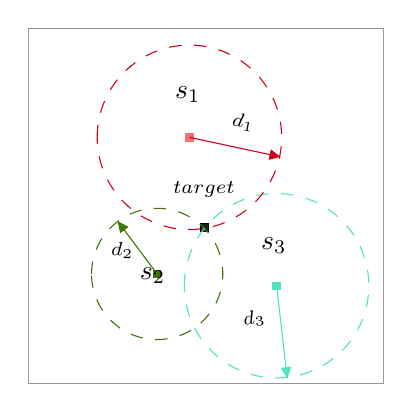
\begin{tikzpicture}[x=0.75pt,y=0.75pt,yscale=-1,xscale=1]
%uncomment if require: \path (0,300); %set diagram left start at 0, and has height of 300

%Shape: Square [id:dp3139397432452311] 
\draw  [color={rgb, 255:red, 154; green, 150; blue, 150 }  ,draw opacity=1 ] (75,51) -- (246,51) -- (246,222) -- (75,222) -- cycle ;
%Shape: Square [id:dp6615824497311407] 
\draw  [fill={rgb, 255:red, 33; green, 33; blue, 33 }  ,fill opacity=1 ] (157.96,145) -- (162,145) -- (162,149.04) -- (157.96,149.04) -- cycle ;
%Shape: Square [id:dp7238674463227524] 
\draw  [draw opacity=0][fill={rgb, 255:red, 80; green, 227; blue, 194 }  ,fill opacity=1 ] (192.64,173.04) -- (196.68,173.04) -- (196.68,177.08) -- (192.64,177.08) -- cycle ;
%Shape: Square [id:dp08550191202342461] 
\draw  [draw opacity=0][fill={rgb, 255:red, 248; green, 112; blue, 112 }  ,fill opacity=1 ] (150.64,101.54) -- (154.68,101.54) -- (154.68,105.58) -- (150.64,105.58) -- cycle ;
%Shape: Square [id:dp7141151551550344] 
\draw  [draw opacity=0][fill={rgb, 255:red, 65; green, 117; blue, 5 }  ,fill opacity=1 ] (135.1,167.36) -- (139.14,167.36) -- (139.14,171.4) -- (135.1,171.4) -- cycle ;
%Shape: Circle [id:dp9475883625678077] 
\draw  [color={rgb, 255:red, 65; green, 117; blue, 5 }  ,draw opacity=1 ][dash pattern={on 4.5pt off 4.5pt}] (105.5,169.38) .. controls (105.5,151.92) and (119.66,137.76) .. (137.12,137.76) .. controls (154.58,137.76) and (168.74,151.92) .. (168.74,169.38) .. controls (168.74,186.84) and (154.58,201) .. (137.12,201) .. controls (119.66,201) and (105.5,186.84) .. (105.5,169.38) -- cycle ;
%Shape: Circle [id:dp7445719218104008] 
\draw  [color={rgb, 255:red, 80; green, 227; blue, 194 }  ,draw opacity=1 ][dash pattern={on 4.5pt off 4.5pt}] (150.22,175.06) .. controls (150.22,150.52) and (170.12,130.62) .. (194.66,130.62) .. controls (219.2,130.62) and (239.1,150.52) .. (239.1,175.06) .. controls (239.1,199.6) and (219.2,219.5) .. (194.66,219.5) .. controls (170.12,219.5) and (150.22,199.6) .. (150.22,175.06) -- cycle ;
%Shape: Circle [id:dp34573460581909865] 
\draw  [color={rgb, 255:red, 208; green, 2; blue, 27 }  ,draw opacity=1 ][dash pattern={on 4.5pt off 4.5pt}] (108.22,103.56) .. controls (108.22,79.02) and (128.12,59.12) .. (152.66,59.12) .. controls (177.2,59.12) and (197.1,79.02) .. (197.1,103.56) .. controls (197.1,128.1) and (177.2,148) .. (152.66,148) .. controls (128.12,148) and (108.22,128.1) .. (108.22,103.56) -- cycle ;
%Straight Lines [id:da1278538436839034] 
\draw [color={rgb, 255:red, 208; green, 2; blue, 27 }  ,draw opacity=1 ]   (152.66,103.56) -- (193.65,112.37) ;
\draw [shift={(196.58,113)}, rotate = 192.13] [fill={rgb, 255:red, 208; green, 2; blue, 27 }  ,fill opacity=1 ][line width=0.08]  [draw opacity=0] (5.36,-2.57) -- (0,0) -- (5.36,2.57) -- cycle    ;
%Straight Lines [id:da7908947105774531] 
\draw [color={rgb, 255:red, 80; green, 227; blue, 194 }  ,draw opacity=1 ]   (194.66,175.06) -- (199.46,216.71) ;
\draw [shift={(199.81,219.69)}, rotate = 263.42] [fill={rgb, 255:red, 80; green, 227; blue, 194 }  ,fill opacity=1 ][line width=0.08]  [draw opacity=0] (5.36,-2.57) -- (0,0) -- (5.36,2.57) -- cycle    ;
%Straight Lines [id:da5760661930443354] 
\draw [color={rgb, 255:red, 65; green, 117; blue, 5 }  ,draw opacity=1 ]   (137.12,169.38) -- (119.9,146.38) ;
\draw [shift={(118.1,143.98)}, rotate = 53.17] [fill={rgb, 255:red, 65; green, 117; blue, 5 }  ,fill opacity=1 ][line width=0.08]  [draw opacity=0] (5.36,-2.57) -- (0,0) -- (5.36,2.57) -- cycle    ;


% Text Node
\draw (113.8,152.74) node [anchor=north west][inner sep=0.75pt]  [font=\scriptsize,rotate=-1.68] [align=left] {$\displaystyle d_{2}$};
% Text Node
\draw (176.58,186.84) node [anchor=north west][inner sep=0.75pt]  [font=\scriptsize,rotate=-351.95] [align=left] {$\displaystyle d_{3}$};
% Text Node
\draw (173.06,89.98) node [anchor=north west][inner sep=0.75pt]  [font=\scriptsize,rotate=-10.92] [align=left] {$\displaystyle d_{1}$};
% Text Node
\draw (143.5,123.5) node [anchor=north west][inner sep=0.75pt]  [font=\scriptsize] [align=left] {$\displaystyle target$};
% Text Node
\draw (186,150.5) node [anchor=north west][inner sep=0.75pt]   [align=left] {$\displaystyle s_{3}$};
% Text Node
\draw (127.5,165) node [anchor=north west][inner sep=0.75pt]   [align=left] {$\displaystyle s_{2}$};
% Text Node
\draw (144.5,78) node [anchor=north west][inner sep=0.75pt]   [align=left] {$\displaystyle s_{1}$};


\end{tikzpicture}}
  \caption{Ideal case of ToA solution}
  \label{fig:sub1}
\end{subfigure}%
\begin{subfigure}{0.5\textwidth}
 \centering
   \scalebox{.9}{


\tikzset{every picture/.style={line width=0.75pt}} %set default line width to 0.75pt        

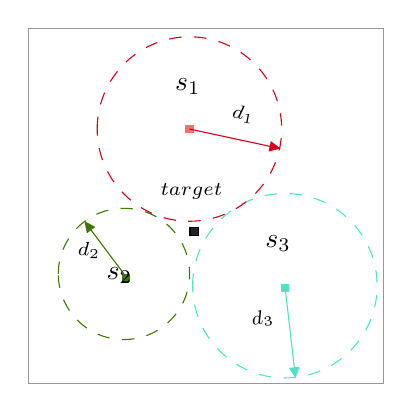
\begin{tikzpicture}[x=0.75pt,y=0.75pt,yscale=-1,xscale=1]
%uncomment if require: \path (0,300); %set diagram left start at 0, and has height of 300

%Shape: Square [id:dp9485406093696858] 
\draw  [color={rgb, 255:red, 154; green, 150; blue, 150 }  ,draw opacity=1 ] (314.5,50) -- (485.5,50) -- (485.5,221) -- (314.5,221) -- cycle ;
%Shape: Square [id:dp24929171411689466] 
\draw  [fill={rgb, 255:red, 33; green, 33; blue, 33 }  ,fill opacity=1 ] (392.46,146) -- (396.5,146) -- (396.5,150.04) -- (392.46,150.04) -- cycle ;
%Shape: Square [id:dp1889342057393233] 
\draw  [draw opacity=0][fill={rgb, 255:red, 80; green, 227; blue, 194 }  ,fill opacity=1 ] (436.14,173.04) -- (440.18,173.04) -- (440.18,177.08) -- (436.14,177.08) -- cycle ;
%Shape: Square [id:dp8116603792961381] 
\draw  [draw opacity=0][fill={rgb, 255:red, 248; green, 112; blue, 112 }  ,fill opacity=1 ] (390.14,96.54) -- (394.18,96.54) -- (394.18,100.58) -- (390.14,100.58) -- cycle ;
%Shape: Square [id:dp9501811324924574] 
\draw  [draw opacity=0][fill={rgb, 255:red, 65; green, 117; blue, 5 }  ,fill opacity=1 ] (359.6,168.36) -- (363.64,168.36) -- (363.64,172.4) -- (359.6,172.4) -- cycle ;
%Shape: Circle [id:dp3035334876106732] 
\draw  [color={rgb, 255:red, 65; green, 117; blue, 5 }  ,draw opacity=1 ][dash pattern={on 4.5pt off 4.5pt}] (329,168.38) .. controls (329,150.92) and (343.16,136.76) .. (360.62,136.76) .. controls (378.08,136.76) and (392.24,150.92) .. (392.24,168.38) .. controls (392.24,185.84) and (378.08,200) .. (360.62,200) .. controls (343.16,200) and (329,185.84) .. (329,168.38) -- cycle ;
%Shape: Circle [id:dp45289907486973524] 
\draw  [color={rgb, 255:red, 80; green, 227; blue, 194 }  ,draw opacity=1 ][dash pattern={on 4.5pt off 4.5pt}] (393.72,174.06) .. controls (393.72,149.52) and (413.62,129.62) .. (438.16,129.62) .. controls (462.7,129.62) and (482.6,149.52) .. (482.6,174.06) .. controls (482.6,198.6) and (462.7,218.5) .. (438.16,218.5) .. controls (413.62,218.5) and (393.72,198.6) .. (393.72,174.06) -- cycle ;
%Shape: Circle [id:dp28040021357673117] 
\draw  [color={rgb, 255:red, 208; green, 2; blue, 27 }  ,draw opacity=1 ][dash pattern={on 4.5pt off 4.5pt}] (347.72,98.56) .. controls (347.72,74.02) and (367.62,54.12) .. (392.16,54.12) .. controls (416.7,54.12) and (436.6,74.02) .. (436.6,98.56) .. controls (436.6,123.1) and (416.7,143) .. (392.16,143) .. controls (367.62,143) and (347.72,123.1) .. (347.72,98.56) -- cycle ;
%Straight Lines [id:da7421212837849427] 
\draw [color={rgb, 255:red, 208; green, 2; blue, 27 }  ,draw opacity=1 ]   (392.16,98.56) -- (433.15,107.37) ;
\draw [shift={(436.08,108)}, rotate = 192.13] [fill={rgb, 255:red, 208; green, 2; blue, 27 }  ,fill opacity=1 ][line width=0.08]  [draw opacity=0] (5.36,-2.57) -- (0,0) -- (5.36,2.57) -- cycle    ;
%Straight Lines [id:da6428590261529223] 
\draw [color={rgb, 255:red, 80; green, 227; blue, 194 }  ,draw opacity=1 ]   (438.16,174.06) -- (442.96,215.71) ;
\draw [shift={(443.31,218.69)}, rotate = 263.42] [fill={rgb, 255:red, 80; green, 227; blue, 194 }  ,fill opacity=1 ][line width=0.08]  [draw opacity=0] (5.36,-2.57) -- (0,0) -- (5.36,2.57) -- cycle    ;
%Straight Lines [id:da39676588633255805] 
\draw [color={rgb, 255:red, 65; green, 117; blue, 5 }  ,draw opacity=1 ]   (360.62,168.38) -- (343.4,145.38) ;
\draw [shift={(341.6,142.98)}, rotate = 53.17] [fill={rgb, 255:red, 65; green, 117; blue, 5 }  ,fill opacity=1 ][line width=0.08]  [draw opacity=0] (5.36,-2.57) -- (0,0) -- (5.36,2.57) -- cycle    ;


% Text Node
\draw (337.3,151.74) node [anchor=north west][inner sep=0.75pt]  [font=\scriptsize,rotate=-1.68] [align=left] {$\displaystyle d_{2}$};
% Text Node
\draw (420.08,185.84) node [anchor=north west][inner sep=0.75pt]  [font=\scriptsize,rotate=-351.95] [align=left] {$\displaystyle d_{3}$};
% Text Node
\draw (412.56,84.98) node [anchor=north west][inner sep=0.75pt]  [font=\scriptsize,rotate=-10.92] [align=left] {$\displaystyle d_{1}$};
% Text Node
\draw (377,123.5) node [anchor=north west][inner sep=0.75pt]  [font=\scriptsize] [align=left] {$\displaystyle target$};
% Text Node
\draw (427.5,148.5) node [anchor=north west][inner sep=0.75pt]   [align=left] {$\displaystyle s_{3}$};
% Text Node
\draw (351,164) node [anchor=north west][inner sep=0.75pt]   [align=left] {$\displaystyle s_{2}$};
% Text Node
\draw (384,73) node [anchor=north west][inner sep=0.75pt]   [align=left] {$\displaystyle s_{1}$};


\end{tikzpicture}}
  \caption{non-ideal case of ToA}
  \label{fig:sub2}
\end{subfigure}
\caption{ToA solution visuliazation}
\label{fig:test}
\end{figure}


\subsection{Time Difference of Arrival
(TDoA)}

TDoA is the second most popular technique, it is somehow more versatile
than ToA as this method does not require the time that the signal was
sent from the AE source, only the arrival time and signal speed are
needed to localize the source. Once two sensors at least (in 1-D)
receives the signal, we can compute the difference in arrival time and
hence, the difference of distance between the sensors and target. This
can follow the upcoming equation:\\
{\[\Delta d_{i,j} = v\ .\ \Delta t_{i,j}\]}In the 2-D case, however, the
equation can be written as follows:\\
{\[\Delta d_{i,j} = \sqrt{(x_{i}\  - x_{s})^{2} + (y_{i}\  - y_{s})^{2}} - \sqrt{(x_{j}\  - x_{s})^{2} + (y_{j}\  - y_{s})^{2}}\]}{\[where:\quad 1 \leq i,j \leq n\quad,\ i \neq j\]}And
{\(n\)} is the number of sensors in the sensor array. DToA is quite hard
to solve as there is not an obvious closed form solution . The solution
can rely on an optimization algorithm, which , in turn, tries to
minimize the difference between the calculated time difference and the
observed one:\\
{\[f(x,y) = \sum\limits_{i = 1}^{n}(\Delta t_{i,obs} - \Delta t_{i,clc})^{2}\]}Where:\\
{\[\Delta t_{i,obs} = t_{i} - t_{1}\]}{\[\Delta t_{i,clc} = \left\lbrack \sqrt{(x_{i}\  - x_{s})^{2} + (y_{i}\  - y_{s})^{2}} - \sqrt{(x_{1}\  - x_{s})^{2} + (y_{1}\  - y_{s})^{2}}\  \right\rbrack/v\]}So
our main goal is :\\
{\[\min\limits_{x,y\  \in \ R^{2}}\{ f(x,y)\}\]} And this will be
discussed in the optimization part. Now, the important question is how
to compute {\(t_{i}\)} for a given waveform. Some methods are going to
be introduced in the next section.


\section{Computation of arrival time}


\subsection{Threshold Crossing}

Generally, there are two main techniques used to compute the arrival
time of the signal to a given sensor. The first one is threshold
crossing, where a fraction {\(\alpha\)} of the maximum amplitude is set
as a minimum threshold, and then we have to iterate over the data points
until we have the first crossing. It is somehow a simple approach, and
not computationally expensive. In fact its complexity is fraction of
{\(n\)} or formally {\(\theta(n)\)} , where {\(n\)} is the number of
samples in the waveform.

\begin{figure}[htbp]
  \centering
  \scalebox{.5}{%% Creator: Matplotlib, PGF backend
%%
%% To include the figure in your LaTeX document, write
%%   \input{<filename>.pgf}
%%
%% Make sure the required packages are loaded in your preamble
%%   \usepackage{pgf}
%%
%% Also ensure that all the required font packages are loaded; for instance,
%% the lmodern package is sometimes necessary when using math font.
%%   \usepackage{lmodern}
%%
%% Figures using additional raster images can only be included by \input if
%% they are in the same directory as the main LaTeX file. For loading figures
%% from other directories you can use the `import` package
%%   \usepackage{import}
%%
%% and then include the figures with
%%   \import{<path to file>}{<filename>.pgf}
%%
%% Matplotlib used the following preamble
%%
\begingroup%
\makeatletter%
\begin{pgfpicture}%
\pgfpathrectangle{\pgfpointorigin}{\pgfqpoint{8.941365in}{6.323786in}}%
\pgfusepath{use as bounding box, clip}%
\begin{pgfscope}%
\pgfsetbuttcap%
\pgfsetmiterjoin%
\definecolor{currentfill}{rgb}{1.000000,1.000000,1.000000}%
\pgfsetfillcolor{currentfill}%
\pgfsetlinewidth{0.000000pt}%
\definecolor{currentstroke}{rgb}{1.000000,1.000000,1.000000}%
\pgfsetstrokecolor{currentstroke}%
\pgfsetdash{}{0pt}%
\pgfpathmoveto{\pgfqpoint{0.000000in}{0.000000in}}%
\pgfpathlineto{\pgfqpoint{8.941365in}{0.000000in}}%
\pgfpathlineto{\pgfqpoint{8.941365in}{6.323786in}}%
\pgfpathlineto{\pgfqpoint{0.000000in}{6.323786in}}%
\pgfpathlineto{\pgfqpoint{0.000000in}{0.000000in}}%
\pgfpathclose%
\pgfusepath{fill}%
\end{pgfscope}%
\begin{pgfscope}%
\pgfsetbuttcap%
\pgfsetmiterjoin%
\definecolor{currentfill}{rgb}{1.000000,1.000000,1.000000}%
\pgfsetfillcolor{currentfill}%
\pgfsetlinewidth{0.000000pt}%
\definecolor{currentstroke}{rgb}{0.000000,0.000000,0.000000}%
\pgfsetstrokecolor{currentstroke}%
\pgfsetstrokeopacity{0.000000}%
\pgfsetdash{}{0pt}%
\pgfpathmoveto{\pgfqpoint{0.781365in}{0.718286in}}%
\pgfpathlineto{\pgfqpoint{8.841365in}{0.718286in}}%
\pgfpathlineto{\pgfqpoint{8.841365in}{6.223786in}}%
\pgfpathlineto{\pgfqpoint{0.781365in}{6.223786in}}%
\pgfpathlineto{\pgfqpoint{0.781365in}{0.718286in}}%
\pgfpathclose%
\pgfusepath{fill}%
\end{pgfscope}%
\begin{pgfscope}%
\pgfpathrectangle{\pgfqpoint{0.781365in}{0.718286in}}{\pgfqpoint{8.060000in}{5.505500in}}%
\pgfusepath{clip}%
\pgfsetrectcap%
\pgfsetroundjoin%
\pgfsetlinewidth{1.304875pt}%
\definecolor{currentstroke}{rgb}{0.690196,0.690196,0.690196}%
\pgfsetstrokecolor{currentstroke}%
\pgfsetdash{}{0pt}%
\pgfpathmoveto{\pgfqpoint{2.167393in}{0.718286in}}%
\pgfpathlineto{\pgfqpoint{2.167393in}{6.223786in}}%
\pgfusepath{stroke}%
\end{pgfscope}%
\begin{pgfscope}%
\pgfsetbuttcap%
\pgfsetroundjoin%
\definecolor{currentfill}{rgb}{0.000000,0.000000,0.000000}%
\pgfsetfillcolor{currentfill}%
\pgfsetlinewidth{1.304875pt}%
\definecolor{currentstroke}{rgb}{0.000000,0.000000,0.000000}%
\pgfsetstrokecolor{currentstroke}%
\pgfsetdash{}{0pt}%
\pgfsys@defobject{currentmarker}{\pgfqpoint{0.000000in}{-0.048611in}}{\pgfqpoint{0.000000in}{0.000000in}}{%
\pgfpathmoveto{\pgfqpoint{0.000000in}{0.000000in}}%
\pgfpathlineto{\pgfqpoint{0.000000in}{-0.048611in}}%
\pgfusepath{stroke,fill}%
}%
\begin{pgfscope}%
\pgfsys@transformshift{2.167393in}{0.718286in}%
\pgfsys@useobject{currentmarker}{}%
\end{pgfscope}%
\end{pgfscope}%
\begin{pgfscope}%
\definecolor{textcolor}{rgb}{0.000000,0.000000,0.000000}%
\pgfsetstrokecolor{textcolor}%
\pgfsetfillcolor{textcolor}%
\pgftext[x=2.167393in,y=0.543286in,,top]{\color{textcolor}\rmfamily\fontsize{13.000000}{15.600000}\selectfont \(\displaystyle {8.41200}\)}%
\end{pgfscope}%
\begin{pgfscope}%
\pgfpathrectangle{\pgfqpoint{0.781365in}{0.718286in}}{\pgfqpoint{8.060000in}{5.505500in}}%
\pgfusepath{clip}%
\pgfsetrectcap%
\pgfsetroundjoin%
\pgfsetlinewidth{1.304875pt}%
\definecolor{currentstroke}{rgb}{0.690196,0.690196,0.690196}%
\pgfsetstrokecolor{currentstroke}%
\pgfsetdash{}{0pt}%
\pgfpathmoveto{\pgfqpoint{3.956278in}{0.718286in}}%
\pgfpathlineto{\pgfqpoint{3.956278in}{6.223786in}}%
\pgfusepath{stroke}%
\end{pgfscope}%
\begin{pgfscope}%
\pgfsetbuttcap%
\pgfsetroundjoin%
\definecolor{currentfill}{rgb}{0.000000,0.000000,0.000000}%
\pgfsetfillcolor{currentfill}%
\pgfsetlinewidth{1.304875pt}%
\definecolor{currentstroke}{rgb}{0.000000,0.000000,0.000000}%
\pgfsetstrokecolor{currentstroke}%
\pgfsetdash{}{0pt}%
\pgfsys@defobject{currentmarker}{\pgfqpoint{0.000000in}{-0.048611in}}{\pgfqpoint{0.000000in}{0.000000in}}{%
\pgfpathmoveto{\pgfqpoint{0.000000in}{0.000000in}}%
\pgfpathlineto{\pgfqpoint{0.000000in}{-0.048611in}}%
\pgfusepath{stroke,fill}%
}%
\begin{pgfscope}%
\pgfsys@transformshift{3.956278in}{0.718286in}%
\pgfsys@useobject{currentmarker}{}%
\end{pgfscope}%
\end{pgfscope}%
\begin{pgfscope}%
\definecolor{textcolor}{rgb}{0.000000,0.000000,0.000000}%
\pgfsetstrokecolor{textcolor}%
\pgfsetfillcolor{textcolor}%
\pgftext[x=3.956278in,y=0.543286in,,top]{\color{textcolor}\rmfamily\fontsize{13.000000}{15.600000}\selectfont \(\displaystyle {8.41205}\)}%
\end{pgfscope}%
\begin{pgfscope}%
\pgfpathrectangle{\pgfqpoint{0.781365in}{0.718286in}}{\pgfqpoint{8.060000in}{5.505500in}}%
\pgfusepath{clip}%
\pgfsetrectcap%
\pgfsetroundjoin%
\pgfsetlinewidth{1.304875pt}%
\definecolor{currentstroke}{rgb}{0.690196,0.690196,0.690196}%
\pgfsetstrokecolor{currentstroke}%
\pgfsetdash{}{0pt}%
\pgfpathmoveto{\pgfqpoint{5.745163in}{0.718286in}}%
\pgfpathlineto{\pgfqpoint{5.745163in}{6.223786in}}%
\pgfusepath{stroke}%
\end{pgfscope}%
\begin{pgfscope}%
\pgfsetbuttcap%
\pgfsetroundjoin%
\definecolor{currentfill}{rgb}{0.000000,0.000000,0.000000}%
\pgfsetfillcolor{currentfill}%
\pgfsetlinewidth{1.304875pt}%
\definecolor{currentstroke}{rgb}{0.000000,0.000000,0.000000}%
\pgfsetstrokecolor{currentstroke}%
\pgfsetdash{}{0pt}%
\pgfsys@defobject{currentmarker}{\pgfqpoint{0.000000in}{-0.048611in}}{\pgfqpoint{0.000000in}{0.000000in}}{%
\pgfpathmoveto{\pgfqpoint{0.000000in}{0.000000in}}%
\pgfpathlineto{\pgfqpoint{0.000000in}{-0.048611in}}%
\pgfusepath{stroke,fill}%
}%
\begin{pgfscope}%
\pgfsys@transformshift{5.745163in}{0.718286in}%
\pgfsys@useobject{currentmarker}{}%
\end{pgfscope}%
\end{pgfscope}%
\begin{pgfscope}%
\definecolor{textcolor}{rgb}{0.000000,0.000000,0.000000}%
\pgfsetstrokecolor{textcolor}%
\pgfsetfillcolor{textcolor}%
\pgftext[x=5.745163in,y=0.543286in,,top]{\color{textcolor}\rmfamily\fontsize{13.000000}{15.600000}\selectfont \(\displaystyle {8.41210}\)}%
\end{pgfscope}%
\begin{pgfscope}%
\pgfpathrectangle{\pgfqpoint{0.781365in}{0.718286in}}{\pgfqpoint{8.060000in}{5.505500in}}%
\pgfusepath{clip}%
\pgfsetrectcap%
\pgfsetroundjoin%
\pgfsetlinewidth{1.304875pt}%
\definecolor{currentstroke}{rgb}{0.690196,0.690196,0.690196}%
\pgfsetstrokecolor{currentstroke}%
\pgfsetdash{}{0pt}%
\pgfpathmoveto{\pgfqpoint{7.534048in}{0.718286in}}%
\pgfpathlineto{\pgfqpoint{7.534048in}{6.223786in}}%
\pgfusepath{stroke}%
\end{pgfscope}%
\begin{pgfscope}%
\pgfsetbuttcap%
\pgfsetroundjoin%
\definecolor{currentfill}{rgb}{0.000000,0.000000,0.000000}%
\pgfsetfillcolor{currentfill}%
\pgfsetlinewidth{1.304875pt}%
\definecolor{currentstroke}{rgb}{0.000000,0.000000,0.000000}%
\pgfsetstrokecolor{currentstroke}%
\pgfsetdash{}{0pt}%
\pgfsys@defobject{currentmarker}{\pgfqpoint{0.000000in}{-0.048611in}}{\pgfqpoint{0.000000in}{0.000000in}}{%
\pgfpathmoveto{\pgfqpoint{0.000000in}{0.000000in}}%
\pgfpathlineto{\pgfqpoint{0.000000in}{-0.048611in}}%
\pgfusepath{stroke,fill}%
}%
\begin{pgfscope}%
\pgfsys@transformshift{7.534048in}{0.718286in}%
\pgfsys@useobject{currentmarker}{}%
\end{pgfscope}%
\end{pgfscope}%
\begin{pgfscope}%
\definecolor{textcolor}{rgb}{0.000000,0.000000,0.000000}%
\pgfsetstrokecolor{textcolor}%
\pgfsetfillcolor{textcolor}%
\pgftext[x=7.534048in,y=0.543286in,,top]{\color{textcolor}\rmfamily\fontsize{13.000000}{15.600000}\selectfont \(\displaystyle {8.41215}\)}%
\end{pgfscope}%
\begin{pgfscope}%
\definecolor{textcolor}{rgb}{0.000000,0.000000,0.000000}%
\pgfsetstrokecolor{textcolor}%
\pgfsetfillcolor{textcolor}%
\pgftext[x=4.811365in,y=0.339583in,,top]{\color{textcolor}\rmfamily\fontsize{17.000000}{20.400000}\selectfont time \(\displaystyle [s]\)}%
\end{pgfscope}%
\begin{pgfscope}%
\pgfpathrectangle{\pgfqpoint{0.781365in}{0.718286in}}{\pgfqpoint{8.060000in}{5.505500in}}%
\pgfusepath{clip}%
\pgfsetrectcap%
\pgfsetroundjoin%
\pgfsetlinewidth{1.304875pt}%
\definecolor{currentstroke}{rgb}{0.690196,0.690196,0.690196}%
\pgfsetstrokecolor{currentstroke}%
\pgfsetdash{}{0pt}%
\pgfpathmoveto{\pgfqpoint{0.781365in}{1.518317in}}%
\pgfpathlineto{\pgfqpoint{8.841365in}{1.518317in}}%
\pgfusepath{stroke}%
\end{pgfscope}%
\begin{pgfscope}%
\pgfsetbuttcap%
\pgfsetroundjoin%
\definecolor{currentfill}{rgb}{0.000000,0.000000,0.000000}%
\pgfsetfillcolor{currentfill}%
\pgfsetlinewidth{1.304875pt}%
\definecolor{currentstroke}{rgb}{0.000000,0.000000,0.000000}%
\pgfsetstrokecolor{currentstroke}%
\pgfsetdash{}{0pt}%
\pgfsys@defobject{currentmarker}{\pgfqpoint{-0.048611in}{0.000000in}}{\pgfqpoint{-0.000000in}{0.000000in}}{%
\pgfpathmoveto{\pgfqpoint{-0.000000in}{0.000000in}}%
\pgfpathlineto{\pgfqpoint{-0.048611in}{0.000000in}}%
\pgfusepath{stroke,fill}%
}%
\begin{pgfscope}%
\pgfsys@transformshift{0.781365in}{1.518317in}%
\pgfsys@useobject{currentmarker}{}%
\end{pgfscope}%
\end{pgfscope}%
\begin{pgfscope}%
\definecolor{textcolor}{rgb}{0.000000,0.000000,0.000000}%
\pgfsetstrokecolor{textcolor}%
\pgfsetfillcolor{textcolor}%
\pgftext[x=0.395138in, y=1.460447in, left, base]{\color{textcolor}\rmfamily\fontsize{13.000000}{15.600000}\selectfont \(\displaystyle {\ensuremath{-}2}\)}%
\end{pgfscope}%
\begin{pgfscope}%
\pgfpathrectangle{\pgfqpoint{0.781365in}{0.718286in}}{\pgfqpoint{8.060000in}{5.505500in}}%
\pgfusepath{clip}%
\pgfsetrectcap%
\pgfsetroundjoin%
\pgfsetlinewidth{1.304875pt}%
\definecolor{currentstroke}{rgb}{0.690196,0.690196,0.690196}%
\pgfsetstrokecolor{currentstroke}%
\pgfsetdash{}{0pt}%
\pgfpathmoveto{\pgfqpoint{0.781365in}{2.576543in}}%
\pgfpathlineto{\pgfqpoint{8.841365in}{2.576543in}}%
\pgfusepath{stroke}%
\end{pgfscope}%
\begin{pgfscope}%
\pgfsetbuttcap%
\pgfsetroundjoin%
\definecolor{currentfill}{rgb}{0.000000,0.000000,0.000000}%
\pgfsetfillcolor{currentfill}%
\pgfsetlinewidth{1.304875pt}%
\definecolor{currentstroke}{rgb}{0.000000,0.000000,0.000000}%
\pgfsetstrokecolor{currentstroke}%
\pgfsetdash{}{0pt}%
\pgfsys@defobject{currentmarker}{\pgfqpoint{-0.048611in}{0.000000in}}{\pgfqpoint{-0.000000in}{0.000000in}}{%
\pgfpathmoveto{\pgfqpoint{-0.000000in}{0.000000in}}%
\pgfpathlineto{\pgfqpoint{-0.048611in}{0.000000in}}%
\pgfusepath{stroke,fill}%
}%
\begin{pgfscope}%
\pgfsys@transformshift{0.781365in}{2.576543in}%
\pgfsys@useobject{currentmarker}{}%
\end{pgfscope}%
\end{pgfscope}%
\begin{pgfscope}%
\definecolor{textcolor}{rgb}{0.000000,0.000000,0.000000}%
\pgfsetstrokecolor{textcolor}%
\pgfsetfillcolor{textcolor}%
\pgftext[x=0.395138in, y=2.518673in, left, base]{\color{textcolor}\rmfamily\fontsize{13.000000}{15.600000}\selectfont \(\displaystyle {\ensuremath{-}1}\)}%
\end{pgfscope}%
\begin{pgfscope}%
\pgfpathrectangle{\pgfqpoint{0.781365in}{0.718286in}}{\pgfqpoint{8.060000in}{5.505500in}}%
\pgfusepath{clip}%
\pgfsetrectcap%
\pgfsetroundjoin%
\pgfsetlinewidth{1.304875pt}%
\definecolor{currentstroke}{rgb}{0.690196,0.690196,0.690196}%
\pgfsetstrokecolor{currentstroke}%
\pgfsetdash{}{0pt}%
\pgfpathmoveto{\pgfqpoint{0.781365in}{3.634769in}}%
\pgfpathlineto{\pgfqpoint{8.841365in}{3.634769in}}%
\pgfusepath{stroke}%
\end{pgfscope}%
\begin{pgfscope}%
\pgfsetbuttcap%
\pgfsetroundjoin%
\definecolor{currentfill}{rgb}{0.000000,0.000000,0.000000}%
\pgfsetfillcolor{currentfill}%
\pgfsetlinewidth{1.304875pt}%
\definecolor{currentstroke}{rgb}{0.000000,0.000000,0.000000}%
\pgfsetstrokecolor{currentstroke}%
\pgfsetdash{}{0pt}%
\pgfsys@defobject{currentmarker}{\pgfqpoint{-0.048611in}{0.000000in}}{\pgfqpoint{-0.000000in}{0.000000in}}{%
\pgfpathmoveto{\pgfqpoint{-0.000000in}{0.000000in}}%
\pgfpathlineto{\pgfqpoint{-0.048611in}{0.000000in}}%
\pgfusepath{stroke,fill}%
}%
\begin{pgfscope}%
\pgfsys@transformshift{0.781365in}{3.634769in}%
\pgfsys@useobject{currentmarker}{}%
\end{pgfscope}%
\end{pgfscope}%
\begin{pgfscope}%
\definecolor{textcolor}{rgb}{0.000000,0.000000,0.000000}%
\pgfsetstrokecolor{textcolor}%
\pgfsetfillcolor{textcolor}%
\pgftext[x=0.524768in, y=3.576899in, left, base]{\color{textcolor}\rmfamily\fontsize{13.000000}{15.600000}\selectfont \(\displaystyle {0}\)}%
\end{pgfscope}%
\begin{pgfscope}%
\pgfpathrectangle{\pgfqpoint{0.781365in}{0.718286in}}{\pgfqpoint{8.060000in}{5.505500in}}%
\pgfusepath{clip}%
\pgfsetrectcap%
\pgfsetroundjoin%
\pgfsetlinewidth{1.304875pt}%
\definecolor{currentstroke}{rgb}{0.690196,0.690196,0.690196}%
\pgfsetstrokecolor{currentstroke}%
\pgfsetdash{}{0pt}%
\pgfpathmoveto{\pgfqpoint{0.781365in}{4.692995in}}%
\pgfpathlineto{\pgfqpoint{8.841365in}{4.692995in}}%
\pgfusepath{stroke}%
\end{pgfscope}%
\begin{pgfscope}%
\pgfsetbuttcap%
\pgfsetroundjoin%
\definecolor{currentfill}{rgb}{0.000000,0.000000,0.000000}%
\pgfsetfillcolor{currentfill}%
\pgfsetlinewidth{1.304875pt}%
\definecolor{currentstroke}{rgb}{0.000000,0.000000,0.000000}%
\pgfsetstrokecolor{currentstroke}%
\pgfsetdash{}{0pt}%
\pgfsys@defobject{currentmarker}{\pgfqpoint{-0.048611in}{0.000000in}}{\pgfqpoint{-0.000000in}{0.000000in}}{%
\pgfpathmoveto{\pgfqpoint{-0.000000in}{0.000000in}}%
\pgfpathlineto{\pgfqpoint{-0.048611in}{0.000000in}}%
\pgfusepath{stroke,fill}%
}%
\begin{pgfscope}%
\pgfsys@transformshift{0.781365in}{4.692995in}%
\pgfsys@useobject{currentmarker}{}%
\end{pgfscope}%
\end{pgfscope}%
\begin{pgfscope}%
\definecolor{textcolor}{rgb}{0.000000,0.000000,0.000000}%
\pgfsetstrokecolor{textcolor}%
\pgfsetfillcolor{textcolor}%
\pgftext[x=0.524768in, y=4.635125in, left, base]{\color{textcolor}\rmfamily\fontsize{13.000000}{15.600000}\selectfont \(\displaystyle {1}\)}%
\end{pgfscope}%
\begin{pgfscope}%
\pgfpathrectangle{\pgfqpoint{0.781365in}{0.718286in}}{\pgfqpoint{8.060000in}{5.505500in}}%
\pgfusepath{clip}%
\pgfsetrectcap%
\pgfsetroundjoin%
\pgfsetlinewidth{1.304875pt}%
\definecolor{currentstroke}{rgb}{0.690196,0.690196,0.690196}%
\pgfsetstrokecolor{currentstroke}%
\pgfsetdash{}{0pt}%
\pgfpathmoveto{\pgfqpoint{0.781365in}{5.751221in}}%
\pgfpathlineto{\pgfqpoint{8.841365in}{5.751221in}}%
\pgfusepath{stroke}%
\end{pgfscope}%
\begin{pgfscope}%
\pgfsetbuttcap%
\pgfsetroundjoin%
\definecolor{currentfill}{rgb}{0.000000,0.000000,0.000000}%
\pgfsetfillcolor{currentfill}%
\pgfsetlinewidth{1.304875pt}%
\definecolor{currentstroke}{rgb}{0.000000,0.000000,0.000000}%
\pgfsetstrokecolor{currentstroke}%
\pgfsetdash{}{0pt}%
\pgfsys@defobject{currentmarker}{\pgfqpoint{-0.048611in}{0.000000in}}{\pgfqpoint{-0.000000in}{0.000000in}}{%
\pgfpathmoveto{\pgfqpoint{-0.000000in}{0.000000in}}%
\pgfpathlineto{\pgfqpoint{-0.048611in}{0.000000in}}%
\pgfusepath{stroke,fill}%
}%
\begin{pgfscope}%
\pgfsys@transformshift{0.781365in}{5.751221in}%
\pgfsys@useobject{currentmarker}{}%
\end{pgfscope}%
\end{pgfscope}%
\begin{pgfscope}%
\definecolor{textcolor}{rgb}{0.000000,0.000000,0.000000}%
\pgfsetstrokecolor{textcolor}%
\pgfsetfillcolor{textcolor}%
\pgftext[x=0.524768in, y=5.693350in, left, base]{\color{textcolor}\rmfamily\fontsize{13.000000}{15.600000}\selectfont \(\displaystyle {2}\)}%
\end{pgfscope}%
\begin{pgfscope}%
\definecolor{textcolor}{rgb}{0.000000,0.000000,0.000000}%
\pgfsetstrokecolor{textcolor}%
\pgfsetfillcolor{textcolor}%
\pgftext[x=0.339583in,y=3.471036in,,bottom,rotate=90.000000]{\color{textcolor}\rmfamily\fontsize{17.000000}{20.400000}\selectfont Amplitude[V]}%
\end{pgfscope}%
\begin{pgfscope}%
\pgfpathrectangle{\pgfqpoint{0.781365in}{0.718286in}}{\pgfqpoint{8.060000in}{5.505500in}}%
\pgfusepath{clip}%
\pgfsetrectcap%
\pgfsetroundjoin%
\pgfsetlinewidth{1.003750pt}%
\definecolor{currentstroke}{rgb}{0.000000,0.000000,1.000000}%
\pgfsetstrokecolor{currentstroke}%
\pgfsetdash{}{0pt}%
\pgfpathmoveto{\pgfqpoint{1.147728in}{3.634123in}}%
\pgfpathlineto{\pgfqpoint{1.455717in}{3.633154in}}%
\pgfpathlineto{\pgfqpoint{1.477205in}{3.632831in}}%
\pgfpathlineto{\pgfqpoint{1.520180in}{3.633800in}}%
\pgfpathlineto{\pgfqpoint{1.613293in}{3.634769in}}%
\pgfpathlineto{\pgfqpoint{1.634781in}{3.634769in}}%
\pgfpathlineto{\pgfqpoint{1.756544in}{3.635738in}}%
\pgfpathlineto{\pgfqpoint{1.778032in}{3.637030in}}%
\pgfpathlineto{\pgfqpoint{1.792357in}{3.636707in}}%
\pgfpathlineto{\pgfqpoint{1.806682in}{3.632185in}}%
\pgfpathlineto{\pgfqpoint{1.821007in}{3.625081in}}%
\pgfpathlineto{\pgfqpoint{1.835332in}{3.617007in}}%
\pgfpathlineto{\pgfqpoint{1.842494in}{3.614101in}}%
\pgfpathlineto{\pgfqpoint{1.849657in}{3.613132in}}%
\pgfpathlineto{\pgfqpoint{1.856819in}{3.613778in}}%
\pgfpathlineto{\pgfqpoint{1.863982in}{3.617976in}}%
\pgfpathlineto{\pgfqpoint{1.871144in}{3.625727in}}%
\pgfpathlineto{\pgfqpoint{1.885470in}{3.648979in}}%
\pgfpathlineto{\pgfqpoint{1.899795in}{3.673845in}}%
\pgfpathlineto{\pgfqpoint{1.906957in}{3.682242in}}%
\pgfpathlineto{\pgfqpoint{1.914120in}{3.686440in}}%
\pgfpathlineto{\pgfqpoint{1.921282in}{3.684825in}}%
\pgfpathlineto{\pgfqpoint{1.928445in}{3.676106in}}%
\pgfpathlineto{\pgfqpoint{1.935607in}{3.662542in}}%
\pgfpathlineto{\pgfqpoint{1.964257in}{3.599245in}}%
\pgfpathlineto{\pgfqpoint{1.971420in}{3.590203in}}%
\pgfpathlineto{\pgfqpoint{1.978582in}{3.587296in}}%
\pgfpathlineto{\pgfqpoint{1.985745in}{3.590526in}}%
\pgfpathlineto{\pgfqpoint{1.992908in}{3.599891in}}%
\pgfpathlineto{\pgfqpoint{2.000070in}{3.614424in}}%
\pgfpathlineto{\pgfqpoint{2.021558in}{3.663511in}}%
\pgfpathlineto{\pgfqpoint{2.028720in}{3.673199in}}%
\pgfpathlineto{\pgfqpoint{2.035883in}{3.675783in}}%
\pgfpathlineto{\pgfqpoint{2.043045in}{3.670293in}}%
\pgfpathlineto{\pgfqpoint{2.050208in}{3.657375in}}%
\pgfpathlineto{\pgfqpoint{2.057370in}{3.637030in}}%
\pgfpathlineto{\pgfqpoint{2.071695in}{3.583421in}}%
\pgfpathlineto{\pgfqpoint{2.086021in}{3.531750in}}%
\pgfpathlineto{\pgfqpoint{2.093183in}{3.514956in}}%
\pgfpathlineto{\pgfqpoint{2.100346in}{3.509466in}}%
\pgfpathlineto{\pgfqpoint{2.107508in}{3.515925in}}%
\pgfpathlineto{\pgfqpoint{2.114671in}{3.534656in}}%
\pgfpathlineto{\pgfqpoint{2.121833in}{3.564367in}}%
\pgfpathlineto{\pgfqpoint{2.136158in}{3.646395in}}%
\pgfpathlineto{\pgfqpoint{2.150483in}{3.735528in}}%
\pgfpathlineto{\pgfqpoint{2.157646in}{3.770729in}}%
\pgfpathlineto{\pgfqpoint{2.164808in}{3.791074in}}%
\pgfpathlineto{\pgfqpoint{2.171971in}{3.792366in}}%
\pgfpathlineto{\pgfqpoint{2.179133in}{3.776219in}}%
\pgfpathlineto{\pgfqpoint{2.186296in}{3.745216in}}%
\pgfpathlineto{\pgfqpoint{2.193459in}{3.702587in}}%
\pgfpathlineto{\pgfqpoint{2.214946in}{3.550157in}}%
\pgfpathlineto{\pgfqpoint{2.222109in}{3.516248in}}%
\pgfpathlineto{\pgfqpoint{2.229271in}{3.499455in}}%
\pgfpathlineto{\pgfqpoint{2.236434in}{3.501070in}}%
\pgfpathlineto{\pgfqpoint{2.243596in}{3.520124in}}%
\pgfpathlineto{\pgfqpoint{2.250759in}{3.554679in}}%
\pgfpathlineto{\pgfqpoint{2.265084in}{3.655438in}}%
\pgfpathlineto{\pgfqpoint{2.279409in}{3.759749in}}%
\pgfpathlineto{\pgfqpoint{2.286571in}{3.794627in}}%
\pgfpathlineto{\pgfqpoint{2.293734in}{3.802377in}}%
\pgfpathlineto{\pgfqpoint{2.300897in}{3.783970in}}%
\pgfpathlineto{\pgfqpoint{2.308059in}{3.754259in}}%
\pgfpathlineto{\pgfqpoint{2.315222in}{3.719058in}}%
\pgfpathlineto{\pgfqpoint{2.322384in}{3.674168in}}%
\pgfpathlineto{\pgfqpoint{2.336709in}{3.558554in}}%
\pgfpathlineto{\pgfqpoint{2.351034in}{3.437127in}}%
\pgfpathlineto{\pgfqpoint{2.358197in}{3.386424in}}%
\pgfpathlineto{\pgfqpoint{2.365359in}{3.350900in}}%
\pgfpathlineto{\pgfqpoint{2.372522in}{3.337014in}}%
\pgfpathlineto{\pgfqpoint{2.379684in}{3.347348in}}%
\pgfpathlineto{\pgfqpoint{2.386847in}{3.381580in}}%
\pgfpathlineto{\pgfqpoint{2.394009in}{3.438741in}}%
\pgfpathlineto{\pgfqpoint{2.401172in}{3.517540in}}%
\pgfpathlineto{\pgfqpoint{2.415497in}{3.721964in}}%
\pgfpathlineto{\pgfqpoint{2.422660in}{3.826598in}}%
\pgfpathlineto{\pgfqpoint{2.429822in}{3.909918in}}%
\pgfpathlineto{\pgfqpoint{2.436985in}{3.967402in}}%
\pgfpathlineto{\pgfqpoint{2.444147in}{3.989685in}}%
\pgfpathlineto{\pgfqpoint{2.451310in}{3.951255in}}%
\pgfpathlineto{\pgfqpoint{2.465635in}{3.762978in}}%
\pgfpathlineto{\pgfqpoint{2.487122in}{3.468452in}}%
\pgfpathlineto{\pgfqpoint{2.494285in}{3.397082in}}%
\pgfpathlineto{\pgfqpoint{2.501448in}{3.355422in}}%
\pgfpathlineto{\pgfqpoint{2.508610in}{3.344765in}}%
\pgfpathlineto{\pgfqpoint{2.515773in}{3.363172in}}%
\pgfpathlineto{\pgfqpoint{2.522935in}{3.407416in}}%
\pgfpathlineto{\pgfqpoint{2.530098in}{3.472651in}}%
\pgfpathlineto{\pgfqpoint{2.551585in}{3.719704in}}%
\pgfpathlineto{\pgfqpoint{2.558748in}{3.783001in}}%
\pgfpathlineto{\pgfqpoint{2.565910in}{3.827567in}}%
\pgfpathlineto{\pgfqpoint{2.573073in}{3.838547in}}%
\pgfpathlineto{\pgfqpoint{2.580235in}{3.807867in}}%
\pgfpathlineto{\pgfqpoint{2.601723in}{3.666741in}}%
\pgfpathlineto{\pgfqpoint{2.616048in}{3.580191in}}%
\pgfpathlineto{\pgfqpoint{2.623211in}{3.552418in}}%
\pgfpathlineto{\pgfqpoint{2.630373in}{3.540146in}}%
\pgfpathlineto{\pgfqpoint{2.637536in}{3.542084in}}%
\pgfpathlineto{\pgfqpoint{2.644698in}{3.555970in}}%
\pgfpathlineto{\pgfqpoint{2.651861in}{3.579545in}}%
\pgfpathlineto{\pgfqpoint{2.687673in}{3.726485in}}%
\pgfpathlineto{\pgfqpoint{2.701998in}{3.765239in}}%
\pgfpathlineto{\pgfqpoint{2.716324in}{3.795596in}}%
\pgfpathlineto{\pgfqpoint{2.723486in}{3.806253in}}%
\pgfpathlineto{\pgfqpoint{2.730649in}{3.812389in}}%
\pgfpathlineto{\pgfqpoint{2.737811in}{3.812712in}}%
\pgfpathlineto{\pgfqpoint{2.744974in}{3.806899in}}%
\pgfpathlineto{\pgfqpoint{2.752136in}{3.794627in}}%
\pgfpathlineto{\pgfqpoint{2.759299in}{3.774604in}}%
\pgfpathlineto{\pgfqpoint{2.766461in}{3.746831in}}%
\pgfpathlineto{\pgfqpoint{2.780786in}{3.671585in}}%
\pgfpathlineto{\pgfqpoint{2.802274in}{3.543699in}}%
\pgfpathlineto{\pgfqpoint{2.809436in}{3.509143in}}%
\pgfpathlineto{\pgfqpoint{2.816599in}{3.482339in}}%
\pgfpathlineto{\pgfqpoint{2.823762in}{3.463285in}}%
\pgfpathlineto{\pgfqpoint{2.830924in}{3.451659in}}%
\pgfpathlineto{\pgfqpoint{2.838087in}{3.446169in}}%
\pgfpathlineto{\pgfqpoint{2.845249in}{3.445846in}}%
\pgfpathlineto{\pgfqpoint{2.852412in}{3.449722in}}%
\pgfpathlineto{\pgfqpoint{2.859574in}{3.458764in}}%
\pgfpathlineto{\pgfqpoint{2.866737in}{3.473297in}}%
\pgfpathlineto{\pgfqpoint{2.873899in}{3.494611in}}%
\pgfpathlineto{\pgfqpoint{2.881062in}{3.522061in}}%
\pgfpathlineto{\pgfqpoint{2.888224in}{3.556616in}}%
\pgfpathlineto{\pgfqpoint{2.902549in}{3.644457in}}%
\pgfpathlineto{\pgfqpoint{2.924037in}{3.793658in}}%
\pgfpathlineto{\pgfqpoint{2.931200in}{3.833057in}}%
\pgfpathlineto{\pgfqpoint{2.938362in}{3.855663in}}%
\pgfpathlineto{\pgfqpoint{2.945525in}{3.858247in}}%
\pgfpathlineto{\pgfqpoint{2.952687in}{3.844360in}}%
\pgfpathlineto{\pgfqpoint{2.959850in}{3.820139in}}%
\pgfpathlineto{\pgfqpoint{2.974175in}{3.752321in}}%
\pgfpathlineto{\pgfqpoint{2.981337in}{3.717443in}}%
\pgfpathlineto{\pgfqpoint{2.988500in}{3.690316in}}%
\pgfpathlineto{\pgfqpoint{2.995662in}{3.674491in}}%
\pgfpathlineto{\pgfqpoint{3.002825in}{3.670939in}}%
\pgfpathlineto{\pgfqpoint{3.009987in}{3.678690in}}%
\pgfpathlineto{\pgfqpoint{3.017150in}{3.694837in}}%
\pgfpathlineto{\pgfqpoint{3.031475in}{3.734559in}}%
\pgfpathlineto{\pgfqpoint{3.038638in}{3.744247in}}%
\pgfpathlineto{\pgfqpoint{3.045800in}{3.737466in}}%
\pgfpathlineto{\pgfqpoint{3.052963in}{3.709692in}}%
\pgfpathlineto{\pgfqpoint{3.060125in}{3.661251in}}%
\pgfpathlineto{\pgfqpoint{3.067288in}{3.594724in}}%
\pgfpathlineto{\pgfqpoint{3.081613in}{3.424855in}}%
\pgfpathlineto{\pgfqpoint{3.095938in}{3.254340in}}%
\pgfpathlineto{\pgfqpoint{3.103100in}{3.189428in}}%
\pgfpathlineto{\pgfqpoint{3.110263in}{3.145830in}}%
\pgfpathlineto{\pgfqpoint{3.117425in}{3.130975in}}%
\pgfpathlineto{\pgfqpoint{3.124588in}{3.143570in}}%
\pgfpathlineto{\pgfqpoint{3.131751in}{3.182646in}}%
\pgfpathlineto{\pgfqpoint{3.146076in}{3.302459in}}%
\pgfpathlineto{\pgfqpoint{3.174726in}{3.555970in}}%
\pgfpathlineto{\pgfqpoint{3.181888in}{3.583744in}}%
\pgfpathlineto{\pgfqpoint{3.189051in}{3.574701in}}%
\pgfpathlineto{\pgfqpoint{3.210538in}{3.466515in}}%
\pgfpathlineto{\pgfqpoint{3.232026in}{3.369308in}}%
\pgfpathlineto{\pgfqpoint{3.239189in}{3.345410in}}%
\pgfpathlineto{\pgfqpoint{3.246351in}{3.327971in}}%
\pgfpathlineto{\pgfqpoint{3.253514in}{3.316022in}}%
\pgfpathlineto{\pgfqpoint{3.267839in}{3.301167in}}%
\pgfpathlineto{\pgfqpoint{3.282164in}{3.296323in}}%
\pgfpathlineto{\pgfqpoint{3.289326in}{3.296000in}}%
\pgfpathlineto{\pgfqpoint{3.296489in}{3.297938in}}%
\pgfpathlineto{\pgfqpoint{3.303651in}{3.304073in}}%
\pgfpathlineto{\pgfqpoint{3.310814in}{3.319252in}}%
\pgfpathlineto{\pgfqpoint{3.317976in}{3.341212in}}%
\pgfpathlineto{\pgfqpoint{3.325139in}{3.372861in}}%
\pgfpathlineto{\pgfqpoint{3.332302in}{3.413552in}}%
\pgfpathlineto{\pgfqpoint{3.346627in}{3.517863in}}%
\pgfpathlineto{\pgfqpoint{3.368114in}{3.688055in}}%
\pgfpathlineto{\pgfqpoint{3.375277in}{3.727131in}}%
\pgfpathlineto{\pgfqpoint{3.382439in}{3.739403in}}%
\pgfpathlineto{\pgfqpoint{3.389602in}{3.718089in}}%
\pgfpathlineto{\pgfqpoint{3.396764in}{3.675783in}}%
\pgfpathlineto{\pgfqpoint{3.403927in}{3.623466in}}%
\pgfpathlineto{\pgfqpoint{3.418252in}{3.487829in}}%
\pgfpathlineto{\pgfqpoint{3.432577in}{3.355422in}}%
\pgfpathlineto{\pgfqpoint{3.439740in}{3.311178in}}%
\pgfpathlineto{\pgfqpoint{3.446902in}{3.288572in}}%
\pgfpathlineto{\pgfqpoint{3.454065in}{3.294385in}}%
\pgfpathlineto{\pgfqpoint{3.461227in}{3.325065in}}%
\pgfpathlineto{\pgfqpoint{3.468390in}{3.379643in}}%
\pgfpathlineto{\pgfqpoint{3.475552in}{3.458764in}}%
\pgfpathlineto{\pgfqpoint{3.482715in}{3.560492in}}%
\pgfpathlineto{\pgfqpoint{3.511365in}{4.035867in}}%
\pgfpathlineto{\pgfqpoint{3.518527in}{4.128229in}}%
\pgfpathlineto{\pgfqpoint{3.525690in}{4.205736in}}%
\pgfpathlineto{\pgfqpoint{3.532852in}{4.262574in}}%
\pgfpathlineto{\pgfqpoint{3.540015in}{4.301973in}}%
\pgfpathlineto{\pgfqpoint{3.547178in}{4.323933in}}%
\pgfpathlineto{\pgfqpoint{3.554340in}{4.329746in}}%
\pgfpathlineto{\pgfqpoint{3.561503in}{4.318120in}}%
\pgfpathlineto{\pgfqpoint{3.568665in}{4.291962in}}%
\pgfpathlineto{\pgfqpoint{3.575828in}{4.259990in}}%
\pgfpathlineto{\pgfqpoint{3.590153in}{4.185713in}}%
\pgfpathlineto{\pgfqpoint{3.597315in}{4.155356in}}%
\pgfpathlineto{\pgfqpoint{3.604478in}{4.134042in}}%
\pgfpathlineto{\pgfqpoint{3.611640in}{4.126614in}}%
\pgfpathlineto{\pgfqpoint{3.618803in}{4.138563in}}%
\pgfpathlineto{\pgfqpoint{3.625965in}{4.166013in}}%
\pgfpathlineto{\pgfqpoint{3.633128in}{4.210580in}}%
\pgfpathlineto{\pgfqpoint{3.647453in}{4.332007in}}%
\pgfpathlineto{\pgfqpoint{3.661778in}{4.461508in}}%
\pgfpathlineto{\pgfqpoint{3.668941in}{4.513502in}}%
\pgfpathlineto{\pgfqpoint{3.676103in}{4.555808in}}%
\pgfpathlineto{\pgfqpoint{3.683266in}{4.578414in}}%
\pgfpathlineto{\pgfqpoint{3.690428in}{4.585519in}}%
\pgfpathlineto{\pgfqpoint{3.697591in}{4.575508in}}%
\pgfpathlineto{\pgfqpoint{3.704753in}{4.552901in}}%
\pgfpathlineto{\pgfqpoint{3.719078in}{4.490573in}}%
\pgfpathlineto{\pgfqpoint{3.726241in}{4.456018in}}%
\pgfpathlineto{\pgfqpoint{3.733403in}{4.428568in}}%
\pgfpathlineto{\pgfqpoint{3.740566in}{4.407576in}}%
\pgfpathlineto{\pgfqpoint{3.747728in}{4.396596in}}%
\pgfpathlineto{\pgfqpoint{3.754891in}{4.393044in}}%
\pgfpathlineto{\pgfqpoint{3.762054in}{4.399180in}}%
\pgfpathlineto{\pgfqpoint{3.783541in}{4.441485in}}%
\pgfpathlineto{\pgfqpoint{3.790704in}{4.450851in}}%
\pgfpathlineto{\pgfqpoint{3.797866in}{4.450851in}}%
\pgfpathlineto{\pgfqpoint{3.805029in}{4.440517in}}%
\pgfpathlineto{\pgfqpoint{3.812191in}{4.416296in}}%
\pgfpathlineto{\pgfqpoint{3.819354in}{4.376251in}}%
\pgfpathlineto{\pgfqpoint{3.826516in}{4.323610in}}%
\pgfpathlineto{\pgfqpoint{3.840841in}{4.190880in}}%
\pgfpathlineto{\pgfqpoint{3.855167in}{4.047816in}}%
\pgfpathlineto{\pgfqpoint{3.869492in}{3.938337in}}%
\pgfpathlineto{\pgfqpoint{3.876654in}{3.902813in}}%
\pgfpathlineto{\pgfqpoint{3.883817in}{3.881499in}}%
\pgfpathlineto{\pgfqpoint{3.890979in}{3.872779in}}%
\pgfpathlineto{\pgfqpoint{3.898142in}{3.873748in}}%
\pgfpathlineto{\pgfqpoint{3.905304in}{3.881822in}}%
\pgfpathlineto{\pgfqpoint{3.926792in}{3.919606in}}%
\pgfpathlineto{\pgfqpoint{3.933954in}{3.924774in}}%
\pgfpathlineto{\pgfqpoint{3.941117in}{3.922190in}}%
\pgfpathlineto{\pgfqpoint{3.948279in}{3.909918in}}%
\pgfpathlineto{\pgfqpoint{3.955442in}{3.886666in}}%
\pgfpathlineto{\pgfqpoint{3.962605in}{3.851465in}}%
\pgfpathlineto{\pgfqpoint{3.969767in}{3.803992in}}%
\pgfpathlineto{\pgfqpoint{3.984092in}{3.677398in}}%
\pgfpathlineto{\pgfqpoint{4.019905in}{3.295677in}}%
\pgfpathlineto{\pgfqpoint{4.027067in}{3.239484in}}%
\pgfpathlineto{\pgfqpoint{4.034230in}{3.202669in}}%
\pgfpathlineto{\pgfqpoint{4.041392in}{3.186844in}}%
\pgfpathlineto{\pgfqpoint{4.048555in}{3.193949in}}%
\pgfpathlineto{\pgfqpoint{4.055717in}{3.221077in}}%
\pgfpathlineto{\pgfqpoint{4.070043in}{3.317314in}}%
\pgfpathlineto{\pgfqpoint{4.084368in}{3.448753in}}%
\pgfpathlineto{\pgfqpoint{4.091530in}{3.514956in}}%
\pgfpathlineto{\pgfqpoint{4.098693in}{3.570826in}}%
\pgfpathlineto{\pgfqpoint{4.105855in}{3.608288in}}%
\pgfpathlineto{\pgfqpoint{4.113018in}{3.608610in}}%
\pgfpathlineto{\pgfqpoint{4.120180in}{3.564044in}}%
\pgfpathlineto{\pgfqpoint{4.134505in}{3.418396in}}%
\pgfpathlineto{\pgfqpoint{4.148830in}{3.233994in}}%
\pgfpathlineto{\pgfqpoint{4.163155in}{3.045072in}}%
\pgfpathlineto{\pgfqpoint{4.170318in}{2.973055in}}%
\pgfpathlineto{\pgfqpoint{4.177481in}{2.926874in}}%
\pgfpathlineto{\pgfqpoint{4.184643in}{2.906528in}}%
\pgfpathlineto{\pgfqpoint{4.191806in}{2.913310in}}%
\pgfpathlineto{\pgfqpoint{4.198968in}{2.944959in}}%
\pgfpathlineto{\pgfqpoint{4.206131in}{2.997276in}}%
\pgfpathlineto{\pgfqpoint{4.227618in}{3.192980in}}%
\pgfpathlineto{\pgfqpoint{4.234781in}{3.240776in}}%
\pgfpathlineto{\pgfqpoint{4.241943in}{3.268227in}}%
\pgfpathlineto{\pgfqpoint{4.249106in}{3.273717in}}%
\pgfpathlineto{\pgfqpoint{4.256268in}{3.253694in}}%
\pgfpathlineto{\pgfqpoint{4.263431in}{3.209774in}}%
\pgfpathlineto{\pgfqpoint{4.270594in}{3.154227in}}%
\pgfpathlineto{\pgfqpoint{4.299244in}{2.885537in}}%
\pgfpathlineto{\pgfqpoint{4.306406in}{2.834512in}}%
\pgfpathlineto{\pgfqpoint{4.313569in}{2.796404in}}%
\pgfpathlineto{\pgfqpoint{4.320731in}{2.772183in}}%
\pgfpathlineto{\pgfqpoint{4.327894in}{2.759265in}}%
\pgfpathlineto{\pgfqpoint{4.335056in}{2.755067in}}%
\pgfpathlineto{\pgfqpoint{4.342219in}{2.757974in}}%
\pgfpathlineto{\pgfqpoint{4.349381in}{2.767662in}}%
\pgfpathlineto{\pgfqpoint{4.356544in}{2.782517in}}%
\pgfpathlineto{\pgfqpoint{4.370869in}{2.826115in}}%
\pgfpathlineto{\pgfqpoint{4.378032in}{2.853242in}}%
\pgfpathlineto{\pgfqpoint{4.392357in}{2.928166in}}%
\pgfpathlineto{\pgfqpoint{4.406682in}{3.027633in}}%
\pgfpathlineto{\pgfqpoint{4.442494in}{3.314731in}}%
\pgfpathlineto{\pgfqpoint{4.449657in}{3.364787in}}%
\pgfpathlineto{\pgfqpoint{4.456819in}{3.406447in}}%
\pgfpathlineto{\pgfqpoint{4.463982in}{3.426793in}}%
\pgfpathlineto{\pgfqpoint{4.471144in}{3.418396in}}%
\pgfpathlineto{\pgfqpoint{4.485470in}{3.362849in}}%
\pgfpathlineto{\pgfqpoint{4.499795in}{3.299875in}}%
\pgfpathlineto{\pgfqpoint{4.506957in}{3.265643in}}%
\pgfpathlineto{\pgfqpoint{4.514120in}{3.238839in}}%
\pgfpathlineto{\pgfqpoint{4.521282in}{3.221400in}}%
\pgfpathlineto{\pgfqpoint{4.528445in}{3.212680in}}%
\pgfpathlineto{\pgfqpoint{4.535607in}{3.214618in}}%
\pgfpathlineto{\pgfqpoint{4.542770in}{3.226890in}}%
\pgfpathlineto{\pgfqpoint{4.564257in}{3.281467in}}%
\pgfpathlineto{\pgfqpoint{4.571420in}{3.291156in}}%
\pgfpathlineto{\pgfqpoint{4.578582in}{3.296969in}}%
\pgfpathlineto{\pgfqpoint{4.585745in}{3.295677in}}%
\pgfpathlineto{\pgfqpoint{4.592908in}{3.286957in}}%
\pgfpathlineto{\pgfqpoint{4.607233in}{3.265643in}}%
\pgfpathlineto{\pgfqpoint{4.614395in}{3.260799in}}%
\pgfpathlineto{\pgfqpoint{4.621558in}{3.265966in}}%
\pgfpathlineto{\pgfqpoint{4.628720in}{3.281467in}}%
\pgfpathlineto{\pgfqpoint{4.635883in}{3.306980in}}%
\pgfpathlineto{\pgfqpoint{4.643045in}{3.344765in}}%
\pgfpathlineto{\pgfqpoint{4.657370in}{3.445523in}}%
\pgfpathlineto{\pgfqpoint{4.678858in}{3.612486in}}%
\pgfpathlineto{\pgfqpoint{4.686021in}{3.652854in}}%
\pgfpathlineto{\pgfqpoint{4.693183in}{3.670293in}}%
\pgfpathlineto{\pgfqpoint{4.700346in}{3.661573in}}%
\pgfpathlineto{\pgfqpoint{4.714671in}{3.612163in}}%
\pgfpathlineto{\pgfqpoint{4.728996in}{3.548866in}}%
\pgfpathlineto{\pgfqpoint{4.736158in}{3.517217in}}%
\pgfpathlineto{\pgfqpoint{4.743321in}{3.494288in}}%
\pgfpathlineto{\pgfqpoint{4.750483in}{3.482662in}}%
\pgfpathlineto{\pgfqpoint{4.757646in}{3.484923in}}%
\pgfpathlineto{\pgfqpoint{4.764808in}{3.501716in}}%
\pgfpathlineto{\pgfqpoint{4.771971in}{3.531104in}}%
\pgfpathlineto{\pgfqpoint{4.779133in}{3.571472in}}%
\pgfpathlineto{\pgfqpoint{4.807784in}{3.764270in}}%
\pgfpathlineto{\pgfqpoint{4.814946in}{3.797210in}}%
\pgfpathlineto{\pgfqpoint{4.822109in}{3.814326in}}%
\pgfpathlineto{\pgfqpoint{4.829271in}{3.819816in}}%
\pgfpathlineto{\pgfqpoint{4.843596in}{3.820785in}}%
\pgfpathlineto{\pgfqpoint{4.850759in}{3.821431in}}%
\pgfpathlineto{\pgfqpoint{4.857921in}{3.824015in}}%
\pgfpathlineto{\pgfqpoint{4.865084in}{3.831442in}}%
\pgfpathlineto{\pgfqpoint{4.872246in}{3.845006in}}%
\pgfpathlineto{\pgfqpoint{4.879409in}{3.864383in}}%
\pgfpathlineto{\pgfqpoint{4.900897in}{3.938337in}}%
\pgfpathlineto{\pgfqpoint{4.908059in}{3.953516in}}%
\pgfpathlineto{\pgfqpoint{4.915222in}{3.955130in}}%
\pgfpathlineto{\pgfqpoint{4.922384in}{3.940275in}}%
\pgfpathlineto{\pgfqpoint{4.929547in}{3.908626in}}%
\pgfpathlineto{\pgfqpoint{4.936709in}{3.860830in}}%
\pgfpathlineto{\pgfqpoint{4.943872in}{3.798825in}}%
\pgfpathlineto{\pgfqpoint{4.958197in}{3.645103in}}%
\pgfpathlineto{\pgfqpoint{4.972522in}{3.491704in}}%
\pgfpathlineto{\pgfqpoint{4.979684in}{3.430345in}}%
\pgfpathlineto{\pgfqpoint{4.986847in}{3.385779in}}%
\pgfpathlineto{\pgfqpoint{4.994009in}{3.361881in}}%
\pgfpathlineto{\pgfqpoint{5.001172in}{3.360912in}}%
\pgfpathlineto{\pgfqpoint{5.008335in}{3.382226in}}%
\pgfpathlineto{\pgfqpoint{5.015497in}{3.422917in}}%
\pgfpathlineto{\pgfqpoint{5.022660in}{3.481370in}}%
\pgfpathlineto{\pgfqpoint{5.036985in}{3.639290in}}%
\pgfpathlineto{\pgfqpoint{5.051310in}{3.810451in}}%
\pgfpathlineto{\pgfqpoint{5.058472in}{3.882145in}}%
\pgfpathlineto{\pgfqpoint{5.065635in}{3.940921in}}%
\pgfpathlineto{\pgfqpoint{5.072797in}{3.980320in}}%
\pgfpathlineto{\pgfqpoint{5.079960in}{3.966756in}}%
\pgfpathlineto{\pgfqpoint{5.087122in}{3.964496in}}%
\pgfpathlineto{\pgfqpoint{5.101448in}{3.913793in}}%
\pgfpathlineto{\pgfqpoint{5.108610in}{3.881176in}}%
\pgfpathlineto{\pgfqpoint{5.137260in}{3.720026in}}%
\pgfpathlineto{\pgfqpoint{5.151585in}{3.634769in}}%
\pgfpathlineto{\pgfqpoint{5.165910in}{3.532718in}}%
\pgfpathlineto{\pgfqpoint{5.180235in}{3.405801in}}%
\pgfpathlineto{\pgfqpoint{5.216048in}{3.058312in}}%
\pgfpathlineto{\pgfqpoint{5.223211in}{3.012131in}}%
\pgfpathlineto{\pgfqpoint{5.230373in}{2.984358in}}%
\pgfpathlineto{\pgfqpoint{5.237536in}{2.980806in}}%
\pgfpathlineto{\pgfqpoint{5.244698in}{3.003735in}}%
\pgfpathlineto{\pgfqpoint{5.251861in}{3.053791in}}%
\pgfpathlineto{\pgfqpoint{5.259023in}{3.130329in}}%
\pgfpathlineto{\pgfqpoint{5.266186in}{3.232703in}}%
\pgfpathlineto{\pgfqpoint{5.273348in}{3.317960in}}%
\pgfpathlineto{\pgfqpoint{5.287673in}{3.616361in}}%
\pgfpathlineto{\pgfqpoint{5.309161in}{4.094320in}}%
\pgfpathlineto{\pgfqpoint{5.316324in}{4.214132in}}%
\pgfpathlineto{\pgfqpoint{5.323486in}{4.314568in}}%
\pgfpathlineto{\pgfqpoint{5.330649in}{4.392075in}}%
\pgfpathlineto{\pgfqpoint{5.337811in}{4.441808in}}%
\pgfpathlineto{\pgfqpoint{5.344974in}{4.465706in}}%
\pgfpathlineto{\pgfqpoint{5.352136in}{4.467967in}}%
\pgfpathlineto{\pgfqpoint{5.359299in}{4.445038in}}%
\pgfpathlineto{\pgfqpoint{5.366461in}{4.406284in}}%
\pgfpathlineto{\pgfqpoint{5.373624in}{4.351384in}}%
\pgfpathlineto{\pgfqpoint{5.380786in}{4.285180in}}%
\pgfpathlineto{\pgfqpoint{5.395111in}{4.120155in}}%
\pgfpathlineto{\pgfqpoint{5.409436in}{3.923805in}}%
\pgfpathlineto{\pgfqpoint{5.430924in}{3.589557in}}%
\pgfpathlineto{\pgfqpoint{5.481062in}{2.754098in}}%
\pgfpathlineto{\pgfqpoint{5.488224in}{2.661090in}}%
\pgfpathlineto{\pgfqpoint{5.495387in}{2.586167in}}%
\pgfpathlineto{\pgfqpoint{5.502549in}{2.530297in}}%
\pgfpathlineto{\pgfqpoint{5.509712in}{2.497680in}}%
\pgfpathlineto{\pgfqpoint{5.516875in}{2.487992in}}%
\pgfpathlineto{\pgfqpoint{5.524037in}{2.500264in}}%
\pgfpathlineto{\pgfqpoint{5.531200in}{2.534496in}}%
\pgfpathlineto{\pgfqpoint{5.538362in}{2.590688in}}%
\pgfpathlineto{\pgfqpoint{5.545525in}{2.667226in}}%
\pgfpathlineto{\pgfqpoint{5.559850in}{2.868098in}}%
\pgfpathlineto{\pgfqpoint{5.588500in}{3.349932in}}%
\pgfpathlineto{\pgfqpoint{5.609987in}{3.858570in}}%
\pgfpathlineto{\pgfqpoint{5.624313in}{4.201537in}}%
\pgfpathlineto{\pgfqpoint{5.645800in}{4.653983in}}%
\pgfpathlineto{\pgfqpoint{5.660125in}{4.907172in}}%
\pgfpathlineto{\pgfqpoint{5.667288in}{5.011483in}}%
\pgfpathlineto{\pgfqpoint{5.674450in}{5.094157in}}%
\pgfpathlineto{\pgfqpoint{5.681613in}{5.157131in}}%
\pgfpathlineto{\pgfqpoint{5.688775in}{5.198145in}}%
\pgfpathlineto{\pgfqpoint{5.695938in}{5.217845in}}%
\pgfpathlineto{\pgfqpoint{5.703100in}{5.213324in}}%
\pgfpathlineto{\pgfqpoint{5.710263in}{5.190072in}}%
\pgfpathlineto{\pgfqpoint{5.717425in}{5.143568in}}%
\pgfpathlineto{\pgfqpoint{5.724588in}{5.081239in}}%
\pgfpathlineto{\pgfqpoint{5.731751in}{5.000503in}}%
\pgfpathlineto{\pgfqpoint{5.738913in}{4.905234in}}%
\pgfpathlineto{\pgfqpoint{5.753238in}{4.668516in}}%
\pgfpathlineto{\pgfqpoint{5.767563in}{4.395304in}}%
\pgfpathlineto{\pgfqpoint{5.789051in}{3.932847in}}%
\pgfpathlineto{\pgfqpoint{5.817701in}{3.274363in}}%
\pgfpathlineto{\pgfqpoint{5.839189in}{2.833543in}}%
\pgfpathlineto{\pgfqpoint{5.853514in}{2.598762in}}%
\pgfpathlineto{\pgfqpoint{5.860676in}{2.502524in}}%
\pgfpathlineto{\pgfqpoint{5.867839in}{2.428893in}}%
\pgfpathlineto{\pgfqpoint{5.875001in}{2.377545in}}%
\pgfpathlineto{\pgfqpoint{5.882164in}{2.348157in}}%
\pgfpathlineto{\pgfqpoint{5.889326in}{2.337499in}}%
\pgfpathlineto{\pgfqpoint{5.896489in}{2.348157in}}%
\pgfpathlineto{\pgfqpoint{5.903651in}{2.379159in}}%
\pgfpathlineto{\pgfqpoint{5.910814in}{2.428893in}}%
\pgfpathlineto{\pgfqpoint{5.917976in}{2.494774in}}%
\pgfpathlineto{\pgfqpoint{5.925139in}{2.575187in}}%
\pgfpathlineto{\pgfqpoint{5.939464in}{2.783486in}}%
\pgfpathlineto{\pgfqpoint{5.953789in}{3.034414in}}%
\pgfpathlineto{\pgfqpoint{5.960952in}{3.176833in}}%
\pgfpathlineto{\pgfqpoint{5.968114in}{3.277915in}}%
\pgfpathlineto{\pgfqpoint{5.975277in}{3.424855in}}%
\pgfpathlineto{\pgfqpoint{6.018252in}{4.477978in}}%
\pgfpathlineto{\pgfqpoint{6.032577in}{4.762170in}}%
\pgfpathlineto{\pgfqpoint{6.039740in}{4.880690in}}%
\pgfpathlineto{\pgfqpoint{6.046902in}{4.978220in}}%
\pgfpathlineto{\pgfqpoint{6.054065in}{5.053466in}}%
\pgfpathlineto{\pgfqpoint{6.061227in}{5.107721in}}%
\pgfpathlineto{\pgfqpoint{6.068390in}{5.138078in}}%
\pgfpathlineto{\pgfqpoint{6.075552in}{5.141953in}}%
\pgfpathlineto{\pgfqpoint{6.082715in}{5.128712in}}%
\pgfpathlineto{\pgfqpoint{6.089877in}{5.090928in}}%
\pgfpathlineto{\pgfqpoint{6.097040in}{5.036350in}}%
\pgfpathlineto{\pgfqpoint{6.104202in}{4.968209in}}%
\pgfpathlineto{\pgfqpoint{6.118527in}{4.798662in}}%
\pgfpathlineto{\pgfqpoint{6.154340in}{4.356874in}}%
\pgfpathlineto{\pgfqpoint{6.168665in}{4.215747in}}%
\pgfpathlineto{\pgfqpoint{6.182990in}{4.102070in}}%
\pgfpathlineto{\pgfqpoint{6.190153in}{4.054274in}}%
\pgfpathlineto{\pgfqpoint{6.204478in}{3.979997in}}%
\pgfpathlineto{\pgfqpoint{6.211640in}{3.949963in}}%
\pgfpathlineto{\pgfqpoint{6.218803in}{3.928003in}}%
\pgfpathlineto{\pgfqpoint{6.225965in}{3.912179in}}%
\pgfpathlineto{\pgfqpoint{6.233128in}{3.901199in}}%
\pgfpathlineto{\pgfqpoint{6.240290in}{3.896031in}}%
\pgfpathlineto{\pgfqpoint{6.247453in}{3.895709in}}%
\pgfpathlineto{\pgfqpoint{6.254616in}{3.899584in}}%
\pgfpathlineto{\pgfqpoint{6.261778in}{3.907657in}}%
\pgfpathlineto{\pgfqpoint{6.276103in}{3.932524in}}%
\pgfpathlineto{\pgfqpoint{6.290428in}{3.956422in}}%
\pgfpathlineto{\pgfqpoint{6.297591in}{3.964173in}}%
\pgfpathlineto{\pgfqpoint{6.304753in}{3.966756in}}%
\pgfpathlineto{\pgfqpoint{6.311916in}{3.959652in}}%
\pgfpathlineto{\pgfqpoint{6.319078in}{3.946088in}}%
\pgfpathlineto{\pgfqpoint{6.326241in}{3.923805in}}%
\pgfpathlineto{\pgfqpoint{6.333403in}{3.891510in}}%
\pgfpathlineto{\pgfqpoint{6.340566in}{3.848559in}}%
\pgfpathlineto{\pgfqpoint{6.347728in}{3.795596in}}%
\pgfpathlineto{\pgfqpoint{6.354891in}{3.732298in}}%
\pgfpathlineto{\pgfqpoint{6.369216in}{3.575024in}}%
\pgfpathlineto{\pgfqpoint{6.383541in}{3.382549in}}%
\pgfpathlineto{\pgfqpoint{6.397866in}{3.165207in}}%
\pgfpathlineto{\pgfqpoint{6.419354in}{2.793821in}}%
\pgfpathlineto{\pgfqpoint{6.455167in}{2.167953in}}%
\pgfpathlineto{\pgfqpoint{6.469492in}{1.952872in}}%
\pgfpathlineto{\pgfqpoint{6.483817in}{1.779128in}}%
\pgfpathlineto{\pgfqpoint{6.490979in}{1.710017in}}%
\pgfpathlineto{\pgfqpoint{6.498142in}{1.654471in}}%
\pgfpathlineto{\pgfqpoint{6.505304in}{1.609905in}}%
\pgfpathlineto{\pgfqpoint{6.512467in}{1.580839in}}%
\pgfpathlineto{\pgfqpoint{6.519629in}{1.566630in}}%
\pgfpathlineto{\pgfqpoint{6.526792in}{1.565984in}}%
\pgfpathlineto{\pgfqpoint{6.533954in}{1.581485in}}%
\pgfpathlineto{\pgfqpoint{6.541117in}{1.612488in}}%
\pgfpathlineto{\pgfqpoint{6.548279in}{1.657377in}}%
\pgfpathlineto{\pgfqpoint{6.555442in}{1.718414in}}%
\pgfpathlineto{\pgfqpoint{6.562605in}{1.796244in}}%
\pgfpathlineto{\pgfqpoint{6.569767in}{1.887637in}}%
\pgfpathlineto{\pgfqpoint{6.584092in}{2.112730in}}%
\pgfpathlineto{\pgfqpoint{6.598417in}{2.382389in}}%
\pgfpathlineto{\pgfqpoint{6.612742in}{2.684988in}}%
\pgfpathlineto{\pgfqpoint{6.634230in}{3.175218in}}%
\pgfpathlineto{\pgfqpoint{6.641392in}{3.288249in}}%
\pgfpathlineto{\pgfqpoint{6.648555in}{3.446815in}}%
\pgfpathlineto{\pgfqpoint{6.684368in}{4.356874in}}%
\pgfpathlineto{\pgfqpoint{6.713018in}{4.999534in}}%
\pgfpathlineto{\pgfqpoint{6.727343in}{5.287278in}}%
\pgfpathlineto{\pgfqpoint{6.741668in}{5.532393in}}%
\pgfpathlineto{\pgfqpoint{6.755993in}{5.726483in}}%
\pgfpathlineto{\pgfqpoint{6.763155in}{5.806573in}}%
\pgfpathlineto{\pgfqpoint{6.770318in}{5.868902in}}%
\pgfpathlineto{\pgfqpoint{6.777481in}{5.916375in}}%
\pgfpathlineto{\pgfqpoint{6.784643in}{5.950607in}}%
\pgfpathlineto{\pgfqpoint{6.791806in}{5.969661in}}%
\pgfpathlineto{\pgfqpoint{6.798968in}{5.973536in}}%
\pgfpathlineto{\pgfqpoint{6.806131in}{5.964816in}}%
\pgfpathlineto{\pgfqpoint{6.813293in}{5.946086in}}%
\pgfpathlineto{\pgfqpoint{6.820456in}{5.911853in}}%
\pgfpathlineto{\pgfqpoint{6.827618in}{5.868256in}}%
\pgfpathlineto{\pgfqpoint{6.841943in}{5.750381in}}%
\pgfpathlineto{\pgfqpoint{6.856268in}{5.600858in}}%
\pgfpathlineto{\pgfqpoint{6.870594in}{5.422269in}}%
\pgfpathlineto{\pgfqpoint{6.892081in}{5.123222in}}%
\pgfpathlineto{\pgfqpoint{6.927894in}{4.589071in}}%
\pgfpathlineto{\pgfqpoint{6.999519in}{3.513019in}}%
\pgfpathlineto{\pgfqpoint{7.021007in}{3.220754in}}%
\pgfpathlineto{\pgfqpoint{7.042494in}{2.956585in}}%
\pgfpathlineto{\pgfqpoint{7.063982in}{2.731815in}}%
\pgfpathlineto{\pgfqpoint{7.085470in}{2.550320in}}%
\pgfpathlineto{\pgfqpoint{7.099795in}{2.451822in}}%
\pgfpathlineto{\pgfqpoint{7.114120in}{2.372377in}}%
\pgfpathlineto{\pgfqpoint{7.128445in}{2.303913in}}%
\pgfpathlineto{\pgfqpoint{7.149932in}{2.221562in}}%
\pgfpathlineto{\pgfqpoint{7.200070in}{2.027149in}}%
\pgfpathlineto{\pgfqpoint{7.235883in}{1.870844in}}%
\pgfpathlineto{\pgfqpoint{7.250208in}{1.815620in}}%
\pgfpathlineto{\pgfqpoint{7.264533in}{1.770085in}}%
\pgfpathlineto{\pgfqpoint{7.278858in}{1.732301in}}%
\pgfpathlineto{\pgfqpoint{7.286021in}{1.721643in}}%
\pgfpathlineto{\pgfqpoint{7.293183in}{1.715185in}}%
\pgfpathlineto{\pgfqpoint{7.300346in}{1.715508in}}%
\pgfpathlineto{\pgfqpoint{7.307508in}{1.720675in}}%
\pgfpathlineto{\pgfqpoint{7.314671in}{1.730040in}}%
\pgfpathlineto{\pgfqpoint{7.321833in}{1.749094in}}%
\pgfpathlineto{\pgfqpoint{7.328996in}{1.772346in}}%
\pgfpathlineto{\pgfqpoint{7.343321in}{1.849853in}}%
\pgfpathlineto{\pgfqpoint{7.357646in}{1.967405in}}%
\pgfpathlineto{\pgfqpoint{7.364808in}{2.036515in}}%
\pgfpathlineto{\pgfqpoint{7.379133in}{2.206707in}}%
\pgfpathlineto{\pgfqpoint{7.393459in}{2.412423in}}%
\pgfpathlineto{\pgfqpoint{7.414946in}{2.778965in}}%
\pgfpathlineto{\pgfqpoint{7.436434in}{3.197825in}}%
\pgfpathlineto{\pgfqpoint{7.443596in}{3.299875in}}%
\pgfpathlineto{\pgfqpoint{7.450759in}{3.444877in}}%
\pgfpathlineto{\pgfqpoint{7.500897in}{4.608771in}}%
\pgfpathlineto{\pgfqpoint{7.522384in}{5.058633in}}%
\pgfpathlineto{\pgfqpoint{7.536709in}{5.322156in}}%
\pgfpathlineto{\pgfqpoint{7.551034in}{5.540144in}}%
\pgfpathlineto{\pgfqpoint{7.558197in}{5.628954in}}%
\pgfpathlineto{\pgfqpoint{7.565359in}{5.702908in}}%
\pgfpathlineto{\pgfqpoint{7.572522in}{5.762653in}}%
\pgfpathlineto{\pgfqpoint{7.579684in}{5.807219in}}%
\pgfpathlineto{\pgfqpoint{7.586847in}{5.838545in}}%
\pgfpathlineto{\pgfqpoint{7.594009in}{5.856307in}}%
\pgfpathlineto{\pgfqpoint{7.601172in}{5.862443in}}%
\pgfpathlineto{\pgfqpoint{7.608335in}{5.858891in}}%
\pgfpathlineto{\pgfqpoint{7.615497in}{5.847265in}}%
\pgfpathlineto{\pgfqpoint{7.622660in}{5.828857in}}%
\pgfpathlineto{\pgfqpoint{7.629822in}{5.805282in}}%
\pgfpathlineto{\pgfqpoint{7.644147in}{5.745860in}}%
\pgfpathlineto{\pgfqpoint{7.694285in}{5.516569in}}%
\pgfpathlineto{\pgfqpoint{7.708610in}{5.458762in}}%
\pgfpathlineto{\pgfqpoint{7.722935in}{5.413550in}}%
\pgfpathlineto{\pgfqpoint{7.730098in}{5.395465in}}%
\pgfpathlineto{\pgfqpoint{7.744423in}{5.375765in}}%
\pgfpathlineto{\pgfqpoint{7.751585in}{5.374796in}}%
\pgfpathlineto{\pgfqpoint{7.758748in}{5.381255in}}%
\pgfpathlineto{\pgfqpoint{7.765910in}{5.391266in}}%
\pgfpathlineto{\pgfqpoint{7.773073in}{5.405799in}}%
\pgfpathlineto{\pgfqpoint{7.780235in}{5.422915in}}%
\pgfpathlineto{\pgfqpoint{7.816048in}{5.538206in}}%
\pgfpathlineto{\pgfqpoint{7.823211in}{5.553708in}}%
\pgfpathlineto{\pgfqpoint{7.830373in}{5.565011in}}%
\pgfpathlineto{\pgfqpoint{7.837536in}{5.568240in}}%
\pgfpathlineto{\pgfqpoint{7.844698in}{5.563719in}}%
\pgfpathlineto{\pgfqpoint{7.851861in}{5.549832in}}%
\pgfpathlineto{\pgfqpoint{7.859023in}{5.524320in}}%
\pgfpathlineto{\pgfqpoint{7.866186in}{5.489119in}}%
\pgfpathlineto{\pgfqpoint{7.873348in}{5.442292in}}%
\pgfpathlineto{\pgfqpoint{7.880511in}{5.382870in}}%
\pgfpathlineto{\pgfqpoint{7.887673in}{5.311499in}}%
\pgfpathlineto{\pgfqpoint{7.901998in}{5.128712in}}%
\pgfpathlineto{\pgfqpoint{7.916324in}{4.903297in}}%
\pgfpathlineto{\pgfqpoint{7.930649in}{4.631054in}}%
\pgfpathlineto{\pgfqpoint{7.952136in}{4.163753in}}%
\pgfpathlineto{\pgfqpoint{7.966461in}{3.822400in}}%
\pgfpathlineto{\pgfqpoint{8.016599in}{2.565498in}}%
\pgfpathlineto{\pgfqpoint{8.038087in}{2.062027in}}%
\pgfpathlineto{\pgfqpoint{8.052412in}{1.761689in}}%
\pgfpathlineto{\pgfqpoint{8.066737in}{1.503333in}}%
\pgfpathlineto{\pgfqpoint{8.081062in}{1.296002in}}%
\pgfpathlineto{\pgfqpoint{8.088224in}{1.209776in}}%
\pgfpathlineto{\pgfqpoint{8.095387in}{1.137113in}}%
\pgfpathlineto{\pgfqpoint{8.102549in}{1.078660in}}%
\pgfpathlineto{\pgfqpoint{8.109712in}{1.033448in}}%
\pgfpathlineto{\pgfqpoint{8.116875in}{1.000185in}}%
\pgfpathlineto{\pgfqpoint{8.124037in}{0.979516in}}%
\pgfpathlineto{\pgfqpoint{8.131200in}{0.968859in}}%
\pgfpathlineto{\pgfqpoint{8.138362in}{0.968536in}}%
\pgfpathlineto{\pgfqpoint{8.145525in}{0.974349in}}%
\pgfpathlineto{\pgfqpoint{8.152687in}{0.990819in}}%
\pgfpathlineto{\pgfqpoint{8.159850in}{1.010196in}}%
\pgfpathlineto{\pgfqpoint{8.174175in}{1.068649in}}%
\pgfpathlineto{\pgfqpoint{8.188500in}{1.146479in}}%
\pgfpathlineto{\pgfqpoint{8.202825in}{1.236257in}}%
\pgfpathlineto{\pgfqpoint{8.231475in}{1.440036in}}%
\pgfpathlineto{\pgfqpoint{8.252963in}{1.590851in}}%
\pgfpathlineto{\pgfqpoint{8.267288in}{1.678369in}}%
\pgfpathlineto{\pgfqpoint{8.281613in}{1.754261in}}%
\pgfpathlineto{\pgfqpoint{8.295938in}{1.816912in}}%
\pgfpathlineto{\pgfqpoint{8.324588in}{1.912504in}}%
\pgfpathlineto{\pgfqpoint{8.353238in}{2.002283in}}%
\pgfpathlineto{\pgfqpoint{8.374726in}{2.087217in}}%
\pgfpathlineto{\pgfqpoint{8.381888in}{2.118543in}}%
\pgfpathlineto{\pgfqpoint{8.410538in}{2.281630in}}%
\pgfpathlineto{\pgfqpoint{8.424863in}{2.386264in}}%
\pgfpathlineto{\pgfqpoint{8.439189in}{2.508660in}}%
\pgfpathlineto{\pgfqpoint{8.453514in}{2.651079in}}%
\pgfpathlineto{\pgfqpoint{8.467839in}{2.818687in}}%
\pgfpathlineto{\pgfqpoint{8.475001in}{2.910081in}}%
\pgfpathlineto{\pgfqpoint{8.475001in}{2.910081in}}%
\pgfusepath{stroke}%
\end{pgfscope}%
\begin{pgfscope}%
\pgfpathrectangle{\pgfqpoint{0.781365in}{0.718286in}}{\pgfqpoint{8.060000in}{5.505500in}}%
\pgfusepath{clip}%
\pgfsetbuttcap%
\pgfsetroundjoin%
\pgfsetlinewidth{1.003750pt}%
\definecolor{currentstroke}{rgb}{1.000000,0.000000,0.000000}%
\pgfsetstrokecolor{currentstroke}%
\pgfsetdash{{3.700000pt}{1.600000pt}}{0.000000pt}%
\pgfpathmoveto{\pgfqpoint{0.781365in}{3.868646in}}%
\pgfpathlineto{\pgfqpoint{8.841365in}{3.868646in}}%
\pgfusepath{stroke}%
\end{pgfscope}%
\begin{pgfscope}%
\pgfpathrectangle{\pgfqpoint{0.781365in}{0.718286in}}{\pgfqpoint{8.060000in}{5.505500in}}%
\pgfusepath{clip}%
\pgfsetbuttcap%
\pgfsetroundjoin%
\pgfsetlinewidth{1.003750pt}%
\definecolor{currentstroke}{rgb}{1.000000,0.000000,0.000000}%
\pgfsetstrokecolor{currentstroke}%
\pgfsetdash{{3.700000pt}{1.600000pt}}{0.000000pt}%
\pgfpathmoveto{\pgfqpoint{0.781365in}{3.400892in}}%
\pgfpathlineto{\pgfqpoint{8.841365in}{3.400892in}}%
\pgfusepath{stroke}%
\end{pgfscope}%
\begin{pgfscope}%
\pgfsetrectcap%
\pgfsetmiterjoin%
\pgfsetlinewidth{0.803000pt}%
\definecolor{currentstroke}{rgb}{0.000000,0.000000,0.000000}%
\pgfsetstrokecolor{currentstroke}%
\pgfsetdash{}{0pt}%
\pgfpathmoveto{\pgfqpoint{0.781365in}{0.718286in}}%
\pgfpathlineto{\pgfqpoint{0.781365in}{6.223786in}}%
\pgfusepath{stroke}%
\end{pgfscope}%
\begin{pgfscope}%
\pgfsetrectcap%
\pgfsetmiterjoin%
\pgfsetlinewidth{0.803000pt}%
\definecolor{currentstroke}{rgb}{0.000000,0.000000,0.000000}%
\pgfsetstrokecolor{currentstroke}%
\pgfsetdash{}{0pt}%
\pgfpathmoveto{\pgfqpoint{8.841365in}{0.718286in}}%
\pgfpathlineto{\pgfqpoint{8.841365in}{6.223786in}}%
\pgfusepath{stroke}%
\end{pgfscope}%
\begin{pgfscope}%
\pgfsetrectcap%
\pgfsetmiterjoin%
\pgfsetlinewidth{0.803000pt}%
\definecolor{currentstroke}{rgb}{0.000000,0.000000,0.000000}%
\pgfsetstrokecolor{currentstroke}%
\pgfsetdash{}{0pt}%
\pgfpathmoveto{\pgfqpoint{0.781365in}{0.718286in}}%
\pgfpathlineto{\pgfqpoint{8.841365in}{0.718286in}}%
\pgfusepath{stroke}%
\end{pgfscope}%
\begin{pgfscope}%
\pgfsetrectcap%
\pgfsetmiterjoin%
\pgfsetlinewidth{0.803000pt}%
\definecolor{currentstroke}{rgb}{0.000000,0.000000,0.000000}%
\pgfsetstrokecolor{currentstroke}%
\pgfsetdash{}{0pt}%
\pgfpathmoveto{\pgfqpoint{0.781365in}{6.223786in}}%
\pgfpathlineto{\pgfqpoint{8.841365in}{6.223786in}}%
\pgfusepath{stroke}%
\end{pgfscope}%
\begin{pgfscope}%
\pgfsetbuttcap%
\pgfsetmiterjoin%
\definecolor{currentfill}{rgb}{1.000000,1.000000,1.000000}%
\pgfsetfillcolor{currentfill}%
\pgfsetfillopacity{0.800000}%
\pgfsetlinewidth{0.391462pt}%
\definecolor{currentstroke}{rgb}{0.800000,0.800000,0.800000}%
\pgfsetstrokecolor{currentstroke}%
\pgfsetstrokeopacity{0.800000}%
\pgfsetdash{}{0pt}%
\pgfpathmoveto{\pgfqpoint{0.907754in}{5.581194in}}%
\pgfpathlineto{\pgfqpoint{2.148275in}{5.581194in}}%
\pgfpathquadraticcurveto{\pgfqpoint{2.184387in}{5.581194in}}{\pgfqpoint{2.184387in}{5.617305in}}%
\pgfpathlineto{\pgfqpoint{2.184387in}{6.097397in}}%
\pgfpathquadraticcurveto{\pgfqpoint{2.184387in}{6.133508in}}{\pgfqpoint{2.148275in}{6.133508in}}%
\pgfpathlineto{\pgfqpoint{0.907754in}{6.133508in}}%
\pgfpathquadraticcurveto{\pgfqpoint{0.871643in}{6.133508in}}{\pgfqpoint{0.871643in}{6.097397in}}%
\pgfpathlineto{\pgfqpoint{0.871643in}{5.617305in}}%
\pgfpathquadraticcurveto{\pgfqpoint{0.871643in}{5.581194in}}{\pgfqpoint{0.907754in}{5.581194in}}%
\pgfpathlineto{\pgfqpoint{0.907754in}{5.581194in}}%
\pgfpathclose%
\pgfusepath{stroke,fill}%
\end{pgfscope}%
\begin{pgfscope}%
\pgfsetrectcap%
\pgfsetroundjoin%
\pgfsetlinewidth{1.003750pt}%
\definecolor{currentstroke}{rgb}{0.000000,0.000000,1.000000}%
\pgfsetstrokecolor{currentstroke}%
\pgfsetdash{}{0pt}%
\pgfpathmoveto{\pgfqpoint{0.943865in}{5.998092in}}%
\pgfpathlineto{\pgfqpoint{1.124420in}{5.998092in}}%
\pgfpathlineto{\pgfqpoint{1.304976in}{5.998092in}}%
\pgfusepath{stroke}%
\end{pgfscope}%
\begin{pgfscope}%
\definecolor{textcolor}{rgb}{0.000000,0.000000,0.000000}%
\pgfsetstrokecolor{textcolor}%
\pgfsetfillcolor{textcolor}%
\pgftext[x=1.449420in,y=5.934897in,left,base]{\color{textcolor}\rmfamily\fontsize{13.000000}{15.600000}\selectfont signal}%
\end{pgfscope}%
\begin{pgfscope}%
\pgfsetbuttcap%
\pgfsetroundjoin%
\pgfsetlinewidth{1.003750pt}%
\definecolor{currentstroke}{rgb}{1.000000,0.000000,0.000000}%
\pgfsetstrokecolor{currentstroke}%
\pgfsetdash{{3.700000pt}{1.600000pt}}{0.000000pt}%
\pgfpathmoveto{\pgfqpoint{0.943865in}{5.749018in}}%
\pgfpathlineto{\pgfqpoint{1.124420in}{5.749018in}}%
\pgfpathlineto{\pgfqpoint{1.304976in}{5.749018in}}%
\pgfusepath{stroke}%
\end{pgfscope}%
\begin{pgfscope}%
\definecolor{textcolor}{rgb}{0.000000,0.000000,0.000000}%
\pgfsetstrokecolor{textcolor}%
\pgfsetfillcolor{textcolor}%
\pgftext[x=1.449420in,y=5.685823in,left,base]{\color{textcolor}\rmfamily\fontsize{13.000000}{15.600000}\selectfont threshold}%
\end{pgfscope}%
\end{pgfpicture}%
\makeatother%
\endgroup%
}
  \caption{Threshold Crossing implementation}
  \label{fig:label}
\end{figure}


The downside of this method is accuracy as it might skip some data
points , hence an increase in arrival time. That is because it is very
sensitive to the parameter {\(\alpha\)} , and here comes the second
approach (AIC).


\subsection{Akaike Information Criterion
(AIC)}

The Akaike Information Criterion (AIC) function was first originated in
information theory and used as an estimator for relative quality of
different statistical models. It can be useful to compute the arrival
time of the signal to the sensor of interest through the following
equation:\\
{\[AIC(t) = t.\log_{10}{(var(x\lbrack 1:t\rbrack))} + (T - t - 1).\log_{10}{(var(x\lbrack t:T\rbrack))}\]}where
{\(T\)} is the signal duration, and {\(var\)} is the classical
statistical variance. Since the function splits the signal into two-time
vectors {\(\lbrack 1:t\rbrack\)} and {\(\lbrack t:T\rbrack\)} and
describes the similarity between them. When point {\(t\)} is aligned
with the signal onset, the vector prior to {\(t\)} contains only
high-entropy uncorrelated noise and the vector after {\(t\)} contains
only low-entropy signal with marked correlation and the AIC function
therefore returns a minimum. on the contrary, AIC is computationally
expensive as it splits the waveform into two vectors for every time
point, in fact, its algorithmic complexity can be formulated as
{\(\theta(n^{2})\)}. This can affect the runtime of the program
especially if it is utilized in real-time; however, there is a little
trick, i.e. caching the AIC data in (for example) a JSON file and
loading the data after computing the function for just one time per
sensor data. AIC proved useful with reasonable accuracy measures when it
is compared to the threshold crossing. To sum up, there is a trade off
between accuracy and computational time in two methods.

\begin{figure}[htbp]
	\centering
	\scalebox{.5}{%% Creator: Matplotlib, PGF backend
%%
%% To include the figure in your LaTeX document, write
%%   \input{<filename>.pgf}
%%
%% Make sure the required packages are loaded in your preamble
%%   \usepackage{pgf}
%%
%% Also ensure that all the required font packages are loaded; for instance,
%% the lmodern package is sometimes necessary when using math font.
%%   \usepackage{lmodern}
%%
%% Figures using additional raster images can only be included by \input if
%% they are in the same directory as the main LaTeX file. For loading figures
%% from other directories you can use the `import` package
%%   \usepackage{import}
%%
%% and then include the figures with
%%   \import{<path to file>}{<filename>.pgf}
%%
%% Matplotlib used the following preamble
%%
\begingroup%
\makeatletter%
\begin{pgfpicture}%
\pgfpathrectangle{\pgfpointorigin}{\pgfqpoint{9.759688in}{6.323786in}}%
\pgfusepath{use as bounding box, clip}%
\begin{pgfscope}%
\pgfsetbuttcap%
\pgfsetmiterjoin%
\definecolor{currentfill}{rgb}{1.000000,1.000000,1.000000}%
\pgfsetfillcolor{currentfill}%
\pgfsetlinewidth{0.000000pt}%
\definecolor{currentstroke}{rgb}{1.000000,1.000000,1.000000}%
\pgfsetstrokecolor{currentstroke}%
\pgfsetdash{}{0pt}%
\pgfpathmoveto{\pgfqpoint{0.000000in}{0.000000in}}%
\pgfpathlineto{\pgfqpoint{9.759688in}{0.000000in}}%
\pgfpathlineto{\pgfqpoint{9.759688in}{6.323786in}}%
\pgfpathlineto{\pgfqpoint{0.000000in}{6.323786in}}%
\pgfpathlineto{\pgfqpoint{0.000000in}{0.000000in}}%
\pgfpathclose%
\pgfusepath{fill}%
\end{pgfscope}%
\begin{pgfscope}%
\pgfsetbuttcap%
\pgfsetmiterjoin%
\definecolor{currentfill}{rgb}{1.000000,1.000000,1.000000}%
\pgfsetfillcolor{currentfill}%
\pgfsetlinewidth{0.000000pt}%
\definecolor{currentstroke}{rgb}{0.000000,0.000000,0.000000}%
\pgfsetstrokecolor{currentstroke}%
\pgfsetstrokeopacity{0.000000}%
\pgfsetdash{}{0pt}%
\pgfpathmoveto{\pgfqpoint{0.781365in}{0.718286in}}%
\pgfpathlineto{\pgfqpoint{8.841365in}{0.718286in}}%
\pgfpathlineto{\pgfqpoint{8.841365in}{6.223786in}}%
\pgfpathlineto{\pgfqpoint{0.781365in}{6.223786in}}%
\pgfpathlineto{\pgfqpoint{0.781365in}{0.718286in}}%
\pgfpathclose%
\pgfusepath{fill}%
\end{pgfscope}%
\begin{pgfscope}%
\pgfpathrectangle{\pgfqpoint{0.781365in}{0.718286in}}{\pgfqpoint{8.060000in}{5.505500in}}%
\pgfusepath{clip}%
\pgfsetrectcap%
\pgfsetroundjoin%
\pgfsetlinewidth{1.304875pt}%
\definecolor{currentstroke}{rgb}{0.690196,0.690196,0.690196}%
\pgfsetstrokecolor{currentstroke}%
\pgfsetdash{}{0pt}%
\pgfpathmoveto{\pgfqpoint{2.167393in}{0.718286in}}%
\pgfpathlineto{\pgfqpoint{2.167393in}{6.223786in}}%
\pgfusepath{stroke}%
\end{pgfscope}%
\begin{pgfscope}%
\pgfsetbuttcap%
\pgfsetroundjoin%
\definecolor{currentfill}{rgb}{0.000000,0.000000,0.000000}%
\pgfsetfillcolor{currentfill}%
\pgfsetlinewidth{1.304875pt}%
\definecolor{currentstroke}{rgb}{0.000000,0.000000,0.000000}%
\pgfsetstrokecolor{currentstroke}%
\pgfsetdash{}{0pt}%
\pgfsys@defobject{currentmarker}{\pgfqpoint{0.000000in}{-0.048611in}}{\pgfqpoint{0.000000in}{0.000000in}}{%
\pgfpathmoveto{\pgfqpoint{0.000000in}{0.000000in}}%
\pgfpathlineto{\pgfqpoint{0.000000in}{-0.048611in}}%
\pgfusepath{stroke,fill}%
}%
\begin{pgfscope}%
\pgfsys@transformshift{2.167393in}{0.718286in}%
\pgfsys@useobject{currentmarker}{}%
\end{pgfscope}%
\end{pgfscope}%
\begin{pgfscope}%
\definecolor{textcolor}{rgb}{0.000000,0.000000,0.000000}%
\pgfsetstrokecolor{textcolor}%
\pgfsetfillcolor{textcolor}%
\pgftext[x=2.167393in,y=0.543286in,,top]{\color{textcolor}\rmfamily\fontsize{13.000000}{15.600000}\selectfont \(\displaystyle {8.41200}\)}%
\end{pgfscope}%
\begin{pgfscope}%
\pgfpathrectangle{\pgfqpoint{0.781365in}{0.718286in}}{\pgfqpoint{8.060000in}{5.505500in}}%
\pgfusepath{clip}%
\pgfsetrectcap%
\pgfsetroundjoin%
\pgfsetlinewidth{1.304875pt}%
\definecolor{currentstroke}{rgb}{0.690196,0.690196,0.690196}%
\pgfsetstrokecolor{currentstroke}%
\pgfsetdash{}{0pt}%
\pgfpathmoveto{\pgfqpoint{3.956278in}{0.718286in}}%
\pgfpathlineto{\pgfqpoint{3.956278in}{6.223786in}}%
\pgfusepath{stroke}%
\end{pgfscope}%
\begin{pgfscope}%
\pgfsetbuttcap%
\pgfsetroundjoin%
\definecolor{currentfill}{rgb}{0.000000,0.000000,0.000000}%
\pgfsetfillcolor{currentfill}%
\pgfsetlinewidth{1.304875pt}%
\definecolor{currentstroke}{rgb}{0.000000,0.000000,0.000000}%
\pgfsetstrokecolor{currentstroke}%
\pgfsetdash{}{0pt}%
\pgfsys@defobject{currentmarker}{\pgfqpoint{0.000000in}{-0.048611in}}{\pgfqpoint{0.000000in}{0.000000in}}{%
\pgfpathmoveto{\pgfqpoint{0.000000in}{0.000000in}}%
\pgfpathlineto{\pgfqpoint{0.000000in}{-0.048611in}}%
\pgfusepath{stroke,fill}%
}%
\begin{pgfscope}%
\pgfsys@transformshift{3.956278in}{0.718286in}%
\pgfsys@useobject{currentmarker}{}%
\end{pgfscope}%
\end{pgfscope}%
\begin{pgfscope}%
\definecolor{textcolor}{rgb}{0.000000,0.000000,0.000000}%
\pgfsetstrokecolor{textcolor}%
\pgfsetfillcolor{textcolor}%
\pgftext[x=3.956278in,y=0.543286in,,top]{\color{textcolor}\rmfamily\fontsize{13.000000}{15.600000}\selectfont \(\displaystyle {8.41205}\)}%
\end{pgfscope}%
\begin{pgfscope}%
\pgfpathrectangle{\pgfqpoint{0.781365in}{0.718286in}}{\pgfqpoint{8.060000in}{5.505500in}}%
\pgfusepath{clip}%
\pgfsetrectcap%
\pgfsetroundjoin%
\pgfsetlinewidth{1.304875pt}%
\definecolor{currentstroke}{rgb}{0.690196,0.690196,0.690196}%
\pgfsetstrokecolor{currentstroke}%
\pgfsetdash{}{0pt}%
\pgfpathmoveto{\pgfqpoint{5.745163in}{0.718286in}}%
\pgfpathlineto{\pgfqpoint{5.745163in}{6.223786in}}%
\pgfusepath{stroke}%
\end{pgfscope}%
\begin{pgfscope}%
\pgfsetbuttcap%
\pgfsetroundjoin%
\definecolor{currentfill}{rgb}{0.000000,0.000000,0.000000}%
\pgfsetfillcolor{currentfill}%
\pgfsetlinewidth{1.304875pt}%
\definecolor{currentstroke}{rgb}{0.000000,0.000000,0.000000}%
\pgfsetstrokecolor{currentstroke}%
\pgfsetdash{}{0pt}%
\pgfsys@defobject{currentmarker}{\pgfqpoint{0.000000in}{-0.048611in}}{\pgfqpoint{0.000000in}{0.000000in}}{%
\pgfpathmoveto{\pgfqpoint{0.000000in}{0.000000in}}%
\pgfpathlineto{\pgfqpoint{0.000000in}{-0.048611in}}%
\pgfusepath{stroke,fill}%
}%
\begin{pgfscope}%
\pgfsys@transformshift{5.745163in}{0.718286in}%
\pgfsys@useobject{currentmarker}{}%
\end{pgfscope}%
\end{pgfscope}%
\begin{pgfscope}%
\definecolor{textcolor}{rgb}{0.000000,0.000000,0.000000}%
\pgfsetstrokecolor{textcolor}%
\pgfsetfillcolor{textcolor}%
\pgftext[x=5.745163in,y=0.543286in,,top]{\color{textcolor}\rmfamily\fontsize{13.000000}{15.600000}\selectfont \(\displaystyle {8.41210}\)}%
\end{pgfscope}%
\begin{pgfscope}%
\pgfpathrectangle{\pgfqpoint{0.781365in}{0.718286in}}{\pgfqpoint{8.060000in}{5.505500in}}%
\pgfusepath{clip}%
\pgfsetrectcap%
\pgfsetroundjoin%
\pgfsetlinewidth{1.304875pt}%
\definecolor{currentstroke}{rgb}{0.690196,0.690196,0.690196}%
\pgfsetstrokecolor{currentstroke}%
\pgfsetdash{}{0pt}%
\pgfpathmoveto{\pgfqpoint{7.534048in}{0.718286in}}%
\pgfpathlineto{\pgfqpoint{7.534048in}{6.223786in}}%
\pgfusepath{stroke}%
\end{pgfscope}%
\begin{pgfscope}%
\pgfsetbuttcap%
\pgfsetroundjoin%
\definecolor{currentfill}{rgb}{0.000000,0.000000,0.000000}%
\pgfsetfillcolor{currentfill}%
\pgfsetlinewidth{1.304875pt}%
\definecolor{currentstroke}{rgb}{0.000000,0.000000,0.000000}%
\pgfsetstrokecolor{currentstroke}%
\pgfsetdash{}{0pt}%
\pgfsys@defobject{currentmarker}{\pgfqpoint{0.000000in}{-0.048611in}}{\pgfqpoint{0.000000in}{0.000000in}}{%
\pgfpathmoveto{\pgfqpoint{0.000000in}{0.000000in}}%
\pgfpathlineto{\pgfqpoint{0.000000in}{-0.048611in}}%
\pgfusepath{stroke,fill}%
}%
\begin{pgfscope}%
\pgfsys@transformshift{7.534048in}{0.718286in}%
\pgfsys@useobject{currentmarker}{}%
\end{pgfscope}%
\end{pgfscope}%
\begin{pgfscope}%
\definecolor{textcolor}{rgb}{0.000000,0.000000,0.000000}%
\pgfsetstrokecolor{textcolor}%
\pgfsetfillcolor{textcolor}%
\pgftext[x=7.534048in,y=0.543286in,,top]{\color{textcolor}\rmfamily\fontsize{13.000000}{15.600000}\selectfont \(\displaystyle {8.41215}\)}%
\end{pgfscope}%
\begin{pgfscope}%
\definecolor{textcolor}{rgb}{0.000000,0.000000,0.000000}%
\pgfsetstrokecolor{textcolor}%
\pgfsetfillcolor{textcolor}%
\pgftext[x=4.811365in,y=0.339583in,,top]{\color{textcolor}\rmfamily\fontsize{17.000000}{20.400000}\selectfont time \(\displaystyle [s]\)}%
\end{pgfscope}%
\begin{pgfscope}%
\pgfpathrectangle{\pgfqpoint{0.781365in}{0.718286in}}{\pgfqpoint{8.060000in}{5.505500in}}%
\pgfusepath{clip}%
\pgfsetrectcap%
\pgfsetroundjoin%
\pgfsetlinewidth{1.304875pt}%
\definecolor{currentstroke}{rgb}{0.690196,0.690196,0.690196}%
\pgfsetstrokecolor{currentstroke}%
\pgfsetdash{}{0pt}%
\pgfpathmoveto{\pgfqpoint{0.781365in}{1.518317in}}%
\pgfpathlineto{\pgfqpoint{8.841365in}{1.518317in}}%
\pgfusepath{stroke}%
\end{pgfscope}%
\begin{pgfscope}%
\pgfsetbuttcap%
\pgfsetroundjoin%
\definecolor{currentfill}{rgb}{0.000000,0.000000,0.000000}%
\pgfsetfillcolor{currentfill}%
\pgfsetlinewidth{1.304875pt}%
\definecolor{currentstroke}{rgb}{0.000000,0.000000,0.000000}%
\pgfsetstrokecolor{currentstroke}%
\pgfsetdash{}{0pt}%
\pgfsys@defobject{currentmarker}{\pgfqpoint{-0.048611in}{0.000000in}}{\pgfqpoint{-0.000000in}{0.000000in}}{%
\pgfpathmoveto{\pgfqpoint{-0.000000in}{0.000000in}}%
\pgfpathlineto{\pgfqpoint{-0.048611in}{0.000000in}}%
\pgfusepath{stroke,fill}%
}%
\begin{pgfscope}%
\pgfsys@transformshift{0.781365in}{1.518317in}%
\pgfsys@useobject{currentmarker}{}%
\end{pgfscope}%
\end{pgfscope}%
\begin{pgfscope}%
\definecolor{textcolor}{rgb}{0.000000,0.000000,0.000000}%
\pgfsetstrokecolor{textcolor}%
\pgfsetfillcolor{textcolor}%
\pgftext[x=0.395138in, y=1.460447in, left, base]{\color{textcolor}\rmfamily\fontsize{13.000000}{15.600000}\selectfont \(\displaystyle {\ensuremath{-}2}\)}%
\end{pgfscope}%
\begin{pgfscope}%
\pgfpathrectangle{\pgfqpoint{0.781365in}{0.718286in}}{\pgfqpoint{8.060000in}{5.505500in}}%
\pgfusepath{clip}%
\pgfsetrectcap%
\pgfsetroundjoin%
\pgfsetlinewidth{1.304875pt}%
\definecolor{currentstroke}{rgb}{0.690196,0.690196,0.690196}%
\pgfsetstrokecolor{currentstroke}%
\pgfsetdash{}{0pt}%
\pgfpathmoveto{\pgfqpoint{0.781365in}{2.576543in}}%
\pgfpathlineto{\pgfqpoint{8.841365in}{2.576543in}}%
\pgfusepath{stroke}%
\end{pgfscope}%
\begin{pgfscope}%
\pgfsetbuttcap%
\pgfsetroundjoin%
\definecolor{currentfill}{rgb}{0.000000,0.000000,0.000000}%
\pgfsetfillcolor{currentfill}%
\pgfsetlinewidth{1.304875pt}%
\definecolor{currentstroke}{rgb}{0.000000,0.000000,0.000000}%
\pgfsetstrokecolor{currentstroke}%
\pgfsetdash{}{0pt}%
\pgfsys@defobject{currentmarker}{\pgfqpoint{-0.048611in}{0.000000in}}{\pgfqpoint{-0.000000in}{0.000000in}}{%
\pgfpathmoveto{\pgfqpoint{-0.000000in}{0.000000in}}%
\pgfpathlineto{\pgfqpoint{-0.048611in}{0.000000in}}%
\pgfusepath{stroke,fill}%
}%
\begin{pgfscope}%
\pgfsys@transformshift{0.781365in}{2.576543in}%
\pgfsys@useobject{currentmarker}{}%
\end{pgfscope}%
\end{pgfscope}%
\begin{pgfscope}%
\definecolor{textcolor}{rgb}{0.000000,0.000000,0.000000}%
\pgfsetstrokecolor{textcolor}%
\pgfsetfillcolor{textcolor}%
\pgftext[x=0.395138in, y=2.518673in, left, base]{\color{textcolor}\rmfamily\fontsize{13.000000}{15.600000}\selectfont \(\displaystyle {\ensuremath{-}1}\)}%
\end{pgfscope}%
\begin{pgfscope}%
\pgfpathrectangle{\pgfqpoint{0.781365in}{0.718286in}}{\pgfqpoint{8.060000in}{5.505500in}}%
\pgfusepath{clip}%
\pgfsetrectcap%
\pgfsetroundjoin%
\pgfsetlinewidth{1.304875pt}%
\definecolor{currentstroke}{rgb}{0.690196,0.690196,0.690196}%
\pgfsetstrokecolor{currentstroke}%
\pgfsetdash{}{0pt}%
\pgfpathmoveto{\pgfqpoint{0.781365in}{3.634769in}}%
\pgfpathlineto{\pgfqpoint{8.841365in}{3.634769in}}%
\pgfusepath{stroke}%
\end{pgfscope}%
\begin{pgfscope}%
\pgfsetbuttcap%
\pgfsetroundjoin%
\definecolor{currentfill}{rgb}{0.000000,0.000000,0.000000}%
\pgfsetfillcolor{currentfill}%
\pgfsetlinewidth{1.304875pt}%
\definecolor{currentstroke}{rgb}{0.000000,0.000000,0.000000}%
\pgfsetstrokecolor{currentstroke}%
\pgfsetdash{}{0pt}%
\pgfsys@defobject{currentmarker}{\pgfqpoint{-0.048611in}{0.000000in}}{\pgfqpoint{-0.000000in}{0.000000in}}{%
\pgfpathmoveto{\pgfqpoint{-0.000000in}{0.000000in}}%
\pgfpathlineto{\pgfqpoint{-0.048611in}{0.000000in}}%
\pgfusepath{stroke,fill}%
}%
\begin{pgfscope}%
\pgfsys@transformshift{0.781365in}{3.634769in}%
\pgfsys@useobject{currentmarker}{}%
\end{pgfscope}%
\end{pgfscope}%
\begin{pgfscope}%
\definecolor{textcolor}{rgb}{0.000000,0.000000,0.000000}%
\pgfsetstrokecolor{textcolor}%
\pgfsetfillcolor{textcolor}%
\pgftext[x=0.524768in, y=3.576899in, left, base]{\color{textcolor}\rmfamily\fontsize{13.000000}{15.600000}\selectfont \(\displaystyle {0}\)}%
\end{pgfscope}%
\begin{pgfscope}%
\pgfpathrectangle{\pgfqpoint{0.781365in}{0.718286in}}{\pgfqpoint{8.060000in}{5.505500in}}%
\pgfusepath{clip}%
\pgfsetrectcap%
\pgfsetroundjoin%
\pgfsetlinewidth{1.304875pt}%
\definecolor{currentstroke}{rgb}{0.690196,0.690196,0.690196}%
\pgfsetstrokecolor{currentstroke}%
\pgfsetdash{}{0pt}%
\pgfpathmoveto{\pgfqpoint{0.781365in}{4.692995in}}%
\pgfpathlineto{\pgfqpoint{8.841365in}{4.692995in}}%
\pgfusepath{stroke}%
\end{pgfscope}%
\begin{pgfscope}%
\pgfsetbuttcap%
\pgfsetroundjoin%
\definecolor{currentfill}{rgb}{0.000000,0.000000,0.000000}%
\pgfsetfillcolor{currentfill}%
\pgfsetlinewidth{1.304875pt}%
\definecolor{currentstroke}{rgb}{0.000000,0.000000,0.000000}%
\pgfsetstrokecolor{currentstroke}%
\pgfsetdash{}{0pt}%
\pgfsys@defobject{currentmarker}{\pgfqpoint{-0.048611in}{0.000000in}}{\pgfqpoint{-0.000000in}{0.000000in}}{%
\pgfpathmoveto{\pgfqpoint{-0.000000in}{0.000000in}}%
\pgfpathlineto{\pgfqpoint{-0.048611in}{0.000000in}}%
\pgfusepath{stroke,fill}%
}%
\begin{pgfscope}%
\pgfsys@transformshift{0.781365in}{4.692995in}%
\pgfsys@useobject{currentmarker}{}%
\end{pgfscope}%
\end{pgfscope}%
\begin{pgfscope}%
\definecolor{textcolor}{rgb}{0.000000,0.000000,0.000000}%
\pgfsetstrokecolor{textcolor}%
\pgfsetfillcolor{textcolor}%
\pgftext[x=0.524768in, y=4.635125in, left, base]{\color{textcolor}\rmfamily\fontsize{13.000000}{15.600000}\selectfont \(\displaystyle {1}\)}%
\end{pgfscope}%
\begin{pgfscope}%
\pgfpathrectangle{\pgfqpoint{0.781365in}{0.718286in}}{\pgfqpoint{8.060000in}{5.505500in}}%
\pgfusepath{clip}%
\pgfsetrectcap%
\pgfsetroundjoin%
\pgfsetlinewidth{1.304875pt}%
\definecolor{currentstroke}{rgb}{0.690196,0.690196,0.690196}%
\pgfsetstrokecolor{currentstroke}%
\pgfsetdash{}{0pt}%
\pgfpathmoveto{\pgfqpoint{0.781365in}{5.751221in}}%
\pgfpathlineto{\pgfqpoint{8.841365in}{5.751221in}}%
\pgfusepath{stroke}%
\end{pgfscope}%
\begin{pgfscope}%
\pgfsetbuttcap%
\pgfsetroundjoin%
\definecolor{currentfill}{rgb}{0.000000,0.000000,0.000000}%
\pgfsetfillcolor{currentfill}%
\pgfsetlinewidth{1.304875pt}%
\definecolor{currentstroke}{rgb}{0.000000,0.000000,0.000000}%
\pgfsetstrokecolor{currentstroke}%
\pgfsetdash{}{0pt}%
\pgfsys@defobject{currentmarker}{\pgfqpoint{-0.048611in}{0.000000in}}{\pgfqpoint{-0.000000in}{0.000000in}}{%
\pgfpathmoveto{\pgfqpoint{-0.000000in}{0.000000in}}%
\pgfpathlineto{\pgfqpoint{-0.048611in}{0.000000in}}%
\pgfusepath{stroke,fill}%
}%
\begin{pgfscope}%
\pgfsys@transformshift{0.781365in}{5.751221in}%
\pgfsys@useobject{currentmarker}{}%
\end{pgfscope}%
\end{pgfscope}%
\begin{pgfscope}%
\definecolor{textcolor}{rgb}{0.000000,0.000000,0.000000}%
\pgfsetstrokecolor{textcolor}%
\pgfsetfillcolor{textcolor}%
\pgftext[x=0.524768in, y=5.693350in, left, base]{\color{textcolor}\rmfamily\fontsize{13.000000}{15.600000}\selectfont \(\displaystyle {2}\)}%
\end{pgfscope}%
\begin{pgfscope}%
\definecolor{textcolor}{rgb}{0.000000,0.000000,0.000000}%
\pgfsetstrokecolor{textcolor}%
\pgfsetfillcolor{textcolor}%
\pgftext[x=0.339583in,y=3.471036in,,bottom,rotate=90.000000]{\color{textcolor}\rmfamily\fontsize{17.000000}{20.400000}\selectfont Amplitude[V]}%
\end{pgfscope}%
\begin{pgfscope}%
\pgfpathrectangle{\pgfqpoint{0.781365in}{0.718286in}}{\pgfqpoint{8.060000in}{5.505500in}}%
\pgfusepath{clip}%
\pgfsetrectcap%
\pgfsetroundjoin%
\pgfsetlinewidth{1.003750pt}%
\definecolor{currentstroke}{rgb}{0.000000,0.000000,1.000000}%
\pgfsetstrokecolor{currentstroke}%
\pgfsetdash{}{0pt}%
\pgfpathmoveto{\pgfqpoint{1.147728in}{3.634123in}}%
\pgfpathlineto{\pgfqpoint{1.455717in}{3.633154in}}%
\pgfpathlineto{\pgfqpoint{1.477205in}{3.632831in}}%
\pgfpathlineto{\pgfqpoint{1.520180in}{3.633800in}}%
\pgfpathlineto{\pgfqpoint{1.613293in}{3.634769in}}%
\pgfpathlineto{\pgfqpoint{1.634781in}{3.634769in}}%
\pgfpathlineto{\pgfqpoint{1.756544in}{3.635738in}}%
\pgfpathlineto{\pgfqpoint{1.778032in}{3.637030in}}%
\pgfpathlineto{\pgfqpoint{1.792357in}{3.636707in}}%
\pgfpathlineto{\pgfqpoint{1.806682in}{3.632185in}}%
\pgfpathlineto{\pgfqpoint{1.821007in}{3.625081in}}%
\pgfpathlineto{\pgfqpoint{1.835332in}{3.617007in}}%
\pgfpathlineto{\pgfqpoint{1.842494in}{3.614101in}}%
\pgfpathlineto{\pgfqpoint{1.849657in}{3.613132in}}%
\pgfpathlineto{\pgfqpoint{1.856819in}{3.613778in}}%
\pgfpathlineto{\pgfqpoint{1.863982in}{3.617976in}}%
\pgfpathlineto{\pgfqpoint{1.871144in}{3.625727in}}%
\pgfpathlineto{\pgfqpoint{1.885470in}{3.648979in}}%
\pgfpathlineto{\pgfqpoint{1.899795in}{3.673845in}}%
\pgfpathlineto{\pgfqpoint{1.906957in}{3.682242in}}%
\pgfpathlineto{\pgfqpoint{1.914120in}{3.686440in}}%
\pgfpathlineto{\pgfqpoint{1.921282in}{3.684825in}}%
\pgfpathlineto{\pgfqpoint{1.928445in}{3.676106in}}%
\pgfpathlineto{\pgfqpoint{1.935607in}{3.662542in}}%
\pgfpathlineto{\pgfqpoint{1.964257in}{3.599245in}}%
\pgfpathlineto{\pgfqpoint{1.971420in}{3.590203in}}%
\pgfpathlineto{\pgfqpoint{1.978582in}{3.587296in}}%
\pgfpathlineto{\pgfqpoint{1.985745in}{3.590526in}}%
\pgfpathlineto{\pgfqpoint{1.992908in}{3.599891in}}%
\pgfpathlineto{\pgfqpoint{2.000070in}{3.614424in}}%
\pgfpathlineto{\pgfqpoint{2.021558in}{3.663511in}}%
\pgfpathlineto{\pgfqpoint{2.028720in}{3.673199in}}%
\pgfpathlineto{\pgfqpoint{2.035883in}{3.675783in}}%
\pgfpathlineto{\pgfqpoint{2.043045in}{3.670293in}}%
\pgfpathlineto{\pgfqpoint{2.050208in}{3.657375in}}%
\pgfpathlineto{\pgfqpoint{2.057370in}{3.637030in}}%
\pgfpathlineto{\pgfqpoint{2.071695in}{3.583421in}}%
\pgfpathlineto{\pgfqpoint{2.086021in}{3.531750in}}%
\pgfpathlineto{\pgfqpoint{2.093183in}{3.514956in}}%
\pgfpathlineto{\pgfqpoint{2.100346in}{3.509466in}}%
\pgfpathlineto{\pgfqpoint{2.107508in}{3.515925in}}%
\pgfpathlineto{\pgfqpoint{2.114671in}{3.534656in}}%
\pgfpathlineto{\pgfqpoint{2.121833in}{3.564367in}}%
\pgfpathlineto{\pgfqpoint{2.136158in}{3.646395in}}%
\pgfpathlineto{\pgfqpoint{2.150483in}{3.735528in}}%
\pgfpathlineto{\pgfqpoint{2.157646in}{3.770729in}}%
\pgfpathlineto{\pgfqpoint{2.164808in}{3.791074in}}%
\pgfpathlineto{\pgfqpoint{2.171971in}{3.792366in}}%
\pgfpathlineto{\pgfqpoint{2.179133in}{3.776219in}}%
\pgfpathlineto{\pgfqpoint{2.186296in}{3.745216in}}%
\pgfpathlineto{\pgfqpoint{2.193459in}{3.702587in}}%
\pgfpathlineto{\pgfqpoint{2.214946in}{3.550157in}}%
\pgfpathlineto{\pgfqpoint{2.222109in}{3.516248in}}%
\pgfpathlineto{\pgfqpoint{2.229271in}{3.499455in}}%
\pgfpathlineto{\pgfqpoint{2.236434in}{3.501070in}}%
\pgfpathlineto{\pgfqpoint{2.243596in}{3.520124in}}%
\pgfpathlineto{\pgfqpoint{2.250759in}{3.554679in}}%
\pgfpathlineto{\pgfqpoint{2.265084in}{3.655438in}}%
\pgfpathlineto{\pgfqpoint{2.279409in}{3.759749in}}%
\pgfpathlineto{\pgfqpoint{2.286571in}{3.794627in}}%
\pgfpathlineto{\pgfqpoint{2.293734in}{3.802377in}}%
\pgfpathlineto{\pgfqpoint{2.300897in}{3.783970in}}%
\pgfpathlineto{\pgfqpoint{2.308059in}{3.754259in}}%
\pgfpathlineto{\pgfqpoint{2.315222in}{3.719058in}}%
\pgfpathlineto{\pgfqpoint{2.322384in}{3.674168in}}%
\pgfpathlineto{\pgfqpoint{2.336709in}{3.558554in}}%
\pgfpathlineto{\pgfqpoint{2.351034in}{3.437127in}}%
\pgfpathlineto{\pgfqpoint{2.358197in}{3.386424in}}%
\pgfpathlineto{\pgfqpoint{2.365359in}{3.350900in}}%
\pgfpathlineto{\pgfqpoint{2.372522in}{3.337014in}}%
\pgfpathlineto{\pgfqpoint{2.379684in}{3.347348in}}%
\pgfpathlineto{\pgfqpoint{2.386847in}{3.381580in}}%
\pgfpathlineto{\pgfqpoint{2.394009in}{3.438741in}}%
\pgfpathlineto{\pgfqpoint{2.401172in}{3.517540in}}%
\pgfpathlineto{\pgfqpoint{2.415497in}{3.721964in}}%
\pgfpathlineto{\pgfqpoint{2.422660in}{3.826598in}}%
\pgfpathlineto{\pgfqpoint{2.429822in}{3.909918in}}%
\pgfpathlineto{\pgfqpoint{2.436985in}{3.967402in}}%
\pgfpathlineto{\pgfqpoint{2.444147in}{3.989685in}}%
\pgfpathlineto{\pgfqpoint{2.451310in}{3.951255in}}%
\pgfpathlineto{\pgfqpoint{2.465635in}{3.762978in}}%
\pgfpathlineto{\pgfqpoint{2.487122in}{3.468452in}}%
\pgfpathlineto{\pgfqpoint{2.494285in}{3.397082in}}%
\pgfpathlineto{\pgfqpoint{2.501448in}{3.355422in}}%
\pgfpathlineto{\pgfqpoint{2.508610in}{3.344765in}}%
\pgfpathlineto{\pgfqpoint{2.515773in}{3.363172in}}%
\pgfpathlineto{\pgfqpoint{2.522935in}{3.407416in}}%
\pgfpathlineto{\pgfqpoint{2.530098in}{3.472651in}}%
\pgfpathlineto{\pgfqpoint{2.551585in}{3.719704in}}%
\pgfpathlineto{\pgfqpoint{2.558748in}{3.783001in}}%
\pgfpathlineto{\pgfqpoint{2.565910in}{3.827567in}}%
\pgfpathlineto{\pgfqpoint{2.573073in}{3.838547in}}%
\pgfpathlineto{\pgfqpoint{2.580235in}{3.807867in}}%
\pgfpathlineto{\pgfqpoint{2.601723in}{3.666741in}}%
\pgfpathlineto{\pgfqpoint{2.616048in}{3.580191in}}%
\pgfpathlineto{\pgfqpoint{2.623211in}{3.552418in}}%
\pgfpathlineto{\pgfqpoint{2.630373in}{3.540146in}}%
\pgfpathlineto{\pgfqpoint{2.637536in}{3.542084in}}%
\pgfpathlineto{\pgfqpoint{2.644698in}{3.555970in}}%
\pgfpathlineto{\pgfqpoint{2.651861in}{3.579545in}}%
\pgfpathlineto{\pgfqpoint{2.687673in}{3.726485in}}%
\pgfpathlineto{\pgfqpoint{2.701998in}{3.765239in}}%
\pgfpathlineto{\pgfqpoint{2.716324in}{3.795596in}}%
\pgfpathlineto{\pgfqpoint{2.723486in}{3.806253in}}%
\pgfpathlineto{\pgfqpoint{2.730649in}{3.812389in}}%
\pgfpathlineto{\pgfqpoint{2.737811in}{3.812712in}}%
\pgfpathlineto{\pgfqpoint{2.744974in}{3.806899in}}%
\pgfpathlineto{\pgfqpoint{2.752136in}{3.794627in}}%
\pgfpathlineto{\pgfqpoint{2.759299in}{3.774604in}}%
\pgfpathlineto{\pgfqpoint{2.766461in}{3.746831in}}%
\pgfpathlineto{\pgfqpoint{2.780786in}{3.671585in}}%
\pgfpathlineto{\pgfqpoint{2.802274in}{3.543699in}}%
\pgfpathlineto{\pgfqpoint{2.809436in}{3.509143in}}%
\pgfpathlineto{\pgfqpoint{2.816599in}{3.482339in}}%
\pgfpathlineto{\pgfqpoint{2.823762in}{3.463285in}}%
\pgfpathlineto{\pgfqpoint{2.830924in}{3.451659in}}%
\pgfpathlineto{\pgfqpoint{2.838087in}{3.446169in}}%
\pgfpathlineto{\pgfqpoint{2.845249in}{3.445846in}}%
\pgfpathlineto{\pgfqpoint{2.852412in}{3.449722in}}%
\pgfpathlineto{\pgfqpoint{2.859574in}{3.458764in}}%
\pgfpathlineto{\pgfqpoint{2.866737in}{3.473297in}}%
\pgfpathlineto{\pgfqpoint{2.873899in}{3.494611in}}%
\pgfpathlineto{\pgfqpoint{2.881062in}{3.522061in}}%
\pgfpathlineto{\pgfqpoint{2.888224in}{3.556616in}}%
\pgfpathlineto{\pgfqpoint{2.902549in}{3.644457in}}%
\pgfpathlineto{\pgfqpoint{2.924037in}{3.793658in}}%
\pgfpathlineto{\pgfqpoint{2.931200in}{3.833057in}}%
\pgfpathlineto{\pgfqpoint{2.938362in}{3.855663in}}%
\pgfpathlineto{\pgfqpoint{2.945525in}{3.858247in}}%
\pgfpathlineto{\pgfqpoint{2.952687in}{3.844360in}}%
\pgfpathlineto{\pgfqpoint{2.959850in}{3.820139in}}%
\pgfpathlineto{\pgfqpoint{2.974175in}{3.752321in}}%
\pgfpathlineto{\pgfqpoint{2.981337in}{3.717443in}}%
\pgfpathlineto{\pgfqpoint{2.988500in}{3.690316in}}%
\pgfpathlineto{\pgfqpoint{2.995662in}{3.674491in}}%
\pgfpathlineto{\pgfqpoint{3.002825in}{3.670939in}}%
\pgfpathlineto{\pgfqpoint{3.009987in}{3.678690in}}%
\pgfpathlineto{\pgfqpoint{3.017150in}{3.694837in}}%
\pgfpathlineto{\pgfqpoint{3.031475in}{3.734559in}}%
\pgfpathlineto{\pgfqpoint{3.038638in}{3.744247in}}%
\pgfpathlineto{\pgfqpoint{3.045800in}{3.737466in}}%
\pgfpathlineto{\pgfqpoint{3.052963in}{3.709692in}}%
\pgfpathlineto{\pgfqpoint{3.060125in}{3.661251in}}%
\pgfpathlineto{\pgfqpoint{3.067288in}{3.594724in}}%
\pgfpathlineto{\pgfqpoint{3.081613in}{3.424855in}}%
\pgfpathlineto{\pgfqpoint{3.095938in}{3.254340in}}%
\pgfpathlineto{\pgfqpoint{3.103100in}{3.189428in}}%
\pgfpathlineto{\pgfqpoint{3.110263in}{3.145830in}}%
\pgfpathlineto{\pgfqpoint{3.117425in}{3.130975in}}%
\pgfpathlineto{\pgfqpoint{3.124588in}{3.143570in}}%
\pgfpathlineto{\pgfqpoint{3.131751in}{3.182646in}}%
\pgfpathlineto{\pgfqpoint{3.146076in}{3.302459in}}%
\pgfpathlineto{\pgfqpoint{3.174726in}{3.555970in}}%
\pgfpathlineto{\pgfqpoint{3.181888in}{3.583744in}}%
\pgfpathlineto{\pgfqpoint{3.189051in}{3.574701in}}%
\pgfpathlineto{\pgfqpoint{3.210538in}{3.466515in}}%
\pgfpathlineto{\pgfqpoint{3.232026in}{3.369308in}}%
\pgfpathlineto{\pgfqpoint{3.239189in}{3.345410in}}%
\pgfpathlineto{\pgfqpoint{3.246351in}{3.327971in}}%
\pgfpathlineto{\pgfqpoint{3.253514in}{3.316022in}}%
\pgfpathlineto{\pgfqpoint{3.267839in}{3.301167in}}%
\pgfpathlineto{\pgfqpoint{3.282164in}{3.296323in}}%
\pgfpathlineto{\pgfqpoint{3.289326in}{3.296000in}}%
\pgfpathlineto{\pgfqpoint{3.296489in}{3.297938in}}%
\pgfpathlineto{\pgfqpoint{3.303651in}{3.304073in}}%
\pgfpathlineto{\pgfqpoint{3.310814in}{3.319252in}}%
\pgfpathlineto{\pgfqpoint{3.317976in}{3.341212in}}%
\pgfpathlineto{\pgfqpoint{3.325139in}{3.372861in}}%
\pgfpathlineto{\pgfqpoint{3.332302in}{3.413552in}}%
\pgfpathlineto{\pgfqpoint{3.346627in}{3.517863in}}%
\pgfpathlineto{\pgfqpoint{3.368114in}{3.688055in}}%
\pgfpathlineto{\pgfqpoint{3.375277in}{3.727131in}}%
\pgfpathlineto{\pgfqpoint{3.382439in}{3.739403in}}%
\pgfpathlineto{\pgfqpoint{3.389602in}{3.718089in}}%
\pgfpathlineto{\pgfqpoint{3.396764in}{3.675783in}}%
\pgfpathlineto{\pgfqpoint{3.403927in}{3.623466in}}%
\pgfpathlineto{\pgfqpoint{3.418252in}{3.487829in}}%
\pgfpathlineto{\pgfqpoint{3.432577in}{3.355422in}}%
\pgfpathlineto{\pgfqpoint{3.439740in}{3.311178in}}%
\pgfpathlineto{\pgfqpoint{3.446902in}{3.288572in}}%
\pgfpathlineto{\pgfqpoint{3.454065in}{3.294385in}}%
\pgfpathlineto{\pgfqpoint{3.461227in}{3.325065in}}%
\pgfpathlineto{\pgfqpoint{3.468390in}{3.379643in}}%
\pgfpathlineto{\pgfqpoint{3.475552in}{3.458764in}}%
\pgfpathlineto{\pgfqpoint{3.482715in}{3.560492in}}%
\pgfpathlineto{\pgfqpoint{3.511365in}{4.035867in}}%
\pgfpathlineto{\pgfqpoint{3.518527in}{4.128229in}}%
\pgfpathlineto{\pgfqpoint{3.525690in}{4.205736in}}%
\pgfpathlineto{\pgfqpoint{3.532852in}{4.262574in}}%
\pgfpathlineto{\pgfqpoint{3.540015in}{4.301973in}}%
\pgfpathlineto{\pgfqpoint{3.547178in}{4.323933in}}%
\pgfpathlineto{\pgfqpoint{3.554340in}{4.329746in}}%
\pgfpathlineto{\pgfqpoint{3.561503in}{4.318120in}}%
\pgfpathlineto{\pgfqpoint{3.568665in}{4.291962in}}%
\pgfpathlineto{\pgfqpoint{3.575828in}{4.259990in}}%
\pgfpathlineto{\pgfqpoint{3.590153in}{4.185713in}}%
\pgfpathlineto{\pgfqpoint{3.597315in}{4.155356in}}%
\pgfpathlineto{\pgfqpoint{3.604478in}{4.134042in}}%
\pgfpathlineto{\pgfqpoint{3.611640in}{4.126614in}}%
\pgfpathlineto{\pgfqpoint{3.618803in}{4.138563in}}%
\pgfpathlineto{\pgfqpoint{3.625965in}{4.166013in}}%
\pgfpathlineto{\pgfqpoint{3.633128in}{4.210580in}}%
\pgfpathlineto{\pgfqpoint{3.647453in}{4.332007in}}%
\pgfpathlineto{\pgfqpoint{3.661778in}{4.461508in}}%
\pgfpathlineto{\pgfqpoint{3.668941in}{4.513502in}}%
\pgfpathlineto{\pgfqpoint{3.676103in}{4.555808in}}%
\pgfpathlineto{\pgfqpoint{3.683266in}{4.578414in}}%
\pgfpathlineto{\pgfqpoint{3.690428in}{4.585519in}}%
\pgfpathlineto{\pgfqpoint{3.697591in}{4.575508in}}%
\pgfpathlineto{\pgfqpoint{3.704753in}{4.552901in}}%
\pgfpathlineto{\pgfqpoint{3.719078in}{4.490573in}}%
\pgfpathlineto{\pgfqpoint{3.726241in}{4.456018in}}%
\pgfpathlineto{\pgfqpoint{3.733403in}{4.428568in}}%
\pgfpathlineto{\pgfqpoint{3.740566in}{4.407576in}}%
\pgfpathlineto{\pgfqpoint{3.747728in}{4.396596in}}%
\pgfpathlineto{\pgfqpoint{3.754891in}{4.393044in}}%
\pgfpathlineto{\pgfqpoint{3.762054in}{4.399180in}}%
\pgfpathlineto{\pgfqpoint{3.783541in}{4.441485in}}%
\pgfpathlineto{\pgfqpoint{3.790704in}{4.450851in}}%
\pgfpathlineto{\pgfqpoint{3.797866in}{4.450851in}}%
\pgfpathlineto{\pgfqpoint{3.805029in}{4.440517in}}%
\pgfpathlineto{\pgfqpoint{3.812191in}{4.416296in}}%
\pgfpathlineto{\pgfqpoint{3.819354in}{4.376251in}}%
\pgfpathlineto{\pgfqpoint{3.826516in}{4.323610in}}%
\pgfpathlineto{\pgfqpoint{3.840841in}{4.190880in}}%
\pgfpathlineto{\pgfqpoint{3.855167in}{4.047816in}}%
\pgfpathlineto{\pgfqpoint{3.869492in}{3.938337in}}%
\pgfpathlineto{\pgfqpoint{3.876654in}{3.902813in}}%
\pgfpathlineto{\pgfqpoint{3.883817in}{3.881499in}}%
\pgfpathlineto{\pgfqpoint{3.890979in}{3.872779in}}%
\pgfpathlineto{\pgfqpoint{3.898142in}{3.873748in}}%
\pgfpathlineto{\pgfqpoint{3.905304in}{3.881822in}}%
\pgfpathlineto{\pgfqpoint{3.926792in}{3.919606in}}%
\pgfpathlineto{\pgfqpoint{3.933954in}{3.924774in}}%
\pgfpathlineto{\pgfqpoint{3.941117in}{3.922190in}}%
\pgfpathlineto{\pgfqpoint{3.948279in}{3.909918in}}%
\pgfpathlineto{\pgfqpoint{3.955442in}{3.886666in}}%
\pgfpathlineto{\pgfqpoint{3.962605in}{3.851465in}}%
\pgfpathlineto{\pgfqpoint{3.969767in}{3.803992in}}%
\pgfpathlineto{\pgfqpoint{3.984092in}{3.677398in}}%
\pgfpathlineto{\pgfqpoint{4.019905in}{3.295677in}}%
\pgfpathlineto{\pgfqpoint{4.027067in}{3.239484in}}%
\pgfpathlineto{\pgfqpoint{4.034230in}{3.202669in}}%
\pgfpathlineto{\pgfqpoint{4.041392in}{3.186844in}}%
\pgfpathlineto{\pgfqpoint{4.048555in}{3.193949in}}%
\pgfpathlineto{\pgfqpoint{4.055717in}{3.221077in}}%
\pgfpathlineto{\pgfqpoint{4.070043in}{3.317314in}}%
\pgfpathlineto{\pgfqpoint{4.084368in}{3.448753in}}%
\pgfpathlineto{\pgfqpoint{4.091530in}{3.514956in}}%
\pgfpathlineto{\pgfqpoint{4.098693in}{3.570826in}}%
\pgfpathlineto{\pgfqpoint{4.105855in}{3.608288in}}%
\pgfpathlineto{\pgfqpoint{4.113018in}{3.608610in}}%
\pgfpathlineto{\pgfqpoint{4.120180in}{3.564044in}}%
\pgfpathlineto{\pgfqpoint{4.134505in}{3.418396in}}%
\pgfpathlineto{\pgfqpoint{4.148830in}{3.233994in}}%
\pgfpathlineto{\pgfqpoint{4.163155in}{3.045072in}}%
\pgfpathlineto{\pgfqpoint{4.170318in}{2.973055in}}%
\pgfpathlineto{\pgfqpoint{4.177481in}{2.926874in}}%
\pgfpathlineto{\pgfqpoint{4.184643in}{2.906528in}}%
\pgfpathlineto{\pgfqpoint{4.191806in}{2.913310in}}%
\pgfpathlineto{\pgfqpoint{4.198968in}{2.944959in}}%
\pgfpathlineto{\pgfqpoint{4.206131in}{2.997276in}}%
\pgfpathlineto{\pgfqpoint{4.227618in}{3.192980in}}%
\pgfpathlineto{\pgfqpoint{4.234781in}{3.240776in}}%
\pgfpathlineto{\pgfqpoint{4.241943in}{3.268227in}}%
\pgfpathlineto{\pgfqpoint{4.249106in}{3.273717in}}%
\pgfpathlineto{\pgfqpoint{4.256268in}{3.253694in}}%
\pgfpathlineto{\pgfqpoint{4.263431in}{3.209774in}}%
\pgfpathlineto{\pgfqpoint{4.270594in}{3.154227in}}%
\pgfpathlineto{\pgfqpoint{4.299244in}{2.885537in}}%
\pgfpathlineto{\pgfqpoint{4.306406in}{2.834512in}}%
\pgfpathlineto{\pgfqpoint{4.313569in}{2.796404in}}%
\pgfpathlineto{\pgfqpoint{4.320731in}{2.772183in}}%
\pgfpathlineto{\pgfqpoint{4.327894in}{2.759265in}}%
\pgfpathlineto{\pgfqpoint{4.335056in}{2.755067in}}%
\pgfpathlineto{\pgfqpoint{4.342219in}{2.757974in}}%
\pgfpathlineto{\pgfqpoint{4.349381in}{2.767662in}}%
\pgfpathlineto{\pgfqpoint{4.356544in}{2.782517in}}%
\pgfpathlineto{\pgfqpoint{4.370869in}{2.826115in}}%
\pgfpathlineto{\pgfqpoint{4.378032in}{2.853242in}}%
\pgfpathlineto{\pgfqpoint{4.392357in}{2.928166in}}%
\pgfpathlineto{\pgfqpoint{4.406682in}{3.027633in}}%
\pgfpathlineto{\pgfqpoint{4.442494in}{3.314731in}}%
\pgfpathlineto{\pgfqpoint{4.449657in}{3.364787in}}%
\pgfpathlineto{\pgfqpoint{4.456819in}{3.406447in}}%
\pgfpathlineto{\pgfqpoint{4.463982in}{3.426793in}}%
\pgfpathlineto{\pgfqpoint{4.471144in}{3.418396in}}%
\pgfpathlineto{\pgfqpoint{4.485470in}{3.362849in}}%
\pgfpathlineto{\pgfqpoint{4.499795in}{3.299875in}}%
\pgfpathlineto{\pgfqpoint{4.506957in}{3.265643in}}%
\pgfpathlineto{\pgfqpoint{4.514120in}{3.238839in}}%
\pgfpathlineto{\pgfqpoint{4.521282in}{3.221400in}}%
\pgfpathlineto{\pgfqpoint{4.528445in}{3.212680in}}%
\pgfpathlineto{\pgfqpoint{4.535607in}{3.214618in}}%
\pgfpathlineto{\pgfqpoint{4.542770in}{3.226890in}}%
\pgfpathlineto{\pgfqpoint{4.564257in}{3.281467in}}%
\pgfpathlineto{\pgfqpoint{4.571420in}{3.291156in}}%
\pgfpathlineto{\pgfqpoint{4.578582in}{3.296969in}}%
\pgfpathlineto{\pgfqpoint{4.585745in}{3.295677in}}%
\pgfpathlineto{\pgfqpoint{4.592908in}{3.286957in}}%
\pgfpathlineto{\pgfqpoint{4.607233in}{3.265643in}}%
\pgfpathlineto{\pgfqpoint{4.614395in}{3.260799in}}%
\pgfpathlineto{\pgfqpoint{4.621558in}{3.265966in}}%
\pgfpathlineto{\pgfqpoint{4.628720in}{3.281467in}}%
\pgfpathlineto{\pgfqpoint{4.635883in}{3.306980in}}%
\pgfpathlineto{\pgfqpoint{4.643045in}{3.344765in}}%
\pgfpathlineto{\pgfqpoint{4.657370in}{3.445523in}}%
\pgfpathlineto{\pgfqpoint{4.678858in}{3.612486in}}%
\pgfpathlineto{\pgfqpoint{4.686021in}{3.652854in}}%
\pgfpathlineto{\pgfqpoint{4.693183in}{3.670293in}}%
\pgfpathlineto{\pgfqpoint{4.700346in}{3.661573in}}%
\pgfpathlineto{\pgfqpoint{4.714671in}{3.612163in}}%
\pgfpathlineto{\pgfqpoint{4.728996in}{3.548866in}}%
\pgfpathlineto{\pgfqpoint{4.736158in}{3.517217in}}%
\pgfpathlineto{\pgfqpoint{4.743321in}{3.494288in}}%
\pgfpathlineto{\pgfqpoint{4.750483in}{3.482662in}}%
\pgfpathlineto{\pgfqpoint{4.757646in}{3.484923in}}%
\pgfpathlineto{\pgfqpoint{4.764808in}{3.501716in}}%
\pgfpathlineto{\pgfqpoint{4.771971in}{3.531104in}}%
\pgfpathlineto{\pgfqpoint{4.779133in}{3.571472in}}%
\pgfpathlineto{\pgfqpoint{4.807784in}{3.764270in}}%
\pgfpathlineto{\pgfqpoint{4.814946in}{3.797210in}}%
\pgfpathlineto{\pgfqpoint{4.822109in}{3.814326in}}%
\pgfpathlineto{\pgfqpoint{4.829271in}{3.819816in}}%
\pgfpathlineto{\pgfqpoint{4.843596in}{3.820785in}}%
\pgfpathlineto{\pgfqpoint{4.850759in}{3.821431in}}%
\pgfpathlineto{\pgfqpoint{4.857921in}{3.824015in}}%
\pgfpathlineto{\pgfqpoint{4.865084in}{3.831442in}}%
\pgfpathlineto{\pgfqpoint{4.872246in}{3.845006in}}%
\pgfpathlineto{\pgfqpoint{4.879409in}{3.864383in}}%
\pgfpathlineto{\pgfqpoint{4.900897in}{3.938337in}}%
\pgfpathlineto{\pgfqpoint{4.908059in}{3.953516in}}%
\pgfpathlineto{\pgfqpoint{4.915222in}{3.955130in}}%
\pgfpathlineto{\pgfqpoint{4.922384in}{3.940275in}}%
\pgfpathlineto{\pgfqpoint{4.929547in}{3.908626in}}%
\pgfpathlineto{\pgfqpoint{4.936709in}{3.860830in}}%
\pgfpathlineto{\pgfqpoint{4.943872in}{3.798825in}}%
\pgfpathlineto{\pgfqpoint{4.958197in}{3.645103in}}%
\pgfpathlineto{\pgfqpoint{4.972522in}{3.491704in}}%
\pgfpathlineto{\pgfqpoint{4.979684in}{3.430345in}}%
\pgfpathlineto{\pgfqpoint{4.986847in}{3.385779in}}%
\pgfpathlineto{\pgfqpoint{4.994009in}{3.361881in}}%
\pgfpathlineto{\pgfqpoint{5.001172in}{3.360912in}}%
\pgfpathlineto{\pgfqpoint{5.008335in}{3.382226in}}%
\pgfpathlineto{\pgfqpoint{5.015497in}{3.422917in}}%
\pgfpathlineto{\pgfqpoint{5.022660in}{3.481370in}}%
\pgfpathlineto{\pgfqpoint{5.036985in}{3.639290in}}%
\pgfpathlineto{\pgfqpoint{5.051310in}{3.810451in}}%
\pgfpathlineto{\pgfqpoint{5.058472in}{3.882145in}}%
\pgfpathlineto{\pgfqpoint{5.065635in}{3.940921in}}%
\pgfpathlineto{\pgfqpoint{5.072797in}{3.980320in}}%
\pgfpathlineto{\pgfqpoint{5.079960in}{3.966756in}}%
\pgfpathlineto{\pgfqpoint{5.087122in}{3.964496in}}%
\pgfpathlineto{\pgfqpoint{5.101448in}{3.913793in}}%
\pgfpathlineto{\pgfqpoint{5.108610in}{3.881176in}}%
\pgfpathlineto{\pgfqpoint{5.137260in}{3.720026in}}%
\pgfpathlineto{\pgfqpoint{5.151585in}{3.634769in}}%
\pgfpathlineto{\pgfqpoint{5.165910in}{3.532718in}}%
\pgfpathlineto{\pgfqpoint{5.180235in}{3.405801in}}%
\pgfpathlineto{\pgfqpoint{5.216048in}{3.058312in}}%
\pgfpathlineto{\pgfqpoint{5.223211in}{3.012131in}}%
\pgfpathlineto{\pgfqpoint{5.230373in}{2.984358in}}%
\pgfpathlineto{\pgfqpoint{5.237536in}{2.980806in}}%
\pgfpathlineto{\pgfqpoint{5.244698in}{3.003735in}}%
\pgfpathlineto{\pgfqpoint{5.251861in}{3.053791in}}%
\pgfpathlineto{\pgfqpoint{5.259023in}{3.130329in}}%
\pgfpathlineto{\pgfqpoint{5.266186in}{3.232703in}}%
\pgfpathlineto{\pgfqpoint{5.273348in}{3.317960in}}%
\pgfpathlineto{\pgfqpoint{5.287673in}{3.616361in}}%
\pgfpathlineto{\pgfqpoint{5.309161in}{4.094320in}}%
\pgfpathlineto{\pgfqpoint{5.316324in}{4.214132in}}%
\pgfpathlineto{\pgfqpoint{5.323486in}{4.314568in}}%
\pgfpathlineto{\pgfqpoint{5.330649in}{4.392075in}}%
\pgfpathlineto{\pgfqpoint{5.337811in}{4.441808in}}%
\pgfpathlineto{\pgfqpoint{5.344974in}{4.465706in}}%
\pgfpathlineto{\pgfqpoint{5.352136in}{4.467967in}}%
\pgfpathlineto{\pgfqpoint{5.359299in}{4.445038in}}%
\pgfpathlineto{\pgfqpoint{5.366461in}{4.406284in}}%
\pgfpathlineto{\pgfqpoint{5.373624in}{4.351384in}}%
\pgfpathlineto{\pgfqpoint{5.380786in}{4.285180in}}%
\pgfpathlineto{\pgfqpoint{5.395111in}{4.120155in}}%
\pgfpathlineto{\pgfqpoint{5.409436in}{3.923805in}}%
\pgfpathlineto{\pgfqpoint{5.430924in}{3.589557in}}%
\pgfpathlineto{\pgfqpoint{5.481062in}{2.754098in}}%
\pgfpathlineto{\pgfqpoint{5.488224in}{2.661090in}}%
\pgfpathlineto{\pgfqpoint{5.495387in}{2.586167in}}%
\pgfpathlineto{\pgfqpoint{5.502549in}{2.530297in}}%
\pgfpathlineto{\pgfqpoint{5.509712in}{2.497680in}}%
\pgfpathlineto{\pgfqpoint{5.516875in}{2.487992in}}%
\pgfpathlineto{\pgfqpoint{5.524037in}{2.500264in}}%
\pgfpathlineto{\pgfqpoint{5.531200in}{2.534496in}}%
\pgfpathlineto{\pgfqpoint{5.538362in}{2.590688in}}%
\pgfpathlineto{\pgfqpoint{5.545525in}{2.667226in}}%
\pgfpathlineto{\pgfqpoint{5.559850in}{2.868098in}}%
\pgfpathlineto{\pgfqpoint{5.588500in}{3.349932in}}%
\pgfpathlineto{\pgfqpoint{5.609987in}{3.858570in}}%
\pgfpathlineto{\pgfqpoint{5.624313in}{4.201537in}}%
\pgfpathlineto{\pgfqpoint{5.645800in}{4.653983in}}%
\pgfpathlineto{\pgfqpoint{5.660125in}{4.907172in}}%
\pgfpathlineto{\pgfqpoint{5.667288in}{5.011483in}}%
\pgfpathlineto{\pgfqpoint{5.674450in}{5.094157in}}%
\pgfpathlineto{\pgfqpoint{5.681613in}{5.157131in}}%
\pgfpathlineto{\pgfqpoint{5.688775in}{5.198145in}}%
\pgfpathlineto{\pgfqpoint{5.695938in}{5.217845in}}%
\pgfpathlineto{\pgfqpoint{5.703100in}{5.213324in}}%
\pgfpathlineto{\pgfqpoint{5.710263in}{5.190072in}}%
\pgfpathlineto{\pgfqpoint{5.717425in}{5.143568in}}%
\pgfpathlineto{\pgfqpoint{5.724588in}{5.081239in}}%
\pgfpathlineto{\pgfqpoint{5.731751in}{5.000503in}}%
\pgfpathlineto{\pgfqpoint{5.738913in}{4.905234in}}%
\pgfpathlineto{\pgfqpoint{5.753238in}{4.668516in}}%
\pgfpathlineto{\pgfqpoint{5.767563in}{4.395304in}}%
\pgfpathlineto{\pgfqpoint{5.789051in}{3.932847in}}%
\pgfpathlineto{\pgfqpoint{5.817701in}{3.274363in}}%
\pgfpathlineto{\pgfqpoint{5.839189in}{2.833543in}}%
\pgfpathlineto{\pgfqpoint{5.853514in}{2.598762in}}%
\pgfpathlineto{\pgfqpoint{5.860676in}{2.502524in}}%
\pgfpathlineto{\pgfqpoint{5.867839in}{2.428893in}}%
\pgfpathlineto{\pgfqpoint{5.875001in}{2.377545in}}%
\pgfpathlineto{\pgfqpoint{5.882164in}{2.348157in}}%
\pgfpathlineto{\pgfqpoint{5.889326in}{2.337499in}}%
\pgfpathlineto{\pgfqpoint{5.896489in}{2.348157in}}%
\pgfpathlineto{\pgfqpoint{5.903651in}{2.379159in}}%
\pgfpathlineto{\pgfqpoint{5.910814in}{2.428893in}}%
\pgfpathlineto{\pgfqpoint{5.917976in}{2.494774in}}%
\pgfpathlineto{\pgfqpoint{5.925139in}{2.575187in}}%
\pgfpathlineto{\pgfqpoint{5.939464in}{2.783486in}}%
\pgfpathlineto{\pgfqpoint{5.953789in}{3.034414in}}%
\pgfpathlineto{\pgfqpoint{5.960952in}{3.176833in}}%
\pgfpathlineto{\pgfqpoint{5.968114in}{3.277915in}}%
\pgfpathlineto{\pgfqpoint{5.975277in}{3.424855in}}%
\pgfpathlineto{\pgfqpoint{6.018252in}{4.477978in}}%
\pgfpathlineto{\pgfqpoint{6.032577in}{4.762170in}}%
\pgfpathlineto{\pgfqpoint{6.039740in}{4.880690in}}%
\pgfpathlineto{\pgfqpoint{6.046902in}{4.978220in}}%
\pgfpathlineto{\pgfqpoint{6.054065in}{5.053466in}}%
\pgfpathlineto{\pgfqpoint{6.061227in}{5.107721in}}%
\pgfpathlineto{\pgfqpoint{6.068390in}{5.138078in}}%
\pgfpathlineto{\pgfqpoint{6.075552in}{5.141953in}}%
\pgfpathlineto{\pgfqpoint{6.082715in}{5.128712in}}%
\pgfpathlineto{\pgfqpoint{6.089877in}{5.090928in}}%
\pgfpathlineto{\pgfqpoint{6.097040in}{5.036350in}}%
\pgfpathlineto{\pgfqpoint{6.104202in}{4.968209in}}%
\pgfpathlineto{\pgfqpoint{6.118527in}{4.798662in}}%
\pgfpathlineto{\pgfqpoint{6.154340in}{4.356874in}}%
\pgfpathlineto{\pgfqpoint{6.168665in}{4.215747in}}%
\pgfpathlineto{\pgfqpoint{6.182990in}{4.102070in}}%
\pgfpathlineto{\pgfqpoint{6.190153in}{4.054274in}}%
\pgfpathlineto{\pgfqpoint{6.204478in}{3.979997in}}%
\pgfpathlineto{\pgfqpoint{6.211640in}{3.949963in}}%
\pgfpathlineto{\pgfqpoint{6.218803in}{3.928003in}}%
\pgfpathlineto{\pgfqpoint{6.225965in}{3.912179in}}%
\pgfpathlineto{\pgfqpoint{6.233128in}{3.901199in}}%
\pgfpathlineto{\pgfqpoint{6.240290in}{3.896031in}}%
\pgfpathlineto{\pgfqpoint{6.247453in}{3.895709in}}%
\pgfpathlineto{\pgfqpoint{6.254616in}{3.899584in}}%
\pgfpathlineto{\pgfqpoint{6.261778in}{3.907657in}}%
\pgfpathlineto{\pgfqpoint{6.276103in}{3.932524in}}%
\pgfpathlineto{\pgfqpoint{6.290428in}{3.956422in}}%
\pgfpathlineto{\pgfqpoint{6.297591in}{3.964173in}}%
\pgfpathlineto{\pgfqpoint{6.304753in}{3.966756in}}%
\pgfpathlineto{\pgfqpoint{6.311916in}{3.959652in}}%
\pgfpathlineto{\pgfqpoint{6.319078in}{3.946088in}}%
\pgfpathlineto{\pgfqpoint{6.326241in}{3.923805in}}%
\pgfpathlineto{\pgfqpoint{6.333403in}{3.891510in}}%
\pgfpathlineto{\pgfqpoint{6.340566in}{3.848559in}}%
\pgfpathlineto{\pgfqpoint{6.347728in}{3.795596in}}%
\pgfpathlineto{\pgfqpoint{6.354891in}{3.732298in}}%
\pgfpathlineto{\pgfqpoint{6.369216in}{3.575024in}}%
\pgfpathlineto{\pgfqpoint{6.383541in}{3.382549in}}%
\pgfpathlineto{\pgfqpoint{6.397866in}{3.165207in}}%
\pgfpathlineto{\pgfqpoint{6.419354in}{2.793821in}}%
\pgfpathlineto{\pgfqpoint{6.455167in}{2.167953in}}%
\pgfpathlineto{\pgfqpoint{6.469492in}{1.952872in}}%
\pgfpathlineto{\pgfqpoint{6.483817in}{1.779128in}}%
\pgfpathlineto{\pgfqpoint{6.490979in}{1.710017in}}%
\pgfpathlineto{\pgfqpoint{6.498142in}{1.654471in}}%
\pgfpathlineto{\pgfqpoint{6.505304in}{1.609905in}}%
\pgfpathlineto{\pgfqpoint{6.512467in}{1.580839in}}%
\pgfpathlineto{\pgfqpoint{6.519629in}{1.566630in}}%
\pgfpathlineto{\pgfqpoint{6.526792in}{1.565984in}}%
\pgfpathlineto{\pgfqpoint{6.533954in}{1.581485in}}%
\pgfpathlineto{\pgfqpoint{6.541117in}{1.612488in}}%
\pgfpathlineto{\pgfqpoint{6.548279in}{1.657377in}}%
\pgfpathlineto{\pgfqpoint{6.555442in}{1.718414in}}%
\pgfpathlineto{\pgfqpoint{6.562605in}{1.796244in}}%
\pgfpathlineto{\pgfqpoint{6.569767in}{1.887637in}}%
\pgfpathlineto{\pgfqpoint{6.584092in}{2.112730in}}%
\pgfpathlineto{\pgfqpoint{6.598417in}{2.382389in}}%
\pgfpathlineto{\pgfqpoint{6.612742in}{2.684988in}}%
\pgfpathlineto{\pgfqpoint{6.634230in}{3.175218in}}%
\pgfpathlineto{\pgfqpoint{6.641392in}{3.288249in}}%
\pgfpathlineto{\pgfqpoint{6.648555in}{3.446815in}}%
\pgfpathlineto{\pgfqpoint{6.684368in}{4.356874in}}%
\pgfpathlineto{\pgfqpoint{6.713018in}{4.999534in}}%
\pgfpathlineto{\pgfqpoint{6.727343in}{5.287278in}}%
\pgfpathlineto{\pgfqpoint{6.741668in}{5.532393in}}%
\pgfpathlineto{\pgfqpoint{6.755993in}{5.726483in}}%
\pgfpathlineto{\pgfqpoint{6.763155in}{5.806573in}}%
\pgfpathlineto{\pgfqpoint{6.770318in}{5.868902in}}%
\pgfpathlineto{\pgfqpoint{6.777481in}{5.916375in}}%
\pgfpathlineto{\pgfqpoint{6.784643in}{5.950607in}}%
\pgfpathlineto{\pgfqpoint{6.791806in}{5.969661in}}%
\pgfpathlineto{\pgfqpoint{6.798968in}{5.973536in}}%
\pgfpathlineto{\pgfqpoint{6.806131in}{5.964816in}}%
\pgfpathlineto{\pgfqpoint{6.813293in}{5.946086in}}%
\pgfpathlineto{\pgfqpoint{6.820456in}{5.911853in}}%
\pgfpathlineto{\pgfqpoint{6.827618in}{5.868256in}}%
\pgfpathlineto{\pgfqpoint{6.841943in}{5.750381in}}%
\pgfpathlineto{\pgfqpoint{6.856268in}{5.600858in}}%
\pgfpathlineto{\pgfqpoint{6.870594in}{5.422269in}}%
\pgfpathlineto{\pgfqpoint{6.892081in}{5.123222in}}%
\pgfpathlineto{\pgfqpoint{6.927894in}{4.589071in}}%
\pgfpathlineto{\pgfqpoint{6.999519in}{3.513019in}}%
\pgfpathlineto{\pgfqpoint{7.021007in}{3.220754in}}%
\pgfpathlineto{\pgfqpoint{7.042494in}{2.956585in}}%
\pgfpathlineto{\pgfqpoint{7.063982in}{2.731815in}}%
\pgfpathlineto{\pgfqpoint{7.085470in}{2.550320in}}%
\pgfpathlineto{\pgfqpoint{7.099795in}{2.451822in}}%
\pgfpathlineto{\pgfqpoint{7.114120in}{2.372377in}}%
\pgfpathlineto{\pgfqpoint{7.128445in}{2.303913in}}%
\pgfpathlineto{\pgfqpoint{7.149932in}{2.221562in}}%
\pgfpathlineto{\pgfqpoint{7.200070in}{2.027149in}}%
\pgfpathlineto{\pgfqpoint{7.235883in}{1.870844in}}%
\pgfpathlineto{\pgfqpoint{7.250208in}{1.815620in}}%
\pgfpathlineto{\pgfqpoint{7.264533in}{1.770085in}}%
\pgfpathlineto{\pgfqpoint{7.278858in}{1.732301in}}%
\pgfpathlineto{\pgfqpoint{7.286021in}{1.721643in}}%
\pgfpathlineto{\pgfqpoint{7.293183in}{1.715185in}}%
\pgfpathlineto{\pgfqpoint{7.300346in}{1.715508in}}%
\pgfpathlineto{\pgfqpoint{7.307508in}{1.720675in}}%
\pgfpathlineto{\pgfqpoint{7.314671in}{1.730040in}}%
\pgfpathlineto{\pgfqpoint{7.321833in}{1.749094in}}%
\pgfpathlineto{\pgfqpoint{7.328996in}{1.772346in}}%
\pgfpathlineto{\pgfqpoint{7.343321in}{1.849853in}}%
\pgfpathlineto{\pgfqpoint{7.357646in}{1.967405in}}%
\pgfpathlineto{\pgfqpoint{7.364808in}{2.036515in}}%
\pgfpathlineto{\pgfqpoint{7.379133in}{2.206707in}}%
\pgfpathlineto{\pgfqpoint{7.393459in}{2.412423in}}%
\pgfpathlineto{\pgfqpoint{7.414946in}{2.778965in}}%
\pgfpathlineto{\pgfqpoint{7.436434in}{3.197825in}}%
\pgfpathlineto{\pgfqpoint{7.443596in}{3.299875in}}%
\pgfpathlineto{\pgfqpoint{7.450759in}{3.444877in}}%
\pgfpathlineto{\pgfqpoint{7.500897in}{4.608771in}}%
\pgfpathlineto{\pgfqpoint{7.522384in}{5.058633in}}%
\pgfpathlineto{\pgfqpoint{7.536709in}{5.322156in}}%
\pgfpathlineto{\pgfqpoint{7.551034in}{5.540144in}}%
\pgfpathlineto{\pgfqpoint{7.558197in}{5.628954in}}%
\pgfpathlineto{\pgfqpoint{7.565359in}{5.702908in}}%
\pgfpathlineto{\pgfqpoint{7.572522in}{5.762653in}}%
\pgfpathlineto{\pgfqpoint{7.579684in}{5.807219in}}%
\pgfpathlineto{\pgfqpoint{7.586847in}{5.838545in}}%
\pgfpathlineto{\pgfqpoint{7.594009in}{5.856307in}}%
\pgfpathlineto{\pgfqpoint{7.601172in}{5.862443in}}%
\pgfpathlineto{\pgfqpoint{7.608335in}{5.858891in}}%
\pgfpathlineto{\pgfqpoint{7.615497in}{5.847265in}}%
\pgfpathlineto{\pgfqpoint{7.622660in}{5.828857in}}%
\pgfpathlineto{\pgfqpoint{7.629822in}{5.805282in}}%
\pgfpathlineto{\pgfqpoint{7.644147in}{5.745860in}}%
\pgfpathlineto{\pgfqpoint{7.694285in}{5.516569in}}%
\pgfpathlineto{\pgfqpoint{7.708610in}{5.458762in}}%
\pgfpathlineto{\pgfqpoint{7.722935in}{5.413550in}}%
\pgfpathlineto{\pgfqpoint{7.730098in}{5.395465in}}%
\pgfpathlineto{\pgfqpoint{7.744423in}{5.375765in}}%
\pgfpathlineto{\pgfqpoint{7.751585in}{5.374796in}}%
\pgfpathlineto{\pgfqpoint{7.758748in}{5.381255in}}%
\pgfpathlineto{\pgfqpoint{7.765910in}{5.391266in}}%
\pgfpathlineto{\pgfqpoint{7.773073in}{5.405799in}}%
\pgfpathlineto{\pgfqpoint{7.780235in}{5.422915in}}%
\pgfpathlineto{\pgfqpoint{7.816048in}{5.538206in}}%
\pgfpathlineto{\pgfqpoint{7.823211in}{5.553708in}}%
\pgfpathlineto{\pgfqpoint{7.830373in}{5.565011in}}%
\pgfpathlineto{\pgfqpoint{7.837536in}{5.568240in}}%
\pgfpathlineto{\pgfqpoint{7.844698in}{5.563719in}}%
\pgfpathlineto{\pgfqpoint{7.851861in}{5.549832in}}%
\pgfpathlineto{\pgfqpoint{7.859023in}{5.524320in}}%
\pgfpathlineto{\pgfqpoint{7.866186in}{5.489119in}}%
\pgfpathlineto{\pgfqpoint{7.873348in}{5.442292in}}%
\pgfpathlineto{\pgfqpoint{7.880511in}{5.382870in}}%
\pgfpathlineto{\pgfqpoint{7.887673in}{5.311499in}}%
\pgfpathlineto{\pgfqpoint{7.901998in}{5.128712in}}%
\pgfpathlineto{\pgfqpoint{7.916324in}{4.903297in}}%
\pgfpathlineto{\pgfqpoint{7.930649in}{4.631054in}}%
\pgfpathlineto{\pgfqpoint{7.952136in}{4.163753in}}%
\pgfpathlineto{\pgfqpoint{7.966461in}{3.822400in}}%
\pgfpathlineto{\pgfqpoint{8.016599in}{2.565498in}}%
\pgfpathlineto{\pgfqpoint{8.038087in}{2.062027in}}%
\pgfpathlineto{\pgfqpoint{8.052412in}{1.761689in}}%
\pgfpathlineto{\pgfqpoint{8.066737in}{1.503333in}}%
\pgfpathlineto{\pgfqpoint{8.081062in}{1.296002in}}%
\pgfpathlineto{\pgfqpoint{8.088224in}{1.209776in}}%
\pgfpathlineto{\pgfqpoint{8.095387in}{1.137113in}}%
\pgfpathlineto{\pgfqpoint{8.102549in}{1.078660in}}%
\pgfpathlineto{\pgfqpoint{8.109712in}{1.033448in}}%
\pgfpathlineto{\pgfqpoint{8.116875in}{1.000185in}}%
\pgfpathlineto{\pgfqpoint{8.124037in}{0.979516in}}%
\pgfpathlineto{\pgfqpoint{8.131200in}{0.968859in}}%
\pgfpathlineto{\pgfqpoint{8.138362in}{0.968536in}}%
\pgfpathlineto{\pgfqpoint{8.145525in}{0.974349in}}%
\pgfpathlineto{\pgfqpoint{8.152687in}{0.990819in}}%
\pgfpathlineto{\pgfqpoint{8.159850in}{1.010196in}}%
\pgfpathlineto{\pgfqpoint{8.174175in}{1.068649in}}%
\pgfpathlineto{\pgfqpoint{8.188500in}{1.146479in}}%
\pgfpathlineto{\pgfqpoint{8.202825in}{1.236257in}}%
\pgfpathlineto{\pgfqpoint{8.231475in}{1.440036in}}%
\pgfpathlineto{\pgfqpoint{8.252963in}{1.590851in}}%
\pgfpathlineto{\pgfqpoint{8.267288in}{1.678369in}}%
\pgfpathlineto{\pgfqpoint{8.281613in}{1.754261in}}%
\pgfpathlineto{\pgfqpoint{8.295938in}{1.816912in}}%
\pgfpathlineto{\pgfqpoint{8.324588in}{1.912504in}}%
\pgfpathlineto{\pgfqpoint{8.353238in}{2.002283in}}%
\pgfpathlineto{\pgfqpoint{8.374726in}{2.087217in}}%
\pgfpathlineto{\pgfqpoint{8.381888in}{2.118543in}}%
\pgfpathlineto{\pgfqpoint{8.410538in}{2.281630in}}%
\pgfpathlineto{\pgfqpoint{8.424863in}{2.386264in}}%
\pgfpathlineto{\pgfqpoint{8.439189in}{2.508660in}}%
\pgfpathlineto{\pgfqpoint{8.453514in}{2.651079in}}%
\pgfpathlineto{\pgfqpoint{8.467839in}{2.818687in}}%
\pgfpathlineto{\pgfqpoint{8.475001in}{2.910081in}}%
\pgfpathlineto{\pgfqpoint{8.475001in}{2.910081in}}%
\pgfusepath{stroke}%
\end{pgfscope}%
\begin{pgfscope}%
\pgfsetrectcap%
\pgfsetmiterjoin%
\pgfsetlinewidth{0.803000pt}%
\definecolor{currentstroke}{rgb}{0.000000,0.000000,0.000000}%
\pgfsetstrokecolor{currentstroke}%
\pgfsetdash{}{0pt}%
\pgfpathmoveto{\pgfqpoint{0.781365in}{0.718286in}}%
\pgfpathlineto{\pgfqpoint{0.781365in}{6.223786in}}%
\pgfusepath{stroke}%
\end{pgfscope}%
\begin{pgfscope}%
\pgfsetrectcap%
\pgfsetmiterjoin%
\pgfsetlinewidth{0.803000pt}%
\definecolor{currentstroke}{rgb}{0.000000,0.000000,0.000000}%
\pgfsetstrokecolor{currentstroke}%
\pgfsetdash{}{0pt}%
\pgfpathmoveto{\pgfqpoint{8.841365in}{0.718286in}}%
\pgfpathlineto{\pgfqpoint{8.841365in}{6.223786in}}%
\pgfusepath{stroke}%
\end{pgfscope}%
\begin{pgfscope}%
\pgfsetrectcap%
\pgfsetmiterjoin%
\pgfsetlinewidth{0.803000pt}%
\definecolor{currentstroke}{rgb}{0.000000,0.000000,0.000000}%
\pgfsetstrokecolor{currentstroke}%
\pgfsetdash{}{0pt}%
\pgfpathmoveto{\pgfqpoint{0.781365in}{0.718286in}}%
\pgfpathlineto{\pgfqpoint{8.841365in}{0.718286in}}%
\pgfusepath{stroke}%
\end{pgfscope}%
\begin{pgfscope}%
\pgfsetrectcap%
\pgfsetmiterjoin%
\pgfsetlinewidth{0.803000pt}%
\definecolor{currentstroke}{rgb}{0.000000,0.000000,0.000000}%
\pgfsetstrokecolor{currentstroke}%
\pgfsetdash{}{0pt}%
\pgfpathmoveto{\pgfqpoint{0.781365in}{6.223786in}}%
\pgfpathlineto{\pgfqpoint{8.841365in}{6.223786in}}%
\pgfusepath{stroke}%
\end{pgfscope}%
\begin{pgfscope}%
\pgfsetbuttcap%
\pgfsetmiterjoin%
\definecolor{currentfill}{rgb}{1.000000,1.000000,1.000000}%
\pgfsetfillcolor{currentfill}%
\pgfsetfillopacity{0.800000}%
\pgfsetlinewidth{0.391462pt}%
\definecolor{currentstroke}{rgb}{0.800000,0.800000,0.800000}%
\pgfsetstrokecolor{currentstroke}%
\pgfsetstrokeopacity{0.800000}%
\pgfsetdash{}{0pt}%
\pgfpathmoveto{\pgfqpoint{0.907754in}{5.332120in}}%
\pgfpathlineto{\pgfqpoint{2.115340in}{5.332120in}}%
\pgfpathquadraticcurveto{\pgfqpoint{2.151451in}{5.332120in}}{\pgfqpoint{2.151451in}{5.368231in}}%
\pgfpathlineto{\pgfqpoint{2.151451in}{6.097397in}}%
\pgfpathquadraticcurveto{\pgfqpoint{2.151451in}{6.133508in}}{\pgfqpoint{2.115340in}{6.133508in}}%
\pgfpathlineto{\pgfqpoint{0.907754in}{6.133508in}}%
\pgfpathquadraticcurveto{\pgfqpoint{0.871643in}{6.133508in}}{\pgfqpoint{0.871643in}{6.097397in}}%
\pgfpathlineto{\pgfqpoint{0.871643in}{5.368231in}}%
\pgfpathquadraticcurveto{\pgfqpoint{0.871643in}{5.332120in}}{\pgfqpoint{0.907754in}{5.332120in}}%
\pgfpathlineto{\pgfqpoint{0.907754in}{5.332120in}}%
\pgfpathclose%
\pgfusepath{stroke,fill}%
\end{pgfscope}%
\begin{pgfscope}%
\pgfsetrectcap%
\pgfsetroundjoin%
\pgfsetlinewidth{1.003750pt}%
\definecolor{currentstroke}{rgb}{0.000000,0.000000,1.000000}%
\pgfsetstrokecolor{currentstroke}%
\pgfsetdash{}{0pt}%
\pgfpathmoveto{\pgfqpoint{0.943865in}{5.998092in}}%
\pgfpathlineto{\pgfqpoint{1.124420in}{5.998092in}}%
\pgfpathlineto{\pgfqpoint{1.304976in}{5.998092in}}%
\pgfusepath{stroke}%
\end{pgfscope}%
\begin{pgfscope}%
\definecolor{textcolor}{rgb}{0.000000,0.000000,0.000000}%
\pgfsetstrokecolor{textcolor}%
\pgfsetfillcolor{textcolor}%
\pgftext[x=1.449420in,y=5.934897in,left,base]{\color{textcolor}\rmfamily\fontsize{13.000000}{15.600000}\selectfont signal}%
\end{pgfscope}%
\begin{pgfscope}%
\pgfsetrectcap%
\pgfsetroundjoin%
\pgfsetlinewidth{1.204500pt}%
\definecolor{currentstroke}{rgb}{0.000000,0.000000,0.000000}%
\pgfsetstrokecolor{currentstroke}%
\pgfsetdash{}{0pt}%
\pgfpathmoveto{\pgfqpoint{0.943865in}{5.749018in}}%
\pgfpathlineto{\pgfqpoint{1.124420in}{5.749018in}}%
\pgfpathlineto{\pgfqpoint{1.304976in}{5.749018in}}%
\pgfusepath{stroke}%
\end{pgfscope}%
\begin{pgfscope}%
\definecolor{textcolor}{rgb}{0.000000,0.000000,0.000000}%
\pgfsetstrokecolor{textcolor}%
\pgfsetfillcolor{textcolor}%
\pgftext[x=1.449420in,y=5.685823in,left,base]{\color{textcolor}\rmfamily\fontsize{13.000000}{15.600000}\selectfont AIC}%
\end{pgfscope}%
\begin{pgfscope}%
\pgfsetrectcap%
\pgfsetroundjoin%
\pgfsetlinewidth{2.283531pt}%
\definecolor{currentstroke}{rgb}{0.121569,0.466667,0.705882}%
\pgfsetstrokecolor{currentstroke}%
\pgfsetdash{}{0pt}%
\pgfpathmoveto{\pgfqpoint{0.943865in}{5.499944in}}%
\pgfpathlineto{\pgfqpoint{1.124420in}{5.499944in}}%
\pgfpathlineto{\pgfqpoint{1.304976in}{5.499944in}}%
\pgfusepath{stroke}%
\end{pgfscope}%
\begin{pgfscope}%
\pgfsetbuttcap%
\pgfsetroundjoin%
\definecolor{currentfill}{rgb}{0.000000,0.501961,0.000000}%
\pgfsetfillcolor{currentfill}%
\pgfsetlinewidth{0.000000pt}%
\definecolor{currentstroke}{rgb}{0.121569,0.466667,0.705882}%
\pgfsetstrokecolor{currentstroke}%
\pgfsetdash{}{0pt}%
\pgfsys@defobject{currentmarker}{\pgfqpoint{-0.034722in}{-0.034722in}}{\pgfqpoint{0.034722in}{0.034722in}}{%
\pgfpathmoveto{\pgfqpoint{0.000000in}{-0.034722in}}%
\pgfpathcurveto{\pgfqpoint{0.009208in}{-0.034722in}}{\pgfqpoint{0.018041in}{-0.031064in}}{\pgfqpoint{0.024552in}{-0.024552in}}%
\pgfpathcurveto{\pgfqpoint{0.031064in}{-0.018041in}}{\pgfqpoint{0.034722in}{-0.009208in}}{\pgfqpoint{0.034722in}{0.000000in}}%
\pgfpathcurveto{\pgfqpoint{0.034722in}{0.009208in}}{\pgfqpoint{0.031064in}{0.018041in}}{\pgfqpoint{0.024552in}{0.024552in}}%
\pgfpathcurveto{\pgfqpoint{0.018041in}{0.031064in}}{\pgfqpoint{0.009208in}{0.034722in}}{\pgfqpoint{0.000000in}{0.034722in}}%
\pgfpathcurveto{\pgfqpoint{-0.009208in}{0.034722in}}{\pgfqpoint{-0.018041in}{0.031064in}}{\pgfqpoint{-0.024552in}{0.024552in}}%
\pgfpathcurveto{\pgfqpoint{-0.031064in}{0.018041in}}{\pgfqpoint{-0.034722in}{0.009208in}}{\pgfqpoint{-0.034722in}{0.000000in}}%
\pgfpathcurveto{\pgfqpoint{-0.034722in}{-0.009208in}}{\pgfqpoint{-0.031064in}{-0.018041in}}{\pgfqpoint{-0.024552in}{-0.024552in}}%
\pgfpathcurveto{\pgfqpoint{-0.018041in}{-0.031064in}}{\pgfqpoint{-0.009208in}{-0.034722in}}{\pgfqpoint{0.000000in}{-0.034722in}}%
\pgfpathlineto{\pgfqpoint{0.000000in}{-0.034722in}}%
\pgfpathclose%
\pgfusepath{fill}%
}%
\begin{pgfscope}%
\pgfsys@transformshift{1.124420in}{5.499944in}%
\pgfsys@useobject{currentmarker}{}%
\end{pgfscope}%
\end{pgfscope}%
\begin{pgfscope}%
\definecolor{textcolor}{rgb}{0.000000,0.000000,0.000000}%
\pgfsetstrokecolor{textcolor}%
\pgfsetfillcolor{textcolor}%
\pgftext[x=1.449420in,y=5.436750in,left,base]{\color{textcolor}\rmfamily\fontsize{13.000000}{15.600000}\selectfont AIC\_min}%
\end{pgfscope}%
\begin{pgfscope}%
\pgfsetbuttcap%
\pgfsetroundjoin%
\definecolor{currentfill}{rgb}{0.000000,0.000000,0.000000}%
\pgfsetfillcolor{currentfill}%
\pgfsetlinewidth{1.304875pt}%
\definecolor{currentstroke}{rgb}{0.000000,0.000000,0.000000}%
\pgfsetstrokecolor{currentstroke}%
\pgfsetdash{}{0pt}%
\pgfsys@defobject{currentmarker}{\pgfqpoint{0.000000in}{0.000000in}}{\pgfqpoint{0.048611in}{0.000000in}}{%
\pgfpathmoveto{\pgfqpoint{0.000000in}{0.000000in}}%
\pgfpathlineto{\pgfqpoint{0.048611in}{0.000000in}}%
\pgfusepath{stroke,fill}%
}%
\begin{pgfscope}%
\pgfsys@transformshift{8.841365in}{1.021337in}%
\pgfsys@useobject{currentmarker}{}%
\end{pgfscope}%
\end{pgfscope}%
\begin{pgfscope}%
\definecolor{textcolor}{rgb}{0.000000,0.000000,0.000000}%
\pgfsetstrokecolor{textcolor}%
\pgfsetfillcolor{textcolor}%
\pgftext[x=9.016365in, y=0.963467in, left, base]{\color{textcolor}\rmfamily\fontsize{13.000000}{15.600000}\selectfont \(\displaystyle {\ensuremath{-}600}\)}%
\end{pgfscope}%
\begin{pgfscope}%
\pgfsetbuttcap%
\pgfsetroundjoin%
\definecolor{currentfill}{rgb}{0.000000,0.000000,0.000000}%
\pgfsetfillcolor{currentfill}%
\pgfsetlinewidth{1.304875pt}%
\definecolor{currentstroke}{rgb}{0.000000,0.000000,0.000000}%
\pgfsetstrokecolor{currentstroke}%
\pgfsetdash{}{0pt}%
\pgfsys@defobject{currentmarker}{\pgfqpoint{0.000000in}{0.000000in}}{\pgfqpoint{0.048611in}{0.000000in}}{%
\pgfpathmoveto{\pgfqpoint{0.000000in}{0.000000in}}%
\pgfpathlineto{\pgfqpoint{0.048611in}{0.000000in}}%
\pgfusepath{stroke,fill}%
}%
\begin{pgfscope}%
\pgfsys@transformshift{8.841365in}{1.975571in}%
\pgfsys@useobject{currentmarker}{}%
\end{pgfscope}%
\end{pgfscope}%
\begin{pgfscope}%
\definecolor{textcolor}{rgb}{0.000000,0.000000,0.000000}%
\pgfsetstrokecolor{textcolor}%
\pgfsetfillcolor{textcolor}%
\pgftext[x=9.016365in, y=1.917701in, left, base]{\color{textcolor}\rmfamily\fontsize{13.000000}{15.600000}\selectfont \(\displaystyle {\ensuremath{-}500}\)}%
\end{pgfscope}%
\begin{pgfscope}%
\pgfsetbuttcap%
\pgfsetroundjoin%
\definecolor{currentfill}{rgb}{0.000000,0.000000,0.000000}%
\pgfsetfillcolor{currentfill}%
\pgfsetlinewidth{1.304875pt}%
\definecolor{currentstroke}{rgb}{0.000000,0.000000,0.000000}%
\pgfsetstrokecolor{currentstroke}%
\pgfsetdash{}{0pt}%
\pgfsys@defobject{currentmarker}{\pgfqpoint{0.000000in}{0.000000in}}{\pgfqpoint{0.048611in}{0.000000in}}{%
\pgfpathmoveto{\pgfqpoint{0.000000in}{0.000000in}}%
\pgfpathlineto{\pgfqpoint{0.048611in}{0.000000in}}%
\pgfusepath{stroke,fill}%
}%
\begin{pgfscope}%
\pgfsys@transformshift{8.841365in}{2.929805in}%
\pgfsys@useobject{currentmarker}{}%
\end{pgfscope}%
\end{pgfscope}%
\begin{pgfscope}%
\definecolor{textcolor}{rgb}{0.000000,0.000000,0.000000}%
\pgfsetstrokecolor{textcolor}%
\pgfsetfillcolor{textcolor}%
\pgftext[x=9.016365in, y=2.871934in, left, base]{\color{textcolor}\rmfamily\fontsize{13.000000}{15.600000}\selectfont \(\displaystyle {\ensuremath{-}400}\)}%
\end{pgfscope}%
\begin{pgfscope}%
\pgfsetbuttcap%
\pgfsetroundjoin%
\definecolor{currentfill}{rgb}{0.000000,0.000000,0.000000}%
\pgfsetfillcolor{currentfill}%
\pgfsetlinewidth{1.304875pt}%
\definecolor{currentstroke}{rgb}{0.000000,0.000000,0.000000}%
\pgfsetstrokecolor{currentstroke}%
\pgfsetdash{}{0pt}%
\pgfsys@defobject{currentmarker}{\pgfqpoint{0.000000in}{0.000000in}}{\pgfqpoint{0.048611in}{0.000000in}}{%
\pgfpathmoveto{\pgfqpoint{0.000000in}{0.000000in}}%
\pgfpathlineto{\pgfqpoint{0.048611in}{0.000000in}}%
\pgfusepath{stroke,fill}%
}%
\begin{pgfscope}%
\pgfsys@transformshift{8.841365in}{3.884038in}%
\pgfsys@useobject{currentmarker}{}%
\end{pgfscope}%
\end{pgfscope}%
\begin{pgfscope}%
\definecolor{textcolor}{rgb}{0.000000,0.000000,0.000000}%
\pgfsetstrokecolor{textcolor}%
\pgfsetfillcolor{textcolor}%
\pgftext[x=9.016365in, y=3.826168in, left, base]{\color{textcolor}\rmfamily\fontsize{13.000000}{15.600000}\selectfont \(\displaystyle {\ensuremath{-}300}\)}%
\end{pgfscope}%
\begin{pgfscope}%
\pgfsetbuttcap%
\pgfsetroundjoin%
\definecolor{currentfill}{rgb}{0.000000,0.000000,0.000000}%
\pgfsetfillcolor{currentfill}%
\pgfsetlinewidth{1.304875pt}%
\definecolor{currentstroke}{rgb}{0.000000,0.000000,0.000000}%
\pgfsetstrokecolor{currentstroke}%
\pgfsetdash{}{0pt}%
\pgfsys@defobject{currentmarker}{\pgfqpoint{0.000000in}{0.000000in}}{\pgfqpoint{0.048611in}{0.000000in}}{%
\pgfpathmoveto{\pgfqpoint{0.000000in}{0.000000in}}%
\pgfpathlineto{\pgfqpoint{0.048611in}{0.000000in}}%
\pgfusepath{stroke,fill}%
}%
\begin{pgfscope}%
\pgfsys@transformshift{8.841365in}{4.838272in}%
\pgfsys@useobject{currentmarker}{}%
\end{pgfscope}%
\end{pgfscope}%
\begin{pgfscope}%
\definecolor{textcolor}{rgb}{0.000000,0.000000,0.000000}%
\pgfsetstrokecolor{textcolor}%
\pgfsetfillcolor{textcolor}%
\pgftext[x=9.016365in, y=4.780402in, left, base]{\color{textcolor}\rmfamily\fontsize{13.000000}{15.600000}\selectfont \(\displaystyle {\ensuremath{-}200}\)}%
\end{pgfscope}%
\begin{pgfscope}%
\pgfsetbuttcap%
\pgfsetroundjoin%
\definecolor{currentfill}{rgb}{0.000000,0.000000,0.000000}%
\pgfsetfillcolor{currentfill}%
\pgfsetlinewidth{1.304875pt}%
\definecolor{currentstroke}{rgb}{0.000000,0.000000,0.000000}%
\pgfsetstrokecolor{currentstroke}%
\pgfsetdash{}{0pt}%
\pgfsys@defobject{currentmarker}{\pgfqpoint{0.000000in}{0.000000in}}{\pgfqpoint{0.048611in}{0.000000in}}{%
\pgfpathmoveto{\pgfqpoint{0.000000in}{0.000000in}}%
\pgfpathlineto{\pgfqpoint{0.048611in}{0.000000in}}%
\pgfusepath{stroke,fill}%
}%
\begin{pgfscope}%
\pgfsys@transformshift{8.841365in}{5.792506in}%
\pgfsys@useobject{currentmarker}{}%
\end{pgfscope}%
\end{pgfscope}%
\begin{pgfscope}%
\definecolor{textcolor}{rgb}{0.000000,0.000000,0.000000}%
\pgfsetstrokecolor{textcolor}%
\pgfsetfillcolor{textcolor}%
\pgftext[x=9.016365in, y=5.734636in, left, base]{\color{textcolor}\rmfamily\fontsize{13.000000}{15.600000}\selectfont \(\displaystyle {\ensuremath{-}100}\)}%
\end{pgfscope}%
\begin{pgfscope}%
\definecolor{textcolor}{rgb}{0.000000,0.000000,0.000000}%
\pgfsetstrokecolor{textcolor}%
\pgfsetfillcolor{textcolor}%
\pgftext[x=9.446340in,y=3.471036in,,top,rotate=90.000000]{\color{textcolor}\rmfamily\fontsize{17.000000}{20.400000}\selectfont AIC}%
\end{pgfscope}%
\begin{pgfscope}%
\pgfpathrectangle{\pgfqpoint{0.781365in}{0.718286in}}{\pgfqpoint{8.060000in}{5.505500in}}%
\pgfusepath{clip}%
\pgfsetrectcap%
\pgfsetroundjoin%
\pgfsetlinewidth{1.204500pt}%
\definecolor{currentstroke}{rgb}{0.000000,0.000000,0.000000}%
\pgfsetstrokecolor{currentstroke}%
\pgfsetdash{}{0pt}%
\pgfpathmoveto{\pgfqpoint{1.176379in}{5.791870in}}%
\pgfpathlineto{\pgfqpoint{1.197866in}{5.588867in}}%
\pgfpathlineto{\pgfqpoint{1.205029in}{5.540320in}}%
\pgfpathlineto{\pgfqpoint{1.233679in}{5.271572in}}%
\pgfpathlineto{\pgfqpoint{1.248004in}{5.159013in}}%
\pgfpathlineto{\pgfqpoint{1.269492in}{4.975179in}}%
\pgfpathlineto{\pgfqpoint{1.298142in}{4.701258in}}%
\pgfpathlineto{\pgfqpoint{1.312467in}{4.611208in}}%
\pgfpathlineto{\pgfqpoint{1.319629in}{4.547543in}}%
\pgfpathlineto{\pgfqpoint{1.333954in}{4.441396in}}%
\pgfpathlineto{\pgfqpoint{1.341117in}{4.400789in}}%
\pgfpathlineto{\pgfqpoint{1.348279in}{4.371249in}}%
\pgfpathlineto{\pgfqpoint{1.355442in}{4.333237in}}%
\pgfpathlineto{\pgfqpoint{1.362605in}{4.280216in}}%
\pgfpathlineto{\pgfqpoint{1.419905in}{3.781842in}}%
\pgfpathlineto{\pgfqpoint{1.427067in}{3.727355in}}%
\pgfpathlineto{\pgfqpoint{1.448555in}{3.587145in}}%
\pgfpathlineto{\pgfqpoint{1.470043in}{3.421505in}}%
\pgfpathlineto{\pgfqpoint{1.491530in}{3.290125in}}%
\pgfpathlineto{\pgfqpoint{1.505855in}{3.176515in}}%
\pgfpathlineto{\pgfqpoint{1.534505in}{2.931546in}}%
\pgfpathlineto{\pgfqpoint{1.563155in}{2.691552in}}%
\pgfpathlineto{\pgfqpoint{1.577481in}{2.580426in}}%
\pgfpathlineto{\pgfqpoint{1.606131in}{2.360791in}}%
\pgfpathlineto{\pgfqpoint{1.634781in}{2.149130in}}%
\pgfpathlineto{\pgfqpoint{1.649106in}{2.044660in}}%
\pgfpathlineto{\pgfqpoint{1.684919in}{1.759771in}}%
\pgfpathlineto{\pgfqpoint{1.706406in}{1.585999in}}%
\pgfpathlineto{\pgfqpoint{1.735056in}{1.357527in}}%
\pgfpathlineto{\pgfqpoint{1.770869in}{1.137888in}}%
\pgfpathlineto{\pgfqpoint{1.778032in}{1.118471in}}%
\pgfpathlineto{\pgfqpoint{1.785194in}{1.106112in}}%
\pgfpathlineto{\pgfqpoint{1.792357in}{1.099381in}}%
\pgfpathlineto{\pgfqpoint{1.799519in}{1.086020in}}%
\pgfpathlineto{\pgfqpoint{1.806682in}{1.058831in}}%
\pgfpathlineto{\pgfqpoint{1.813844in}{1.001052in}}%
\pgfpathlineto{\pgfqpoint{1.821007in}{0.968536in}}%
\pgfpathlineto{\pgfqpoint{1.828169in}{1.040239in}}%
\pgfpathlineto{\pgfqpoint{1.835332in}{1.220460in}}%
\pgfpathlineto{\pgfqpoint{1.849657in}{1.614126in}}%
\pgfpathlineto{\pgfqpoint{1.856819in}{1.754655in}}%
\pgfpathlineto{\pgfqpoint{1.863982in}{1.846020in}}%
\pgfpathlineto{\pgfqpoint{1.871144in}{1.896835in}}%
\pgfpathlineto{\pgfqpoint{1.878307in}{1.901173in}}%
\pgfpathlineto{\pgfqpoint{1.885470in}{1.867181in}}%
\pgfpathlineto{\pgfqpoint{1.892632in}{1.824945in}}%
\pgfpathlineto{\pgfqpoint{1.899795in}{1.827659in}}%
\pgfpathlineto{\pgfqpoint{1.906957in}{1.910607in}}%
\pgfpathlineto{\pgfqpoint{1.921282in}{2.178731in}}%
\pgfpathlineto{\pgfqpoint{1.928445in}{2.281836in}}%
\pgfpathlineto{\pgfqpoint{1.935607in}{2.344620in}}%
\pgfpathlineto{\pgfqpoint{1.942770in}{2.364123in}}%
\pgfpathlineto{\pgfqpoint{1.949932in}{2.349715in}}%
\pgfpathlineto{\pgfqpoint{1.964257in}{2.280114in}}%
\pgfpathlineto{\pgfqpoint{1.971420in}{2.259890in}}%
\pgfpathlineto{\pgfqpoint{1.978582in}{2.261986in}}%
\pgfpathlineto{\pgfqpoint{1.992908in}{2.299046in}}%
\pgfpathlineto{\pgfqpoint{2.000070in}{2.306046in}}%
\pgfpathlineto{\pgfqpoint{2.007233in}{2.294943in}}%
\pgfpathlineto{\pgfqpoint{2.014395in}{2.267176in}}%
\pgfpathlineto{\pgfqpoint{2.028720in}{2.200753in}}%
\pgfpathlineto{\pgfqpoint{2.035883in}{2.182868in}}%
\pgfpathlineto{\pgfqpoint{2.043045in}{2.177008in}}%
\pgfpathlineto{\pgfqpoint{2.050208in}{2.173232in}}%
\pgfpathlineto{\pgfqpoint{2.057370in}{2.160440in}}%
\pgfpathlineto{\pgfqpoint{2.064533in}{2.134142in}}%
\pgfpathlineto{\pgfqpoint{2.071695in}{2.099343in}}%
\pgfpathlineto{\pgfqpoint{2.078858in}{2.074171in}}%
\pgfpathlineto{\pgfqpoint{2.086021in}{2.083403in}}%
\pgfpathlineto{\pgfqpoint{2.093183in}{2.140512in}}%
\pgfpathlineto{\pgfqpoint{2.114671in}{2.419442in}}%
\pgfpathlineto{\pgfqpoint{2.121833in}{2.474887in}}%
\pgfpathlineto{\pgfqpoint{2.128996in}{2.497511in}}%
\pgfpathlineto{\pgfqpoint{2.136158in}{2.490693in}}%
\pgfpathlineto{\pgfqpoint{2.150483in}{2.435953in}}%
\pgfpathlineto{\pgfqpoint{2.157646in}{2.426764in}}%
\pgfpathlineto{\pgfqpoint{2.164808in}{2.452486in}}%
\pgfpathlineto{\pgfqpoint{2.171971in}{2.510117in}}%
\pgfpathlineto{\pgfqpoint{2.179133in}{2.578374in}}%
\pgfpathlineto{\pgfqpoint{2.186296in}{2.634254in}}%
\pgfpathlineto{\pgfqpoint{2.193459in}{2.666259in}}%
\pgfpathlineto{\pgfqpoint{2.200621in}{2.672323in}}%
\pgfpathlineto{\pgfqpoint{2.207784in}{2.657042in}}%
\pgfpathlineto{\pgfqpoint{2.222109in}{2.607161in}}%
\pgfpathlineto{\pgfqpoint{2.229271in}{2.599305in}}%
\pgfpathlineto{\pgfqpoint{2.236434in}{2.608158in}}%
\pgfpathlineto{\pgfqpoint{2.243596in}{2.624978in}}%
\pgfpathlineto{\pgfqpoint{2.250759in}{2.638017in}}%
\pgfpathlineto{\pgfqpoint{2.257921in}{2.638955in}}%
\pgfpathlineto{\pgfqpoint{2.265084in}{2.625261in}}%
\pgfpathlineto{\pgfqpoint{2.279409in}{2.575851in}}%
\pgfpathlineto{\pgfqpoint{2.286571in}{2.562548in}}%
\pgfpathlineto{\pgfqpoint{2.293734in}{2.569453in}}%
\pgfpathlineto{\pgfqpoint{2.308059in}{2.618653in}}%
\pgfpathlineto{\pgfqpoint{2.315222in}{2.630592in}}%
\pgfpathlineto{\pgfqpoint{2.322384in}{2.628025in}}%
\pgfpathlineto{\pgfqpoint{2.329547in}{2.613660in}}%
\pgfpathlineto{\pgfqpoint{2.343872in}{2.566029in}}%
\pgfpathlineto{\pgfqpoint{2.351034in}{2.550683in}}%
\pgfpathlineto{\pgfqpoint{2.358197in}{2.556210in}}%
\pgfpathlineto{\pgfqpoint{2.365359in}{2.589162in}}%
\pgfpathlineto{\pgfqpoint{2.372522in}{2.646759in}}%
\pgfpathlineto{\pgfqpoint{2.386847in}{2.783925in}}%
\pgfpathlineto{\pgfqpoint{2.394009in}{2.835449in}}%
\pgfpathlineto{\pgfqpoint{2.401172in}{2.865085in}}%
\pgfpathlineto{\pgfqpoint{2.408335in}{2.871548in}}%
\pgfpathlineto{\pgfqpoint{2.415497in}{2.858566in}}%
\pgfpathlineto{\pgfqpoint{2.422660in}{2.836288in}}%
\pgfpathlineto{\pgfqpoint{2.429822in}{2.821389in}}%
\pgfpathlineto{\pgfqpoint{2.436985in}{2.830641in}}%
\pgfpathlineto{\pgfqpoint{2.444147in}{2.867783in}}%
\pgfpathlineto{\pgfqpoint{2.458472in}{2.981619in}}%
\pgfpathlineto{\pgfqpoint{2.465635in}{3.017802in}}%
\pgfpathlineto{\pgfqpoint{2.472797in}{3.025179in}}%
\pgfpathlineto{\pgfqpoint{2.479960in}{3.013018in}}%
\pgfpathlineto{\pgfqpoint{2.494285in}{2.974947in}}%
\pgfpathlineto{\pgfqpoint{2.501448in}{2.968937in}}%
\pgfpathlineto{\pgfqpoint{2.508610in}{2.977281in}}%
\pgfpathlineto{\pgfqpoint{2.522935in}{3.013622in}}%
\pgfpathlineto{\pgfqpoint{2.530098in}{3.025916in}}%
\pgfpathlineto{\pgfqpoint{2.537260in}{3.027588in}}%
\pgfpathlineto{\pgfqpoint{2.544423in}{3.018151in}}%
\pgfpathlineto{\pgfqpoint{2.565910in}{2.964497in}}%
\pgfpathlineto{\pgfqpoint{2.573073in}{2.954983in}}%
\pgfpathlineto{\pgfqpoint{2.580235in}{2.952013in}}%
\pgfpathlineto{\pgfqpoint{2.587398in}{2.950533in}}%
\pgfpathlineto{\pgfqpoint{2.594560in}{2.943768in}}%
\pgfpathlineto{\pgfqpoint{2.601723in}{2.930642in}}%
\pgfpathlineto{\pgfqpoint{2.616048in}{2.894233in}}%
\pgfpathlineto{\pgfqpoint{2.630373in}{2.855822in}}%
\pgfpathlineto{\pgfqpoint{2.666186in}{2.769545in}}%
\pgfpathlineto{\pgfqpoint{2.694836in}{2.692993in}}%
\pgfpathlineto{\pgfqpoint{2.709161in}{2.662606in}}%
\pgfpathlineto{\pgfqpoint{2.723486in}{2.639636in}}%
\pgfpathlineto{\pgfqpoint{2.737811in}{2.623225in}}%
\pgfpathlineto{\pgfqpoint{2.759299in}{2.601302in}}%
\pgfpathlineto{\pgfqpoint{2.766461in}{2.591480in}}%
\pgfpathlineto{\pgfqpoint{2.773624in}{2.579184in}}%
\pgfpathlineto{\pgfqpoint{2.787949in}{2.546454in}}%
\pgfpathlineto{\pgfqpoint{2.809436in}{2.488743in}}%
\pgfpathlineto{\pgfqpoint{2.816599in}{2.472600in}}%
\pgfpathlineto{\pgfqpoint{2.823762in}{2.459562in}}%
\pgfpathlineto{\pgfqpoint{2.830924in}{2.449527in}}%
\pgfpathlineto{\pgfqpoint{2.845249in}{2.435697in}}%
\pgfpathlineto{\pgfqpoint{2.866737in}{2.417819in}}%
\pgfpathlineto{\pgfqpoint{2.873899in}{2.409861in}}%
\pgfpathlineto{\pgfqpoint{2.881062in}{2.399913in}}%
\pgfpathlineto{\pgfqpoint{2.888224in}{2.387471in}}%
\pgfpathlineto{\pgfqpoint{2.902549in}{2.354907in}}%
\pgfpathlineto{\pgfqpoint{2.924037in}{2.298029in}}%
\pgfpathlineto{\pgfqpoint{2.931200in}{2.283369in}}%
\pgfpathlineto{\pgfqpoint{2.938362in}{2.273672in}}%
\pgfpathlineto{\pgfqpoint{2.945525in}{2.269211in}}%
\pgfpathlineto{\pgfqpoint{2.959850in}{2.266928in}}%
\pgfpathlineto{\pgfqpoint{2.967012in}{2.263311in}}%
\pgfpathlineto{\pgfqpoint{2.974175in}{2.256037in}}%
\pgfpathlineto{\pgfqpoint{2.981337in}{2.244829in}}%
\pgfpathlineto{\pgfqpoint{2.995662in}{2.212943in}}%
\pgfpathlineto{\pgfqpoint{3.045800in}{2.085391in}}%
\pgfpathlineto{\pgfqpoint{3.060125in}{2.053702in}}%
\pgfpathlineto{\pgfqpoint{3.088775in}{1.983845in}}%
\pgfpathlineto{\pgfqpoint{3.095938in}{1.981063in}}%
\pgfpathlineto{\pgfqpoint{3.103100in}{1.994391in}}%
\pgfpathlineto{\pgfqpoint{3.110263in}{2.025788in}}%
\pgfpathlineto{\pgfqpoint{3.117425in}{2.072315in}}%
\pgfpathlineto{\pgfqpoint{3.131751in}{2.182242in}}%
\pgfpathlineto{\pgfqpoint{3.138913in}{2.229155in}}%
\pgfpathlineto{\pgfqpoint{3.146076in}{2.263176in}}%
\pgfpathlineto{\pgfqpoint{3.153238in}{2.282903in}}%
\pgfpathlineto{\pgfqpoint{3.160401in}{2.290759in}}%
\pgfpathlineto{\pgfqpoint{3.167563in}{2.288912in}}%
\pgfpathlineto{\pgfqpoint{3.174726in}{2.279023in}}%
\pgfpathlineto{\pgfqpoint{3.189051in}{2.247550in}}%
\pgfpathlineto{\pgfqpoint{3.210538in}{2.196257in}}%
\pgfpathlineto{\pgfqpoint{3.224863in}{2.169810in}}%
\pgfpathlineto{\pgfqpoint{3.232026in}{2.160372in}}%
\pgfpathlineto{\pgfqpoint{3.239189in}{2.154194in}}%
\pgfpathlineto{\pgfqpoint{3.246351in}{2.151298in}}%
\pgfpathlineto{\pgfqpoint{3.253514in}{2.151150in}}%
\pgfpathlineto{\pgfqpoint{3.260676in}{2.153011in}}%
\pgfpathlineto{\pgfqpoint{3.275001in}{2.160028in}}%
\pgfpathlineto{\pgfqpoint{3.303651in}{2.176924in}}%
\pgfpathlineto{\pgfqpoint{3.317976in}{2.182250in}}%
\pgfpathlineto{\pgfqpoint{3.325139in}{2.182159in}}%
\pgfpathlineto{\pgfqpoint{3.332302in}{2.179325in}}%
\pgfpathlineto{\pgfqpoint{3.339464in}{2.173101in}}%
\pgfpathlineto{\pgfqpoint{3.346627in}{2.163261in}}%
\pgfpathlineto{\pgfqpoint{3.353789in}{2.150036in}}%
\pgfpathlineto{\pgfqpoint{3.368114in}{2.116983in}}%
\pgfpathlineto{\pgfqpoint{3.382439in}{2.083731in}}%
\pgfpathlineto{\pgfqpoint{3.411089in}{2.024138in}}%
\pgfpathlineto{\pgfqpoint{3.425414in}{1.989662in}}%
\pgfpathlineto{\pgfqpoint{3.432577in}{1.975060in}}%
\pgfpathlineto{\pgfqpoint{3.439740in}{1.964973in}}%
\pgfpathlineto{\pgfqpoint{3.446902in}{1.960323in}}%
\pgfpathlineto{\pgfqpoint{3.454065in}{1.960403in}}%
\pgfpathlineto{\pgfqpoint{3.468390in}{1.964528in}}%
\pgfpathlineto{\pgfqpoint{3.475552in}{1.962273in}}%
\pgfpathlineto{\pgfqpoint{3.482715in}{1.954536in}}%
\pgfpathlineto{\pgfqpoint{3.489877in}{1.941122in}}%
\pgfpathlineto{\pgfqpoint{3.504202in}{1.907927in}}%
\pgfpathlineto{\pgfqpoint{3.511365in}{1.898782in}}%
\pgfpathlineto{\pgfqpoint{3.518527in}{1.902586in}}%
\pgfpathlineto{\pgfqpoint{3.525690in}{1.921269in}}%
\pgfpathlineto{\pgfqpoint{3.532852in}{1.955181in}}%
\pgfpathlineto{\pgfqpoint{3.540015in}{2.002430in}}%
\pgfpathlineto{\pgfqpoint{3.554340in}{2.119166in}}%
\pgfpathlineto{\pgfqpoint{3.568665in}{2.237986in}}%
\pgfpathlineto{\pgfqpoint{3.582990in}{2.333588in}}%
\pgfpathlineto{\pgfqpoint{3.590153in}{2.369678in}}%
\pgfpathlineto{\pgfqpoint{3.597315in}{2.398109in}}%
\pgfpathlineto{\pgfqpoint{3.604478in}{2.420251in}}%
\pgfpathlineto{\pgfqpoint{3.611640in}{2.437551in}}%
\pgfpathlineto{\pgfqpoint{3.640290in}{2.493117in}}%
\pgfpathlineto{\pgfqpoint{3.647453in}{2.513296in}}%
\pgfpathlineto{\pgfqpoint{3.654616in}{2.539501in}}%
\pgfpathlineto{\pgfqpoint{3.661778in}{2.572942in}}%
\pgfpathlineto{\pgfqpoint{3.668941in}{2.614049in}}%
\pgfpathlineto{\pgfqpoint{3.683266in}{2.714344in}}%
\pgfpathlineto{\pgfqpoint{3.704753in}{2.878348in}}%
\pgfpathlineto{\pgfqpoint{3.719078in}{2.969739in}}%
\pgfpathlineto{\pgfqpoint{3.733403in}{3.038687in}}%
\pgfpathlineto{\pgfqpoint{3.747728in}{3.088394in}}%
\pgfpathlineto{\pgfqpoint{3.762054in}{3.126857in}}%
\pgfpathlineto{\pgfqpoint{3.797866in}{3.215435in}}%
\pgfpathlineto{\pgfqpoint{3.819354in}{3.267951in}}%
\pgfpathlineto{\pgfqpoint{3.826516in}{3.281846in}}%
\pgfpathlineto{\pgfqpoint{3.833679in}{3.292478in}}%
\pgfpathlineto{\pgfqpoint{3.840841in}{3.299394in}}%
\pgfpathlineto{\pgfqpoint{3.848004in}{3.302523in}}%
\pgfpathlineto{\pgfqpoint{3.855167in}{3.301918in}}%
\pgfpathlineto{\pgfqpoint{3.862329in}{3.298052in}}%
\pgfpathlineto{\pgfqpoint{3.869492in}{3.291638in}}%
\pgfpathlineto{\pgfqpoint{3.883817in}{3.273986in}}%
\pgfpathlineto{\pgfqpoint{3.912467in}{3.231732in}}%
\pgfpathlineto{\pgfqpoint{3.948279in}{3.180537in}}%
\pgfpathlineto{\pgfqpoint{3.969767in}{3.149593in}}%
\pgfpathlineto{\pgfqpoint{3.991255in}{3.114478in}}%
\pgfpathlineto{\pgfqpoint{4.005580in}{3.090830in}}%
\pgfpathlineto{\pgfqpoint{4.019905in}{3.071993in}}%
\pgfpathlineto{\pgfqpoint{4.027067in}{3.065840in}}%
\pgfpathlineto{\pgfqpoint{4.034230in}{3.062203in}}%
\pgfpathlineto{\pgfqpoint{4.041392in}{3.060948in}}%
\pgfpathlineto{\pgfqpoint{4.070043in}{3.062243in}}%
\pgfpathlineto{\pgfqpoint{4.077205in}{3.059287in}}%
\pgfpathlineto{\pgfqpoint{4.084368in}{3.054327in}}%
\pgfpathlineto{\pgfqpoint{4.091530in}{3.047224in}}%
\pgfpathlineto{\pgfqpoint{4.105855in}{3.027721in}}%
\pgfpathlineto{\pgfqpoint{4.141668in}{2.971420in}}%
\pgfpathlineto{\pgfqpoint{4.148830in}{2.963035in}}%
\pgfpathlineto{\pgfqpoint{4.155993in}{2.957354in}}%
\pgfpathlineto{\pgfqpoint{4.163155in}{2.955515in}}%
\pgfpathlineto{\pgfqpoint{4.170318in}{2.958449in}}%
\pgfpathlineto{\pgfqpoint{4.177481in}{2.966371in}}%
\pgfpathlineto{\pgfqpoint{4.184643in}{2.978642in}}%
\pgfpathlineto{\pgfqpoint{4.213293in}{3.037299in}}%
\pgfpathlineto{\pgfqpoint{4.220456in}{3.046183in}}%
\pgfpathlineto{\pgfqpoint{4.227618in}{3.051109in}}%
\pgfpathlineto{\pgfqpoint{4.234781in}{3.052469in}}%
\pgfpathlineto{\pgfqpoint{4.241943in}{3.050894in}}%
\pgfpathlineto{\pgfqpoint{4.256268in}{3.042756in}}%
\pgfpathlineto{\pgfqpoint{4.270594in}{3.033756in}}%
\pgfpathlineto{\pgfqpoint{4.277756in}{3.031191in}}%
\pgfpathlineto{\pgfqpoint{4.284919in}{3.030872in}}%
\pgfpathlineto{\pgfqpoint{4.292081in}{3.033596in}}%
\pgfpathlineto{\pgfqpoint{4.299244in}{3.039907in}}%
\pgfpathlineto{\pgfqpoint{4.306406in}{3.049905in}}%
\pgfpathlineto{\pgfqpoint{4.313569in}{3.063331in}}%
\pgfpathlineto{\pgfqpoint{4.327894in}{3.098098in}}%
\pgfpathlineto{\pgfqpoint{4.363706in}{3.193360in}}%
\pgfpathlineto{\pgfqpoint{4.378032in}{3.223897in}}%
\pgfpathlineto{\pgfqpoint{4.392357in}{3.247446in}}%
\pgfpathlineto{\pgfqpoint{4.399519in}{3.256142in}}%
\pgfpathlineto{\pgfqpoint{4.406682in}{3.262593in}}%
\pgfpathlineto{\pgfqpoint{4.413844in}{3.266640in}}%
\pgfpathlineto{\pgfqpoint{4.421007in}{3.268311in}}%
\pgfpathlineto{\pgfqpoint{4.428169in}{3.267598in}}%
\pgfpathlineto{\pgfqpoint{4.435332in}{3.264591in}}%
\pgfpathlineto{\pgfqpoint{4.442494in}{3.259706in}}%
\pgfpathlineto{\pgfqpoint{4.456819in}{3.245725in}}%
\pgfpathlineto{\pgfqpoint{4.478307in}{3.218342in}}%
\pgfpathlineto{\pgfqpoint{4.499795in}{3.191179in}}%
\pgfpathlineto{\pgfqpoint{4.514120in}{3.175728in}}%
\pgfpathlineto{\pgfqpoint{4.528445in}{3.163155in}}%
\pgfpathlineto{\pgfqpoint{4.564257in}{3.134863in}}%
\pgfpathlineto{\pgfqpoint{4.585745in}{3.113438in}}%
\pgfpathlineto{\pgfqpoint{4.621558in}{3.076618in}}%
\pgfpathlineto{\pgfqpoint{4.643045in}{3.055247in}}%
\pgfpathlineto{\pgfqpoint{4.657370in}{3.038503in}}%
\pgfpathlineto{\pgfqpoint{4.671695in}{3.018710in}}%
\pgfpathlineto{\pgfqpoint{4.714671in}{2.952032in}}%
\pgfpathlineto{\pgfqpoint{4.814946in}{2.795782in}}%
\pgfpathlineto{\pgfqpoint{4.843596in}{2.754758in}}%
\pgfpathlineto{\pgfqpoint{4.893734in}{2.685656in}}%
\pgfpathlineto{\pgfqpoint{4.915222in}{2.660315in}}%
\pgfpathlineto{\pgfqpoint{4.943872in}{2.628450in}}%
\pgfpathlineto{\pgfqpoint{4.958197in}{2.608253in}}%
\pgfpathlineto{\pgfqpoint{5.001172in}{2.542005in}}%
\pgfpathlineto{\pgfqpoint{5.029822in}{2.502875in}}%
\pgfpathlineto{\pgfqpoint{5.072797in}{2.436629in}}%
\pgfpathlineto{\pgfqpoint{5.094285in}{2.413825in}}%
\pgfpathlineto{\pgfqpoint{5.108610in}{2.397973in}}%
\pgfpathlineto{\pgfqpoint{5.122935in}{2.379581in}}%
\pgfpathlineto{\pgfqpoint{5.144423in}{2.347097in}}%
\pgfpathlineto{\pgfqpoint{5.194560in}{2.265781in}}%
\pgfpathlineto{\pgfqpoint{5.208886in}{2.249349in}}%
\pgfpathlineto{\pgfqpoint{5.216048in}{2.244174in}}%
\pgfpathlineto{\pgfqpoint{5.223211in}{2.241407in}}%
\pgfpathlineto{\pgfqpoint{5.230373in}{2.241013in}}%
\pgfpathlineto{\pgfqpoint{5.237536in}{2.242540in}}%
\pgfpathlineto{\pgfqpoint{5.259023in}{2.249564in}}%
\pgfpathlineto{\pgfqpoint{5.266186in}{2.248910in}}%
\pgfpathlineto{\pgfqpoint{5.273348in}{2.245280in}}%
\pgfpathlineto{\pgfqpoint{5.280511in}{2.238396in}}%
\pgfpathlineto{\pgfqpoint{5.287673in}{2.229399in}}%
\pgfpathlineto{\pgfqpoint{5.309161in}{2.194836in}}%
\pgfpathlineto{\pgfqpoint{5.316324in}{2.186815in}}%
\pgfpathlineto{\pgfqpoint{5.323486in}{2.183128in}}%
\pgfpathlineto{\pgfqpoint{5.330649in}{2.184109in}}%
\pgfpathlineto{\pgfqpoint{5.337811in}{2.189711in}}%
\pgfpathlineto{\pgfqpoint{5.344974in}{2.199247in}}%
\pgfpathlineto{\pgfqpoint{5.380786in}{2.258101in}}%
\pgfpathlineto{\pgfqpoint{5.387949in}{2.264092in}}%
\pgfpathlineto{\pgfqpoint{5.395111in}{2.266821in}}%
\pgfpathlineto{\pgfqpoint{5.402274in}{2.266229in}}%
\pgfpathlineto{\pgfqpoint{5.409436in}{2.262388in}}%
\pgfpathlineto{\pgfqpoint{5.416599in}{2.255703in}}%
\pgfpathlineto{\pgfqpoint{5.430924in}{2.235792in}}%
\pgfpathlineto{\pgfqpoint{5.452412in}{2.200895in}}%
\pgfpathlineto{\pgfqpoint{5.459574in}{2.191609in}}%
\pgfpathlineto{\pgfqpoint{5.466737in}{2.185181in}}%
\pgfpathlineto{\pgfqpoint{5.473899in}{2.182698in}}%
\pgfpathlineto{\pgfqpoint{5.481062in}{2.185012in}}%
\pgfpathlineto{\pgfqpoint{5.488224in}{2.192671in}}%
\pgfpathlineto{\pgfqpoint{5.495387in}{2.205964in}}%
\pgfpathlineto{\pgfqpoint{5.502549in}{2.224551in}}%
\pgfpathlineto{\pgfqpoint{5.516875in}{2.273799in}}%
\pgfpathlineto{\pgfqpoint{5.538362in}{2.355789in}}%
\pgfpathlineto{\pgfqpoint{5.545525in}{2.379207in}}%
\pgfpathlineto{\pgfqpoint{5.552687in}{2.398593in}}%
\pgfpathlineto{\pgfqpoint{5.559850in}{2.413155in}}%
\pgfpathlineto{\pgfqpoint{5.567012in}{2.422542in}}%
\pgfpathlineto{\pgfqpoint{5.574175in}{2.426818in}}%
\pgfpathlineto{\pgfqpoint{5.581337in}{2.426285in}}%
\pgfpathlineto{\pgfqpoint{5.588500in}{2.421542in}}%
\pgfpathlineto{\pgfqpoint{5.595662in}{2.413717in}}%
\pgfpathlineto{\pgfqpoint{5.609987in}{2.392698in}}%
\pgfpathlineto{\pgfqpoint{5.624313in}{2.371662in}}%
\pgfpathlineto{\pgfqpoint{5.631475in}{2.365627in}}%
\pgfpathlineto{\pgfqpoint{5.638638in}{2.364394in}}%
\pgfpathlineto{\pgfqpoint{5.645800in}{2.369100in}}%
\pgfpathlineto{\pgfqpoint{5.652963in}{2.380911in}}%
\pgfpathlineto{\pgfqpoint{5.660125in}{2.400394in}}%
\pgfpathlineto{\pgfqpoint{5.667288in}{2.427751in}}%
\pgfpathlineto{\pgfqpoint{5.674450in}{2.462415in}}%
\pgfpathlineto{\pgfqpoint{5.688775in}{2.549773in}}%
\pgfpathlineto{\pgfqpoint{5.724588in}{2.795408in}}%
\pgfpathlineto{\pgfqpoint{5.738913in}{2.871899in}}%
\pgfpathlineto{\pgfqpoint{5.746076in}{2.901640in}}%
\pgfpathlineto{\pgfqpoint{5.753238in}{2.925303in}}%
\pgfpathlineto{\pgfqpoint{5.760401in}{2.942710in}}%
\pgfpathlineto{\pgfqpoint{5.767563in}{2.954112in}}%
\pgfpathlineto{\pgfqpoint{5.774726in}{2.960082in}}%
\pgfpathlineto{\pgfqpoint{5.781888in}{2.961118in}}%
\pgfpathlineto{\pgfqpoint{5.789051in}{2.957961in}}%
\pgfpathlineto{\pgfqpoint{5.796213in}{2.951455in}}%
\pgfpathlineto{\pgfqpoint{5.810538in}{2.932411in}}%
\pgfpathlineto{\pgfqpoint{5.824863in}{2.912632in}}%
\pgfpathlineto{\pgfqpoint{5.832026in}{2.905225in}}%
\pgfpathlineto{\pgfqpoint{5.839189in}{2.900769in}}%
\pgfpathlineto{\pgfqpoint{5.846351in}{2.900044in}}%
\pgfpathlineto{\pgfqpoint{5.853514in}{2.903581in}}%
\pgfpathlineto{\pgfqpoint{5.860676in}{2.911611in}}%
\pgfpathlineto{\pgfqpoint{5.867839in}{2.923935in}}%
\pgfpathlineto{\pgfqpoint{5.875001in}{2.940320in}}%
\pgfpathlineto{\pgfqpoint{5.889326in}{2.981588in}}%
\pgfpathlineto{\pgfqpoint{5.910814in}{3.048925in}}%
\pgfpathlineto{\pgfqpoint{5.925139in}{3.085977in}}%
\pgfpathlineto{\pgfqpoint{5.932302in}{3.099976in}}%
\pgfpathlineto{\pgfqpoint{5.939464in}{3.110473in}}%
\pgfpathlineto{\pgfqpoint{5.946627in}{3.117179in}}%
\pgfpathlineto{\pgfqpoint{5.953789in}{3.120132in}}%
\pgfpathlineto{\pgfqpoint{5.960952in}{3.119563in}}%
\pgfpathlineto{\pgfqpoint{5.968114in}{3.115841in}}%
\pgfpathlineto{\pgfqpoint{5.982439in}{3.101496in}}%
\pgfpathlineto{\pgfqpoint{6.011089in}{3.064527in}}%
\pgfpathlineto{\pgfqpoint{6.018252in}{3.059564in}}%
\pgfpathlineto{\pgfqpoint{6.025414in}{3.058281in}}%
\pgfpathlineto{\pgfqpoint{6.032577in}{3.061437in}}%
\pgfpathlineto{\pgfqpoint{6.039740in}{3.069493in}}%
\pgfpathlineto{\pgfqpoint{6.046902in}{3.082568in}}%
\pgfpathlineto{\pgfqpoint{6.054065in}{3.100406in}}%
\pgfpathlineto{\pgfqpoint{6.068390in}{3.147359in}}%
\pgfpathlineto{\pgfqpoint{6.104202in}{3.280221in}}%
\pgfpathlineto{\pgfqpoint{6.118527in}{3.318676in}}%
\pgfpathlineto{\pgfqpoint{6.125690in}{3.332640in}}%
\pgfpathlineto{\pgfqpoint{6.132852in}{3.343111in}}%
\pgfpathlineto{\pgfqpoint{6.140015in}{3.350362in}}%
\pgfpathlineto{\pgfqpoint{6.147178in}{3.354627in}}%
\pgfpathlineto{\pgfqpoint{6.154340in}{3.356288in}}%
\pgfpathlineto{\pgfqpoint{6.161503in}{3.355732in}}%
\pgfpathlineto{\pgfqpoint{6.168665in}{3.353290in}}%
\pgfpathlineto{\pgfqpoint{6.182990in}{3.344217in}}%
\pgfpathlineto{\pgfqpoint{6.197315in}{3.331242in}}%
\pgfpathlineto{\pgfqpoint{6.218803in}{3.307553in}}%
\pgfpathlineto{\pgfqpoint{6.254616in}{3.263281in}}%
\pgfpathlineto{\pgfqpoint{6.319078in}{3.183352in}}%
\pgfpathlineto{\pgfqpoint{6.347728in}{3.147253in}}%
\pgfpathlineto{\pgfqpoint{6.397866in}{3.079858in}}%
\pgfpathlineto{\pgfqpoint{6.405029in}{3.072397in}}%
\pgfpathlineto{\pgfqpoint{6.412191in}{3.066590in}}%
\pgfpathlineto{\pgfqpoint{6.419354in}{3.062950in}}%
\pgfpathlineto{\pgfqpoint{6.426516in}{3.062040in}}%
\pgfpathlineto{\pgfqpoint{6.433679in}{3.064431in}}%
\pgfpathlineto{\pgfqpoint{6.440841in}{3.070605in}}%
\pgfpathlineto{\pgfqpoint{6.448004in}{3.081090in}}%
\pgfpathlineto{\pgfqpoint{6.455167in}{3.096166in}}%
\pgfpathlineto{\pgfqpoint{6.462329in}{3.115974in}}%
\pgfpathlineto{\pgfqpoint{6.469492in}{3.140627in}}%
\pgfpathlineto{\pgfqpoint{6.483817in}{3.203996in}}%
\pgfpathlineto{\pgfqpoint{6.498142in}{3.283168in}}%
\pgfpathlineto{\pgfqpoint{6.519629in}{3.420273in}}%
\pgfpathlineto{\pgfqpoint{6.548279in}{3.604271in}}%
\pgfpathlineto{\pgfqpoint{6.562605in}{3.683363in}}%
\pgfpathlineto{\pgfqpoint{6.576930in}{3.747815in}}%
\pgfpathlineto{\pgfqpoint{6.584092in}{3.773622in}}%
\pgfpathlineto{\pgfqpoint{6.591255in}{3.794903in}}%
\pgfpathlineto{\pgfqpoint{6.598417in}{3.811620in}}%
\pgfpathlineto{\pgfqpoint{6.605580in}{3.823910in}}%
\pgfpathlineto{\pgfqpoint{6.612742in}{3.831964in}}%
\pgfpathlineto{\pgfqpoint{6.619905in}{3.836140in}}%
\pgfpathlineto{\pgfqpoint{6.627067in}{3.836794in}}%
\pgfpathlineto{\pgfqpoint{6.634230in}{3.834402in}}%
\pgfpathlineto{\pgfqpoint{6.641392in}{3.829549in}}%
\pgfpathlineto{\pgfqpoint{6.655717in}{3.815080in}}%
\pgfpathlineto{\pgfqpoint{6.684368in}{3.782322in}}%
\pgfpathlineto{\pgfqpoint{6.691530in}{3.777257in}}%
\pgfpathlineto{\pgfqpoint{6.698693in}{3.774624in}}%
\pgfpathlineto{\pgfqpoint{6.705855in}{3.775035in}}%
\pgfpathlineto{\pgfqpoint{6.713018in}{3.778973in}}%
\pgfpathlineto{\pgfqpoint{6.720180in}{3.786883in}}%
\pgfpathlineto{\pgfqpoint{6.727343in}{3.799039in}}%
\pgfpathlineto{\pgfqpoint{6.734505in}{3.815619in}}%
\pgfpathlineto{\pgfqpoint{6.741668in}{3.836717in}}%
\pgfpathlineto{\pgfqpoint{6.755993in}{3.891396in}}%
\pgfpathlineto{\pgfqpoint{6.770318in}{3.960074in}}%
\pgfpathlineto{\pgfqpoint{6.791806in}{4.079130in}}%
\pgfpathlineto{\pgfqpoint{6.820456in}{4.239242in}}%
\pgfpathlineto{\pgfqpoint{6.834781in}{4.309932in}}%
\pgfpathlineto{\pgfqpoint{6.849106in}{4.370475in}}%
\pgfpathlineto{\pgfqpoint{6.863431in}{4.419611in}}%
\pgfpathlineto{\pgfqpoint{6.877756in}{4.457116in}}%
\pgfpathlineto{\pgfqpoint{6.884919in}{4.471525in}}%
\pgfpathlineto{\pgfqpoint{6.892081in}{4.483201in}}%
\pgfpathlineto{\pgfqpoint{6.899244in}{4.492293in}}%
\pgfpathlineto{\pgfqpoint{6.906406in}{4.498981in}}%
\pgfpathlineto{\pgfqpoint{6.913569in}{4.503445in}}%
\pgfpathlineto{\pgfqpoint{6.920731in}{4.505892in}}%
\pgfpathlineto{\pgfqpoint{6.927894in}{4.506486in}}%
\pgfpathlineto{\pgfqpoint{6.935056in}{4.505407in}}%
\pgfpathlineto{\pgfqpoint{6.942219in}{4.502848in}}%
\pgfpathlineto{\pgfqpoint{6.956544in}{4.494080in}}%
\pgfpathlineto{\pgfqpoint{6.970869in}{4.481683in}}%
\pgfpathlineto{\pgfqpoint{6.999519in}{4.451737in}}%
\pgfpathlineto{\pgfqpoint{7.021007in}{4.430198in}}%
\pgfpathlineto{\pgfqpoint{7.035332in}{4.418527in}}%
\pgfpathlineto{\pgfqpoint{7.049657in}{4.410084in}}%
\pgfpathlineto{\pgfqpoint{7.063982in}{4.405421in}}%
\pgfpathlineto{\pgfqpoint{7.078307in}{4.404843in}}%
\pgfpathlineto{\pgfqpoint{7.092632in}{4.408264in}}%
\pgfpathlineto{\pgfqpoint{7.106957in}{4.415458in}}%
\pgfpathlineto{\pgfqpoint{7.121282in}{4.425996in}}%
\pgfpathlineto{\pgfqpoint{7.135607in}{4.439301in}}%
\pgfpathlineto{\pgfqpoint{7.157095in}{4.463586in}}%
\pgfpathlineto{\pgfqpoint{7.178582in}{4.492153in}}%
\pgfpathlineto{\pgfqpoint{7.200070in}{4.525021in}}%
\pgfpathlineto{\pgfqpoint{7.221558in}{4.562666in}}%
\pgfpathlineto{\pgfqpoint{7.243045in}{4.605407in}}%
\pgfpathlineto{\pgfqpoint{7.264533in}{4.652955in}}%
\pgfpathlineto{\pgfqpoint{7.300346in}{4.738489in}}%
\pgfpathlineto{\pgfqpoint{7.328996in}{4.805368in}}%
\pgfpathlineto{\pgfqpoint{7.343321in}{4.835308in}}%
\pgfpathlineto{\pgfqpoint{7.357646in}{4.861214in}}%
\pgfpathlineto{\pgfqpoint{7.371971in}{4.881794in}}%
\pgfpathlineto{\pgfqpoint{7.386296in}{4.896286in}}%
\pgfpathlineto{\pgfqpoint{7.393459in}{4.901047in}}%
\pgfpathlineto{\pgfqpoint{7.400621in}{4.904094in}}%
\pgfpathlineto{\pgfqpoint{7.407784in}{4.905492in}}%
\pgfpathlineto{\pgfqpoint{7.414946in}{4.905240in}}%
\pgfpathlineto{\pgfqpoint{7.422109in}{4.903484in}}%
\pgfpathlineto{\pgfqpoint{7.429271in}{4.900332in}}%
\pgfpathlineto{\pgfqpoint{7.443596in}{4.890473in}}%
\pgfpathlineto{\pgfqpoint{7.465084in}{4.870316in}}%
\pgfpathlineto{\pgfqpoint{7.486571in}{4.849496in}}%
\pgfpathlineto{\pgfqpoint{7.500897in}{4.839582in}}%
\pgfpathlineto{\pgfqpoint{7.508059in}{4.836713in}}%
\pgfpathlineto{\pgfqpoint{7.515222in}{4.835610in}}%
\pgfpathlineto{\pgfqpoint{7.522384in}{4.836538in}}%
\pgfpathlineto{\pgfqpoint{7.529547in}{4.839722in}}%
\pgfpathlineto{\pgfqpoint{7.536709in}{4.845206in}}%
\pgfpathlineto{\pgfqpoint{7.543872in}{4.853109in}}%
\pgfpathlineto{\pgfqpoint{7.551034in}{4.863372in}}%
\pgfpathlineto{\pgfqpoint{7.565359in}{4.890451in}}%
\pgfpathlineto{\pgfqpoint{7.579684in}{4.924498in}}%
\pgfpathlineto{\pgfqpoint{7.608335in}{5.002328in}}%
\pgfpathlineto{\pgfqpoint{7.629822in}{5.058715in}}%
\pgfpathlineto{\pgfqpoint{7.644147in}{5.092135in}}%
\pgfpathlineto{\pgfqpoint{7.658472in}{5.121347in}}%
\pgfpathlineto{\pgfqpoint{7.672797in}{5.146208in}}%
\pgfpathlineto{\pgfqpoint{7.687122in}{5.166948in}}%
\pgfpathlineto{\pgfqpoint{7.701448in}{5.183914in}}%
\pgfpathlineto{\pgfqpoint{7.715773in}{5.197445in}}%
\pgfpathlineto{\pgfqpoint{7.730098in}{5.207962in}}%
\pgfpathlineto{\pgfqpoint{7.744423in}{5.215927in}}%
\pgfpathlineto{\pgfqpoint{7.758748in}{5.221894in}}%
\pgfpathlineto{\pgfqpoint{7.780235in}{5.228222in}}%
\pgfpathlineto{\pgfqpoint{7.801723in}{5.232283in}}%
\pgfpathlineto{\pgfqpoint{7.816048in}{5.233676in}}%
\pgfpathlineto{\pgfqpoint{7.830373in}{5.233269in}}%
\pgfpathlineto{\pgfqpoint{7.844698in}{5.229953in}}%
\pgfpathlineto{\pgfqpoint{7.851861in}{5.226752in}}%
\pgfpathlineto{\pgfqpoint{7.859023in}{5.222237in}}%
\pgfpathlineto{\pgfqpoint{7.866186in}{5.216179in}}%
\pgfpathlineto{\pgfqpoint{7.873348in}{5.208342in}}%
\pgfpathlineto{\pgfqpoint{7.880511in}{5.198514in}}%
\pgfpathlineto{\pgfqpoint{7.887673in}{5.186491in}}%
\pgfpathlineto{\pgfqpoint{7.894836in}{5.172096in}}%
\pgfpathlineto{\pgfqpoint{7.909161in}{5.135710in}}%
\pgfpathlineto{\pgfqpoint{7.923486in}{5.088998in}}%
\pgfpathlineto{\pgfqpoint{7.937811in}{5.032704in}}%
\pgfpathlineto{\pgfqpoint{7.959299in}{4.935797in}}%
\pgfpathlineto{\pgfqpoint{7.980786in}{4.837632in}}%
\pgfpathlineto{\pgfqpoint{7.995111in}{4.783224in}}%
\pgfpathlineto{\pgfqpoint{8.002274in}{4.761921in}}%
\pgfpathlineto{\pgfqpoint{8.009436in}{4.745599in}}%
\pgfpathlineto{\pgfqpoint{8.016599in}{4.734956in}}%
\pgfpathlineto{\pgfqpoint{8.023762in}{4.730359in}}%
\pgfpathlineto{\pgfqpoint{8.030924in}{4.731725in}}%
\pgfpathlineto{\pgfqpoint{8.038087in}{4.738798in}}%
\pgfpathlineto{\pgfqpoint{8.045249in}{4.751154in}}%
\pgfpathlineto{\pgfqpoint{8.052412in}{4.768233in}}%
\pgfpathlineto{\pgfqpoint{8.066737in}{4.813865in}}%
\pgfpathlineto{\pgfqpoint{8.081062in}{4.870647in}}%
\pgfpathlineto{\pgfqpoint{8.102549in}{4.967524in}}%
\pgfpathlineto{\pgfqpoint{8.145525in}{5.166365in}}%
\pgfpathlineto{\pgfqpoint{8.167012in}{5.255438in}}%
\pgfpathlineto{\pgfqpoint{8.188500in}{5.334038in}}%
\pgfpathlineto{\pgfqpoint{8.209987in}{5.402455in}}%
\pgfpathlineto{\pgfqpoint{8.231475in}{5.462782in}}%
\pgfpathlineto{\pgfqpoint{8.260125in}{5.535976in}}%
\pgfpathlineto{\pgfqpoint{8.310263in}{5.657108in}}%
\pgfpathlineto{\pgfqpoint{8.346076in}{5.737640in}}%
\pgfpathlineto{\pgfqpoint{8.374726in}{5.795968in}}%
\pgfpathlineto{\pgfqpoint{8.403376in}{5.848383in}}%
\pgfpathlineto{\pgfqpoint{8.432026in}{5.895766in}}%
\pgfpathlineto{\pgfqpoint{8.460676in}{5.943495in}}%
\pgfpathlineto{\pgfqpoint{8.467839in}{5.957284in}}%
\pgfpathlineto{\pgfqpoint{8.475001in}{5.973536in}}%
\pgfpathlineto{\pgfqpoint{8.475001in}{5.973536in}}%
\pgfusepath{stroke}%
\end{pgfscope}%
\begin{pgfscope}%
\pgfpathrectangle{\pgfqpoint{0.781365in}{0.718286in}}{\pgfqpoint{8.060000in}{5.505500in}}%
\pgfusepath{clip}%
\pgfsetrectcap%
\pgfsetroundjoin%
\pgfsetlinewidth{2.283531pt}%
\definecolor{currentstroke}{rgb}{0.121569,0.466667,0.705882}%
\pgfsetstrokecolor{currentstroke}%
\pgfsetdash{}{0pt}%
\pgfpathmoveto{\pgfqpoint{1.820349in}{0.968536in}}%
\pgfusepath{stroke}%
\end{pgfscope}%
\begin{pgfscope}%
\pgfpathrectangle{\pgfqpoint{0.781365in}{0.718286in}}{\pgfqpoint{8.060000in}{5.505500in}}%
\pgfusepath{clip}%
\pgfsetbuttcap%
\pgfsetroundjoin%
\definecolor{currentfill}{rgb}{0.000000,0.501961,0.000000}%
\pgfsetfillcolor{currentfill}%
\pgfsetlinewidth{0.000000pt}%
\definecolor{currentstroke}{rgb}{0.121569,0.466667,0.705882}%
\pgfsetstrokecolor{currentstroke}%
\pgfsetdash{}{0pt}%
\pgfsys@defobject{currentmarker}{\pgfqpoint{-0.034722in}{-0.034722in}}{\pgfqpoint{0.034722in}{0.034722in}}{%
\pgfpathmoveto{\pgfqpoint{0.000000in}{-0.034722in}}%
\pgfpathcurveto{\pgfqpoint{0.009208in}{-0.034722in}}{\pgfqpoint{0.018041in}{-0.031064in}}{\pgfqpoint{0.024552in}{-0.024552in}}%
\pgfpathcurveto{\pgfqpoint{0.031064in}{-0.018041in}}{\pgfqpoint{0.034722in}{-0.009208in}}{\pgfqpoint{0.034722in}{0.000000in}}%
\pgfpathcurveto{\pgfqpoint{0.034722in}{0.009208in}}{\pgfqpoint{0.031064in}{0.018041in}}{\pgfqpoint{0.024552in}{0.024552in}}%
\pgfpathcurveto{\pgfqpoint{0.018041in}{0.031064in}}{\pgfqpoint{0.009208in}{0.034722in}}{\pgfqpoint{0.000000in}{0.034722in}}%
\pgfpathcurveto{\pgfqpoint{-0.009208in}{0.034722in}}{\pgfqpoint{-0.018041in}{0.031064in}}{\pgfqpoint{-0.024552in}{0.024552in}}%
\pgfpathcurveto{\pgfqpoint{-0.031064in}{0.018041in}}{\pgfqpoint{-0.034722in}{0.009208in}}{\pgfqpoint{-0.034722in}{0.000000in}}%
\pgfpathcurveto{\pgfqpoint{-0.034722in}{-0.009208in}}{\pgfqpoint{-0.031064in}{-0.018041in}}{\pgfqpoint{-0.024552in}{-0.024552in}}%
\pgfpathcurveto{\pgfqpoint{-0.018041in}{-0.031064in}}{\pgfqpoint{-0.009208in}{-0.034722in}}{\pgfqpoint{0.000000in}{-0.034722in}}%
\pgfpathlineto{\pgfqpoint{0.000000in}{-0.034722in}}%
\pgfpathclose%
\pgfusepath{fill}%
}%
\begin{pgfscope}%
\pgfsys@transformshift{1.820349in}{0.968536in}%
\pgfsys@useobject{currentmarker}{}%
\end{pgfscope}%
\end{pgfscope}%
\begin{pgfscope}%
\pgfpathrectangle{\pgfqpoint{0.781365in}{0.718286in}}{\pgfqpoint{8.060000in}{5.505500in}}%
\pgfusepath{clip}%
\pgfsetbuttcap%
\pgfsetroundjoin%
\pgfsetlinewidth{1.003750pt}%
\definecolor{currentstroke}{rgb}{0.000000,0.000000,0.000000}%
\pgfsetstrokecolor{currentstroke}%
\pgfsetdash{{3.700000pt}{1.600000pt}}{0.000000pt}%
\pgfpathmoveto{\pgfqpoint{1.820349in}{0.718286in}}%
\pgfpathlineto{\pgfqpoint{1.820349in}{6.223786in}}%
\pgfusepath{stroke}%
\end{pgfscope}%
\begin{pgfscope}%
\pgfsetrectcap%
\pgfsetmiterjoin%
\pgfsetlinewidth{0.803000pt}%
\definecolor{currentstroke}{rgb}{0.000000,0.000000,0.000000}%
\pgfsetstrokecolor{currentstroke}%
\pgfsetdash{}{0pt}%
\pgfpathmoveto{\pgfqpoint{0.781365in}{0.718286in}}%
\pgfpathlineto{\pgfqpoint{0.781365in}{6.223786in}}%
\pgfusepath{stroke}%
\end{pgfscope}%
\begin{pgfscope}%
\pgfsetrectcap%
\pgfsetmiterjoin%
\pgfsetlinewidth{0.803000pt}%
\definecolor{currentstroke}{rgb}{0.000000,0.000000,0.000000}%
\pgfsetstrokecolor{currentstroke}%
\pgfsetdash{}{0pt}%
\pgfpathmoveto{\pgfqpoint{8.841365in}{0.718286in}}%
\pgfpathlineto{\pgfqpoint{8.841365in}{6.223786in}}%
\pgfusepath{stroke}%
\end{pgfscope}%
\begin{pgfscope}%
\pgfsetrectcap%
\pgfsetmiterjoin%
\pgfsetlinewidth{0.803000pt}%
\definecolor{currentstroke}{rgb}{0.000000,0.000000,0.000000}%
\pgfsetstrokecolor{currentstroke}%
\pgfsetdash{}{0pt}%
\pgfpathmoveto{\pgfqpoint{0.781365in}{0.718286in}}%
\pgfpathlineto{\pgfqpoint{8.841365in}{0.718286in}}%
\pgfusepath{stroke}%
\end{pgfscope}%
\begin{pgfscope}%
\pgfsetrectcap%
\pgfsetmiterjoin%
\pgfsetlinewidth{0.803000pt}%
\definecolor{currentstroke}{rgb}{0.000000,0.000000,0.000000}%
\pgfsetstrokecolor{currentstroke}%
\pgfsetdash{}{0pt}%
\pgfpathmoveto{\pgfqpoint{0.781365in}{6.223786in}}%
\pgfpathlineto{\pgfqpoint{8.841365in}{6.223786in}}%
\pgfusepath{stroke}%
\end{pgfscope}%
\end{pgfpicture}%
\makeatother%
\endgroup%
}
	\caption{AIC implementation}
	\label{fig:label}
\end{figure}

